%------------------------------
% This document was written by
% Dr.-Ing. Christian Hoffmann
% Fachgebiet dbta
% Technische Universität Berlin
%------------------------------
%------------------------------
% SET ADDITIONAL OPTIONS FOR PACKAGES BEFORE THEY ARE LOADED
%------------------------------
\PassOptionsToPackage{hyphens}{url}
%------------------------------
% SPECIFY METADATA FOR PDF
%------------------------------
\begin{filecontents*}[overwrite]{\jobname.xmpdata}
 \Title{\mytitle}
 \Author{\autor}
 \Keywords{\englishkeywords; \germankeywords}
 \Subject{\mydocumenttype}
 \Language{English; German}
 \Copyright{CC BY 4.0}
 \CopyrightURL{https://creativecommons.org/licenses/by/4.0/}
 \pdfxEnableCommands{\def\utext#1{#1,}}
\end{filecontents*}
%------------------------------
% LOAD DOCUMENTCLASS
%------------------------------
\documentclass[
	appendixprefix=true,			% add the word appendix to the numeration of the chapters in the appendix
	BCOR=0mm,					% no binding correction for oneside
	bibliography=totoc, 			% references in table of contents
    DIV=11,						% page division factor, see KOMA script documentation
    draft=false,					% status of document
    fontsize=11pt,				% font size
    headinclude=true,			% header is part of the type area
    headings=optiontohead,		% optional argument before chapter or section title appears in the header
    listof=chaptergapsmall,		% small vertical space between figures of different chapters in the lists of figures and tables
    listof=totoc,				% lists of figures and tables in table of contents
    numbers=noenddot,			% no second point in the numbering of figures, ...
    open=any,					% chapter can start on any side
    paper=a4, 					% paper format
    parskip=half, 				% distance between paragraphs
    oneside, 					% oneside document  
]{scrreprt}
%------------------------------
% PREAMBLE
%------------------------------
%------------------------------
% DOCUMENT AND ENCODING
%------------------------------
\usepackage[
	ngerman,					% new german language
	english,					% english language	
]{babel} 					% language package, second language is DEFAULT
\usepackage{calc}			% can calculate the length of a string and use it for table colum specifications
\usepackage[
	useregional,				% use regional date format
]{datetime2}					% package for dates
\usepackage[
	T1						% font encoding in western european style
]{fontenc}					% font encoding
\usepackage{ifthen}			% allows for if-then-else commands
\usepackage[
	activate,				% activate expansion and protrusion
	kerning=true,			% activates extended kerning for the font
	factor=1100,				% factor by which the characters will be protruded
	final,					% final document mode
	spacing=true,			% activates variable space between words
	stretch=10,				% stretch faktor
	shrink=10,				% factor for font shrinking
	tracking=true,			% systematically change the tracking of the fonts	
]{microtype}					% This package might improve the look of the PDF by minimally stretching or extending fonts, etc. You can uncomment it to see the results
\usepackage{morewrites}		% allows TeX to write to more than 16 files
\usepackage{pdfpages}
\usepackage[
    automark, 				% mark chapter and section names
    ilines 					% separation line ragged left ausrichten
]{scrlayer-scrpage}
\usepackage{textcomp}		% sup­ports the Text Com­pan­ion fonts, which pro­vide many text sym­bols, in the TS1 en­cod­ing
\usepackage[
	colorinlistoftodos,		% adds a small color square
	\languagename,			% sets the localization of the package based on babel
	textsize=footnotesize,	% font size of todos
]{todonotes}
\usepackage{xparse}			% define new document level commands
%------------------------------
% TABLES
%------------------------------
\usepackage{array}			% allows to set styles for specific columns
\usepackage{booktabs}		% special table properties (\toprule, \midrule, \bottomrule)
\usepackage{collcell}       	% collected contents of a tabular cell
\usepackage{longtable} 		% tables over several pages
\usepackage{multirow}		% columns in several rows
\usepackage{supertabular}	% table type for acro
\usepackage{tabularx} 		% better tabulars
\usepackage[
	flushleft,				% no hanging indentation on notes
]{threeparttable}			% tables with footnotes
\usepackage[
]{threeparttablex}			% extends the threeparttable package to longtables
%------------------------------
% GRAPHICS
%------------------------------
\usepackage{asymptote}		% package for using asymptote in latex
\usepackage{graphicx}		% for including pictures
\usepackage{overpic}			% overlay to add text to figures
\usepackage{wrapfig2}		% figures with surrounding text
%------------------------------
% FONT, MATH, AND SYMBOLS
%------------------------------
\usepackage[
	intlimits,				% limits of integrals are placed above and below the integral
]{amsmath} 					% mathematical environments and commands
\usepackage{amssymb}			% mathematical symbols
\usepackage{amsthm}			% theorem environment
\usepackage[
	makeroom					% extend equation appropriately
]{cancel}  					% for elimating arrows in equations
\usepackage{chemfig}			% package for drawing molecules
\usepackage{chemmacros}		% package for chemistry
\usepackage{courier}			% courier font for lstlistings
\usepackage[
	scaled=0.95,				% Helvetiva is scaled to 95%
]{helvet}					% contains the Helvetica font
\usepackage{icomma}			% distance after comma in math environment
%\usepackage[
%	osf,						% old style figures for numbers in text
%	sc,						% with small caps
%]{mathpazo}    				% contains the Palatino font
\usepackage{mathtools}		% some additional symbols
\usepackage{nicefrac}		% makes fractions in lines nicer
\usepackage[
	short,					% short formulation as default
]{optidef}					% define optimization problems
\usepackage{upgreek}			% upright greek symbols
%------------------------------
% TEXT
%------------------------------
\usepackage[
	algochapter,				% counter includes the chapter	
	ruled,					% rules are added
]{algorithm2e}				% for displaying algorithms
\usepackage{blindtext}		% possibility to easily add blindtext
\usepackage[
	font={small},			% write caption small and italic
	labelfont=bf,			% label font bold
	textformat=period,		% caption ends automatically with full stop
]{caption}					% caption package
\usepackage{enumitem}		% modification of lists
\usepackage{footnote} 		% footnotes in floats
\usepackage[
	framemethod=TikZ,		% use TikZ for frames
]{mdframed} 					% frames, e.g. for environments, MUST BE LOADED AFTER THE AMSTH PACKAGE
\usepackage[
	all						% sets widow and orphan penalties for the whole document
]{nowidow}					% widows and orphans
\usepackage[
	above,					% floats may also appear in the section above
	below,					% floats may also appear in the section below
]{placeins}					% is used to avoid floating objects after the \FloatBarrier command
\usepackage[
	onehalfspacing			% 1.5 distance between lines
]{setspace} 					% package for line spacing
\usepackage{subcaption}		% subfigures
\usepackage{xcolor}			% colors are added
%------------------------------
% REFERENCES
%------------------------------
\usepackage[
	backref=true,			% backref to page with citation in references
	backrefstyle=three,		% shorten the number of displayed pages, see biblax documentation
	bibencoding=utf8,		% .bib file is utf-8 encoded
	citestyle=authoryear,	% citation stlye in text
	defernumbers=true,		% correct numbering for numerical references with multiple lists of references
	dashed=false,			% do not print dash for repeated authors
	date=year,				% only print the year in all references
	doi=true,				% print doi in references
	giveninits=true,		% abbreviate first names to initials
	hyperref=true,			% use hyperref
	isbn=true,				% print isbn in references
	maxbibnames=99,			% maximum number of authors (to avoid et al./u.a. in references
	maxcitenames=2,			% maximum number of authors in text
	% sorting=nyt,			% sort in order year-name-title
	sorting=none,
	sortlocale=auto,		% sorting of the references automatically using babel
	% style=authoryear-comp,		% style of the references
	style=numeric,
	uniquelist=false,		% author list is not unique (Author A, Author B, Author C = Author A et al.)	
	uniquename=false,		% see biblatex documentation (basically checks if all authors can be identified by their last name)
	url=true				% print url in the references
]{biblatex}
\usepackage[
	autostyle=true,			% automatic selection of the language specific quotation marks
	strict=true				% all warning are turned into errors
]{csquotes}					% quotation marks etc. in references
%------------------------------
% LISTS OF SYMBOLS AND ABBREVIATIONS AND INDEX
%------------------------------
\usepackage[
]{acro}						% package for list of abbreviations
\usepackage{imakeidx}		% package for keyword index
\usepackage[
	intoc,					% list of symbols appears in list of content
	nomentbl,				% use nomentbl version of \nomenclature command
	noprefix,				% no prefixes in the notation
]{nomencl}					% package for list of symbols
%------------------------------
% CODE
%------------------------------
\usepackage{listings}		% for code publication, e.g. in the appendix
%------------------------------
% URL
%------------------------------
\usepackage{xurl}			% enables linebreak after every symbol


%------------------------------
% OWN PACKAGES
%------------------------------
% You can use this area for loading additional packages
% in this way, it is simpler to pull a new version of the template - you can simply copy this area to the new version
% make sure that these packages do not require a certain loading order or have dependencies on packages loaded above
\usepackage{animate}
\usepackage{subfig}


%------------------------------
% HYPERREF - USUALLY MUST BE LOADED LAST
%------------------------------
% hyperref is automatically included in the pdfx package. In order to write the correct metadata into the PDF, this package is loaded in b_Meta.tex
%------------------------------
% DO NOT LOAD PACKAGES AFTER HYPERREF/PDFX UNLESS THEIR PACKAGE DOCUMENTATION SAYS SO
%------------------------------ 				% all packages of this template
%-----------------------------
% MUST BE CHANGED BY THE USER
%-----------------------------
%-----------------------------
% BOOLEAN FOR DECISION B/M THESIS OR DISSERTATION
%-----------------------------
\newboolean{isDiss}
% Options:
% true: Dissertation
% false: Bachelor/Master thesis
\setboolean{isDiss}{false}
%-----------------------------
% BOOLEAN FOR DECISION MASTER OR BACHELOR THESIS
%-----------------------------
\newboolean{isMT}
% Options:
% true: Master thesis
% false: Bachelor thesis
\setboolean{isMT}{false}
%-----------------------------
% TITLE, AUTHOR, AND DOCUMENT TYPE
%-----------------------------
\newcommand{\mytitle}{Efficient Implementations of 2D Stencils on the Cerebras Wafer-Scale Engine}
\newcommand{\autor}{Jorin Carl Moritz Eggers}
\newcommand{\orcid}{XXXX-XXXX-XXXX-XXXX}
\newcommand{\mydocumenttype}{Dissertation}
\ifthenelse{\boolean{isDiss}}{%
    }{\ifthenelse{\boolean{isMT}}{\renewcommand{\mydocumenttype}{Master's Thesis}%
    }{\renewcommand{\mydocumenttype}{Bachelor's Thesis}}%
    }%
%-----------------------------
% FOR BACHELOR/MASTER THESIS
%-----------------------------
\newcommand{\courseofstudy}{Computer Science}
\newcommand{\mymatriculationnumber}{456658}
\newcommand{\myadvisor}{Dr.~Nicolai Stawinoga}
%-----------------------------
% KEYWORDS FOR THE ABSTRACT
%-----------------------------
\newcommand{\germankeywords}{Stencil-Berechnung, Cerebras WSE, Parallele Algorithmen, Hardware-Beschleuniger}
\newcommand{\englishkeywords}{Stencil Computation, Cerebras WSE, Parallel Algorithms, Hardware Accelerators}
%-----------------------------
% FOR DISSERTATION
%-----------------------------
\newcommand{\chairman}{Prof.~Dr.-Ing.~habil.~Martina Superwichtig}
\newcommand{\firstreviewer}{\mysupervisor}
\newcommand{\secondreviewer}{Prof.~Dr.-Ing.~Hans-Georg Wichtig}
\newcommand{\dayofdefense}{\DTMdisplaydate{2020}{1}{1}{-1}}
%-----------------------------
% MUST BE CHANGED BY THE USER
%-----------------------------




%-----------------------------
% NOT TO BE CHANGED BY THE USER
%-----------------------------
\usepackage[
    a-2b,                   % PDF/A-2b conformity
    mathxmp,                % for writing metadata from xmpdata file
]{pdfx}                     % package for PDF/A standard
\newcommand{\myuniversity}{Technische Universität Berlin}
\newcommand{\myfaculty}{Fakultät IV -- Elektrotechnik und Informatik}
\newcommand{\myinstitute}{Institut für Technische Informatik und Mikroelektronik}
\newcommand{\mydepartment}{Architektur eingebetteter Systeme}
\newcommand{\myplace}{Berlin}
\newcommand{\mysupervisor}{Prof.~Dr.-Ing.~Sohan Lal}
\newboolean{isSG}
% Options:
% true: document in styleguide mode
% false: dissertation or thesis mode
\setboolean{isSG}{false}
\newcommand{\version}{3.5.1}
\ifthenelse{\boolean{isSG}}{\setboolean{isDiss}{true}}{}
% Subtitle English
\newcommand{\myengsubtitle}{Thesis in partial fulfillment of the requirements for the degree \\ \ifthenelse{\boolean{isMT}}{Master}{Bachelor} of Science (\ifthenelse{\boolean{isMT}}{M.Sc.}{B.Sc.})}
% Subtitle German
\newcommand{\mygersubtitle}{Wissenschaftliche Arbeit zur Erlangung des Grades \\ \ifthenelse{\boolean{isMT}}{Master}{Bachelor} of Science (\ifthenelse{\boolean{isMT}}{M.Sc.}{B.Sc.})}
%-----------------------------
% NOT TO BE CHANGED BY THE USER
%-----------------------------						% meta information of this document, such as title, author, etc.
%------------------------------
% MICROTYPE
%------------------------------
\microtypecontext{spacing=nonfrench}
%------------------------------
% DIRECTORIES
%------------------------------
\setcounter{secnumdepth}{4}
\setcounter{tocdepth}{4}
%------------------------------
% DATE
%------------------------------
\makeatletter					% new date type of month and year only
\newcommand{\monthyeardate}{%
	\iflanguage{english}{\DTMenglishmonthname{\@dtm@month} \@dtm@year}{%
  \DTMgermanmonthname{\@dtm@month} \@dtm@year
  }
}
\makeatother	
%------------------------------
% FIGURES, TABLES, LISTS, NUMERATIONS, COUNTER
%------------------------------
\graphicspath{{Figures/}} 		% directory in which LaTeX searches for figures
\newcounter{includepdfpage}		% counter for pdfpages page references
\newlist{myList}{itemize}{1}
\setlist[myList]{leftmargin=0.0cm,nosep,label={}}
\newcolumntype{s}{>{\collectcell\unit}c<{\endcollectcell}}	% column type for SI units
\renewcommand{\topfraction}{0.98} 
\renewcommand{\bottomfraction}{0.98} 
%------------------------------
% DEDICATION
%------------------------------
\newenvironment{dedication_env}	% defines the dedication environment
{\Large\begin{quote}\begin{center}\begin{em}}
{\par\end{em}\end{center}\end{quote}}
%------------------------------
% HEADER
%------------------------------
\lehead{\scshape\leftmark}		% left-even-head
\cehead{}						% center-even-head
\rehead{}						% right-even-head
\lohead{}						% left-odd-head
\cohead{}						% center-odd-head
\rohead{\scshape\rightmark}		% right-odd-head
%------------------------------
% FOOTER
%------------------------------
\lefoot[\pagemark]{\pagemark}	% left-even-foot
\cefoot{}						% center-even-foot
\refoot{}						% right-even-foot
\lofoot{} 						% left-odd-foot
\cofoot[\pagemark]{\pagemark}	% center-odd-foot (for oneside mode)
\rofoot{}						% right-odd-foot (empty for oneside)
\renewcommand*{\chapterpagestyle}{plain}
%------------------------------
% LISTS OF ...
%------------------------------
\makeatletter					%
\renewcommand*{\@pnumwidth}{2.5em}% column width for page numbers
\makeatother					%
%------------------------------
% LIST OF ABBREVIATIONS
%------------------------------
\newlength{\myabbrevlength}
\setlength{\myabbrevlength}{2cm}
\newlength{\mydescriptionwidth}
\setlength{\mydescriptionwidth}{\linewidth-2\tabcolsep-\myabbrevlength}
\iflanguage{english}{
	\newcommand{\abbrevname}{List of Abbreviations}
    }{\iflanguage{ngerman}{
    	\newcommand{\abbrevname}{Abkürzungsverzeichnis}}{}
}
\NewAcroTemplate[list]{dbtasupertabu}{
	\AcroNeedPackage{array}%
	\def\arraystretch{1.2}
    \acronymsmapF{%
		\AcroAddRow{%
			\leavevmode\acrowrite{short} & \acrowrite{list} \acropagefill \tabularnewline}
    }
	{\AcroRerun}%
	\acroheading
	\acropreamble
    \begin{supertabular}{>{\bfseries\sffamily}p{\myabbrevlength}p{\mydescriptionwidth}@{}}
		\AcronymTable
	\end{supertabular}
}
\acsetup{	
	format/first-long=\itshape, % first appearence is set in italics
	index/use=true,				% add abbrevs to index
	make-links=true				% make links for abbrevs
}
%------------------------------
% TODOS
%------------------------------
\makeatletter
\iflanguage{ngerman}{
	\renewcommand{\@todonotes@todolistname}{ToDo-Verzeichnis}
}{
\iflanguage{english}{
	\renewcommand{\@todonotes@todolistname}{List of ToDos}
}{}
}
\makeatother
%------------------------------
% THEOREM STYLE
%------------------------------
\newtheoremstyle{mytheoremstyle}	% own theorem style
{\topsep}   
{\topsep}   
{\itshape}  
{0pt}       
{\bfseries} 
{}         
{5pt plus 1pt minus 1pt} 
{\thmname{#1} \thmnumber{#2} \thmnote{\ (#3)}:}
%------------------------------
% COMMANDS FOR THEOREM, ...
%------------------------------
\newcommand{\theoremname}{}
\newcommand{\lemmaname}{}
\newcommand{\remarkname}{}
\iflanguage{english}{
	\renewcommand{\theoremname}{Theorem}
	\renewcommand{\lemmaname}{Lemma}
	\renewcommand{\remarkname}{Remark}
	}{\iflanguage{ngerman}{
		\renewcommand{\theoremname}{Satz}
		\renewcommand{\lemmaname}{Hilfssatz}
		\renewcommand{\remarkname}{Bemerkung}
	}{}
	}
%------------------------------
% SET THEOREM STYLE
%------------------------------
\theoremstyle{mytheoremstyle}	% definition via amsthm package
\newtheorem{theorem}{\theoremname}
\newtheorem{lemma}{\lemmaname}
\newtheorem{remark}{\remarkname}
%------------------------------
% THEOREM ENVIRONMENT
%------------------------------
\newmdtheoremenv[
  linecolor=black,
  roundcorner=2pt,
  linewidth=2pt
]{theoremenv}{\theoremname}[chapter]
%------------------------------
% LEMMA ENVIRONMENT
%------------------------------
\newmdtheoremenv[
  linecolor=blue,
  roundcorner=2pt,
  linewidth=1pt
]{lemmaenv}{\lemmaname}[chapter]
%------------------------------
% REMARK ENVIRONMENT
%------------------------------
\newmdtheoremenv[
  linecolor=red,
  roundcorner=2pt,
  linewidth=0.5pt
]{remarkenv}{\remarkname}[chapter]
%------------------------------
% DEFINITION ENVIRONMENT
%------------------------------
\newmdtheoremenv[
  linecolor=black,
  roundcorner=2pt,
  linewidth=1pt
]{definition}{Definition}[chapter]
%------------------------------
% MATH AND OPERATORS
%------------------------------
\DeclareMathOperator{\rot}{rot}	% declares the rot math operator
\newcommand{\m}{\text{ mod }}
\newcommand*\diff{\mathop{}\!\textrm{d}}	% differential d, e.g. in integrals
%------------------------------
% UNITS
%------------------------------
\newcommand{\SIRangePhrase}{}
\sisetup{
	detect-family=true,			% adapt unit typesetting to surrounding font family
	detect-mode=true,			% adapt output to surrounding text style
	mode=text,					% text mode 
	range-units=single,			% it is 4 to 10 K and not 4K to 10K
	retain-explicit-plus,		% \SI{1E+4}{} = 1E+04 in the text
	retain-unity-mantissa=false,	% no mantissa for numbers like 1e4
	retain-zero-exponent=false,	% no exponent for numbers like 1e0
	separate-uncertainty=true,	% uncertainties are separated from numbers
}
\DeclareSIUnit\torr{Torr}		% defines the unit Torr
\DeclareSIUnit\fahrenheit{\degree F}% defines the unit °F
\DeclareSIUnit\atm{atm}			% defines the unit atm
\DeclareSIUnit\anno{a}			% defines the unit a for year
\DeclareSIUnit\bar{bar}			% defines the unit bar
\DeclareSIUnit\kJmol{\kilo\joule\per\mole} % defines the unit kJ/mol
\DeclareSIUnit\kJmolK{\kilo\joule\per\mole\per\kelvin} % defines the unit kJ/(molK)
%------------------------------
% CHEMISTRY
%------------------------------
\chemsetup{%
	formula=chemformula,			% use the chemformula package for typesetting formulas
	greek=upgreek,				% upright typesetting according to upgreek package
}
%------------------------------
% COLORS
%------------------------------
\definecolor{dbta_blue}{RGB}{51,102,153}
\definecolor{tub_red}{RGB}{197,14,31}
%------------------------------
% XPARSE
%------------------------------
% O is an optional argument and {} is the default, m ist the must-have argument
\NewDocumentCommand{\pder}{ O{} O{} m }{\dfrac{\partial^{#2}#1}{\partial#3^{#2}}}				% a short command for partial derivatives
\NewDocumentCommand{\roundbrack}{ m }{\left(#1 \right)} % a short command for round brackets
\NewDocumentCommand{\squarebrack}{ m }{\left[#1 \right]}% a short command for squared brackets
\NewDocumentCommand{\ind}{m O{}}{\mathrm{#1}\mathnormal{,#2}}			% a short command for indices, the first argument is printed as text, the second in math mode
%------------------------------
% CODE
%------------------------------
\renewcommand{\lstlistingname}{Code}	% rename listings
%------------------------------
% ENUMERATE ENVIRONMENT
%------------------------------
\renewcommand{\labelenumi}{\arabic{enumi})} 				% 1)
\renewcommand{\labelenumii}{\arabic{enumi}.\arabic{enumii}}	% 1.1)
\renewcommand{\labelenumiii}{\arabic{enumi}.\arabic{enumii}.\arabic{enumiii}}	% 1.1.1)
\setlist[enumerate,1]{%
	before*=\onehalfspacing,		% onehalfspacing in environments
	itemsep=0.15\baselineskip,	% vertical space between items
	labelindent=\parindent,		% labels are indented by this length
}%
%------------------------------
% ITEMIZE ENVIRONMENT
%------------------------------
\setlist[itemize,1]{%
	label={--},					% standard label is --
	before*=\onehalfspacing,		% onehalfspacing in environments
	itemsep=0.15\baselineskip,	% vertical space between items
	labelindent=\parindent,		% labels are indented by this length
}%
%------------------------------
% GERMAN CAPTION REDEFINITIONS
%------------------------------
\addto\captionsngerman{%		
\renewcommand{\figurename}{Abb.}	% changes german figure caption to Abb. chapter.number
\renewcommand{\tablename}{Tab.} 	% changes german table caption to Tab. chapter.number
\SetAlgorithmName{Algorithmus}{Algorithmus}{Algorithmenverzeichnis}	% german name of list of algorithms
\renewcommand{\nomname}{Symbolverzeichnis}	% german name of list of symbols		
\renewcommand{\lstlistlistingname}{Codeverzeichnis} % german name of list of codes
\def\indexname{Indexverzeichnis}
}
%------------------------------
% ENGLISH CAPTION REDEFINITIONS
%------------------------------
\addto\captionsenglish{	
\renewcommand{\figurename}{Fig.}	% changes english figure caption to Fig. chapter.number
\renewcommand{\tablename}{Tab.}	% changes english table caption to Tab. chapter.number
\renewcommand{\nomname}{List of Symbols} % english name of list of symbols
\renewcommand{\lstlistlistingname}{List of Codes} % english name of list of codes
\def\indexname{Index}
}
%------------------------------
% ADD TOCLIST ALGORITHM
%------------------------------
\addtotoclist[algorithm2e]{loa}
\setuptoc{loa}{totoc}
\newcommand*{\listofloaname}{\listalgorithmcfname}
\renewcommand{\listofalgorithms}{\listoftoc{loa}}
%------------------------------
% AUTOREF GERMAN
%------------------------------
\addto\extrasngerman{%
	\def\chapterautorefname{Kap.}%
	\def\sectionautorefname{Abschn.}%
	\def\subsectionautorefname{Abschn.}%
	\def\subsubsectionautorefname{Abschn.}%
	\def\figureautorefname{Abb.}%
	\def\tableautorefname{Tab.}%
	\def\theoremenvautorefname{Satz}%
	\def\lemmaenvautorefname{Hilfssatz}%
	\def\remarkenvautorefname{Bem.}%
	\def\definitionautorefname{Def.}%
	\def\algorithmautorefname{Alg.}%
	\def\assumptionautorefname{Ann.}%
	\def\equationautorefname~#1\null{Gl.~(#1)\null}%
	\def\chapterautorefnamelong{Kapitel}%
	\def\sectionautorefnamelong{Abschnitt}%
	\def\subsectionautorefnamelong{Abschnitt}%
	\def\subsubsectionautorefnamelong{Abschnitt}%	
	\def\figureautorefnamelong{Abbildung}%
	\def\tableautorefnamelong{Tabelle}%
	\def\equationautorefnamelong~#1\null{Gleichung~(#1)\null}%
	\def\theoremenvautorefnamelong{Satz}%
	\def\lemmaenvautorefnamelong{Hilfssatz}%
	\def\remarkenvautorefnamelong{Bemerkung}%
	\def\definitionautorefnamelong{Definition}%
	\def\algorithmautorefnamelong{Algorithmus}%
	\renewcommand{\SIRangePhrase}{~bis~}%
	\sisetup{%
	locale = DE,%
	range-phrase={\SIRangePhrase},	% for unit range "4 bis 10 K"
	}%	
}
%------------------------------
% AUTOREF ENGLISH
%------------------------------
\addto\extrasenglish{%
	\def\chapterautorefname{Chap.}%
	\def\sectionautorefname{Sec.}%
	\def\subsectionautorefname{Sec.}%
	\def\subsubsectionautorefname{Sec.}%	
	\def\figureautorefname{Fig.}%
	\def\tableautorefname{Tab.}%
	\def\equationautorefname~#1\null{Eq.~(#1)\null}%
	\def\theoremenvautorefname{Theorem}%
	\def\lemmaenvautorefname{Lemma}%
	\def\remarkenvautorefname{Remark}%
	\def\definitionautorefname{Def.}%
	\def\algorithmautorefname{Alg.}%
	\def\assumptionautorefname{Ass.}%
	\def\chapterautorefnamelong{Chapter}%
	\def\sectionautorefnamelong{Section}%
	\def\subsectionautorefnamelong{Section}%
	\def\subsubsectionautorefnamelong{Section}%	
	\def\figureautorefnamelong{Figure}%
	\def\tableautorefnamelong{Table}%
	\def\equationautorefnamelong~#1\null{Equation~(#1)\null}%
	\def\theoremenvautorefnamelong{Theorem}%
	\def\lemmaenvautorefnamelong{Lemma}%
	\def\remarkenvautorefnamelong{Remark}%
	\def\definitionautorefnamelong{Definition}%
	\def\algorithmautorefnamelong{Algorithm}%
	\renewcommand{\SIRangePhrase}{~to~}%
	\sisetup{%
	locale = US,%
	range-phrase={\SIRangePhrase},	% for unit range "4 to 10 K"
	}%	
}
%------------------------------
% AUTOREF (LONG FORM)
%------------------------------
\newcommand{\Autoref}[1]{%
  \begingroup%
  \renewcommand{\chapterautorefname}{\chapterautorefnamelong}%
  \renewcommand{\sectionautorefname}{\subsectionautorefnamelong}%
  \renewcommand{\subsectionautorefname}{\subsectionautorefnamelong}%
  \renewcommand{\subsubsectionautorefname}{\subsubsectionautorefnamelong}%
  \renewcommand{\figureautorefname}{\figureautorefnamelong}%
  \renewcommand{\tableautorefname}{\tableautorefnamelong}%
  \renewcommand{\equationautorefname}{\equationautorefnamelong}%
  \renewcommand{\theoremenvautorefname}{\theoremenvautorefnamelong}%
  \renewcommand{\lemmaenvautorefname}{\lemmaenvautorefnamelong}%
  \renewcommand{\remarkenvautorefname}{\remarkenvautorefnamelong}%
  \renewcommand{\definitionautorefname}{\definitionautorefnamelong}%
  \renewcommand{\algorithmautorefname}{\algorithmautorefnamelong}%
  \renewcommand{\assumptionautorefname}{\assumptionautorefnamelong}%
  \autoref{#1}%
  \endgroup%
}
%------------------------------
% REFERENCES AND CITATIONS
%------------------------------
\renewcaptionname{english}{\bibname}{List of References}
\renewcaptionname{ngerman}{\bibname}{Literaturverzeichnis}
\setlength\bibitemsep{0.5\baselineskip}	% distance between two references
\setlength{\bibhang}{5ex}		% indent below first line of reference
\DeclareFieldFormat[				% no quotation marks in citetitle
	article,
	inbook,
	incollection,
	inproceedings,
	patent,
	thesis,
	unpublished
]{citetitle}{#1\midsentence\isdot}						
\DeclareFieldFormat[				% no quotation marks in title
	article,
	inbook,
	incollection,
	inproceedings,
	patent,
	thesis,
	unpublished
]{title}{#1\midsentence\isdot} 	
\DeclareFieldFormat[			% remove capitalization in title and use grammar of a sentence instead
article,
]{titlecase:title}{\MakeSentenceCase*{#1}}
\DeclareFieldFormat[			% no quotation marks in title
	inproceedings,
]{booktitle}{\itshape #1}
\renewcommand*{\nameyeardelim}{\addcomma\space}			% comma between author and year	
\DeclareFieldFormat{pages}{#1}	% no S. or pp. before pages
\DeclareFieldFormat{type}{\itshape #1}	% print bachelor or master thesis in italics
\DefineBibliographyStrings{english}{% for backreferencing in list of references
  backrefpage = {cit. on p.},	
  backrefpages = {cit. on pp.},
}
\DefineBibliographyStrings{ngerman}{%
  backrefpage = {zit. auf S.},	
  backrefpages = {zit. auf den S.},	
}
\renewbibmacro{in:}{%			% suppress in: before name of journal, book, etc.
  \ifboolexpr{%
     test {\ifentrytype{article}}%
     or
     test {\ifentrytype{book}}%
     or
     test {\ifentrytype{inproceedings}}%     
  }{}{\printtext{\bibstring{in}\intitlepunct}}%
}							
\DefineBibliographyStrings{ngerman}{% before URL german
urlseen = {letzter Zugriff},
}
\DefineBibliographyStrings{english}{% before URL english
urlseen = {last access},
}
\renewbibmacro*{volume+number+eid}{	% how volume and issue are printed in list of references
  \printfield{volume}
  \printfield[parens]{number}%
  \setunit{\addcomma\space}%
  \printfield{eid}
}
\DeclareDelimFormat[bib]{nametitledelim}{\addcolon\space} % use colon after year in list of references
\DeclareDelimFormat{finalnamedelim}{\addcomma\space}	  % delimiter between authors	
\DeclareDelimFormat[textcite]{finalnamedelim}{			  % delimiter for textcite
  \addspace\&\space}
\DeclareDelimFormat[parencite]{finalnamedelim}{			  % delimiter for parencite
  \addspace\bibstring{and}\space}

\renewbibmacro*{begentry}{%
	\iffieldundef{shorthand}{}{%
		\printfield{shorthand}\addspace ---\addspace
	}
}
\DeclareSortingTemplate{nyt}{%		sorting template for shorthand
	\sort{%
		\field{presort}%
	}%
	\sort[final]{%
		\field{sortkey}%
	}%
	\sort{%
		\field{shorthand}%
		\field{author}%
		\field{editor}%
		\field{title}%
	}%
	\sort{%
		\field{year}
	}%
	\sort{%
		\field{title}%
	}%
}

\renewbibmacro*{textcite}{%			redefines textcite so that shorthands also work with it
    \ifnameundef{labelname}{%
    	\iffieldundef{shorthand}{%
    		\usebibmacro{cite:label}%
            \setunit{%
                \global\booltrue{cbx:parens}%
                \printdelim{nonameyeardelim}\bibopenparen%
            }%
            \ifnumequal{%
            	\value{citecount}%
            }{1}{%
            	\usebibmacro{prenote}%
            }{}%
            \usebibmacro{cite:labeldate+extradate}%
        }{%
        	\usebibmacro{cite:shorthand}%
        }}{%
        \iffieldundef{shorthand}{%
        	\printnames{labelname}%
            \setunit{%
                \global\booltrue{cbx:parens}%
                \printdelim{nameyeardelim}\bibopenparen%
            }%
           	\ifnumequal{%
           		\value{citecount}%
           	}{1}{%
           		\usebibmacro{prenote}%
           	}{}%
            \usebibmacro{citeyear}%
        }{%
        	\ifciteseen{%
        		\usebibmacro{cite:shorthand}%
        	}{%
        		\printnames{labelname}%
                \setunit{%
                    \global\booltrue{cbx:parens}%
                    \printdelim{nameyeardelim}\bibopenparen%
                }%
                \ifnumequal{%
                	\value{citecount}%
                }{1}{%
                	\usebibmacro{prenote}%
               	}{}%
                \iffieldundef{labelyear}{%
                	\usebibmacro{cite:label}%
                    \setunit{%
                    	\addcomma%
                    	\addspace%
                    }%
                    \iffieldundef{shorthandintro}{%
	                	\printtext{\bibstring{citedas}}%
	                }{%
	                	\printtext{\printfield{shorthandintro}}%
	                }%
	                \addspace%
                    \usebibmacro{cite:shorthand}%
                }{%
                	\usebibmacro{cite:labeldate+extradate}%
                    \setunit{%
                    	\addcomma%
                    	\addspace%
                    }%
                    \iffieldundef{shorthandintro}{%
	                    \printtext{\bibstring{citedas}}%
	                }{%
	                	\printtext{\printfield{shorthandintro}}%
	                }%
	                \addspace%
                    \usebibmacro{cite:shorthand}}}}}}%
%------------------------------
% ONLY FOR DISSERTATIONS
%------------------------------
\DeclareBibliographyCategory{inbib}	% a specific category for all citations in the text, NOT in the publication list
\newcommand{\printpublication}[1]{\AtNextCite{\defcounter{maxnames}{99}}\fullcite{#1}}						% print all authors in case the \printpublication command is used
\makeatletter										
\AtEveryCitekey{%
  \ifcsstring{blx@delimcontext}{fullcite}	% if a citation is made with the fullcite command, do not show it in the references
    {}
    {\addtocategory{inbib}{\thefield{entrykey}}}}	% if is is normally cited later, add it to the references
\makeatother
%------------------------------
% INTERNET
%------------------------------
\renewcommand*{\UrlFont}{\upshape}
%------------------------------
% HYPERREF
%------------------------------
\hypersetup{%
   	bookmarksnumbered=true,		% bookmarks are numbered in PDF
   	bookmarksopen=false,			% bookmarks are closed when PDF is opened
   	citebordercolor=blue,		% border color for citations
   	colorlinks=false,			% if true: color the font, if false: put boxes around the links
   	hypertexnames=true, 			% use guessable names for links
   	linkbordercolor=red, 		% color for links
   	linktocpage, 				% use page numbers as links in table of contents    
   	pdfpagelayout=OneColumn, 	% automatically open PDF as single page
   	urlbordercolor=cyan,			% border color for URLs
}%
%------------------------------
% MAKEINDEX
%------------------------------
\makenomenclature				% generate an .nlo file for the List of Symbols
\iflanguage{ngerman}{
	\newcommand{\indextitle}{Indexverzeichnis}
}{
\iflanguage{english}{
	\newcommand{\indextitle}{Index}
}{}
}
\makeindex[
	columns=2,					% number of columns
	intoc=true,					% add to List of Contents
	options= -s 05_Literature_and_Index/myindexstyle.ist,	% index style file
	title={\indextitle\label{ch:index}},	% title of the Index
	]							% generate an .idx file for the Index
\setindexpreamble{\label{ch:index}}
%------------------------------
% OWN COMMANDS
%------------------------------
% You can use this area for additional own commands
% in this way, it is simpler to pull a new version of the template - you can simply copy this area to the new version
% make sure that these commands do not require or override commands from above 				% all additional commands and options
\setnomtableformat{@{}cp{0.6\textwidth}l@{}r@{}l@{}}	% table format of all categories
\newcommand{\nomgroupX}[5]{	% writes group head for each group (see below).
	\\[1.5ex]				% distance from previous group to new group head
	\item & \multicolumn{5}{@{}l@{}}{\sffamily\Large\bfseries #1} \\[0.1ex]%
	\item & \bfseries #2 & \bfseries #3 & \bfseries #4 & \bfseries #5 \\
	\bottomrule
}
%------------------------------
% ENGLISH
%------------------------------
\iflanguage{english}{
	\renewcommand\nomgroup[1]{%				% defines all different groups, can be extended if necessary
  		\ifx#1L\relax	% if the optional argument is L
    	\nomgroupX{Latin Symbols}{Symbol}{Description}{}{Unit}
  		\fi
  		\ifx#1G\relax % if the optional argument is G
    	\nomgroupX{Greek Symbols}{Symbol}{Description}{}{Unit}    
  		\fi
  		\ifx#1X\relax
    	\nomgroupX{Superscripts}{Symbol}{Description}{}{}       
  		\fi
  		\ifx#1Z\relax
   		\nomgroupX{Subscripts}{Symbol}{Description}{}{}    
  		\fi
  		\ifx#1C\relax
		\nomgroupX{Constants}{Symbol}{Description}{}{Unit}    
  		\fi
  		\ifx#1D\relax
		\nomgroupX{Dimensionless Numbers}{Symbol}{Description}{}{Definition}       
  		\fi
  		\ifx#1O\relax
		\nomgroupX{Operators}{Symbol}{Description}{}{Definition}      
  		\fi
  		\ifx#1I\relax
		\nomgroupX{Indices}{Symbol}{Description}{}{}     
  		\fi          
	}
%------------------------------
% DEUTSCH
%------------------------------	
}{\iflanguage{ngerman}{
	\renewcommand\nomgroup[1]{%								% defines all different groups, can be extended if necessary
  		\ifx#1L\relax	% if the optional argument is L
    	\nomgroupX{Lateinische Symbole}{Symbol}{Beschreibung}{}{Einheit}
  		\fi
  		\ifx#1G\relax % if the optional argument is G
    	\nomgroupX{Griechische Symbole}{Symbol}{Beschreibung}{}{Einheit}  
  		\fi
  		\ifx#1X\relax
    	\nomgroupX{Superskripte}{Symbol}{Beschreibung}{}{}       
  		\fi
  		\ifx#1Z\relax
    	\nomgroupX{Subskripte}{Symbol}{Beschreibung}{}{}    
  		\fi
  		\ifx#1C\relax
		\nomgroupX{Konstanten}{Symbol}{Beschreibung}{}{Einheit}     
  		\fi
  		\ifx#1D\relax
		\nomgroupX{Dimensionslose Kennzahlen}{Symbol}{Beschreibung}{}{Definition}      
  		\fi
  		\ifx#1O\relax
		\nomgroupX{Operatoren}{Symbol}{Beschreibung}{}{Definition}     
 		\fi
  		\ifx#1I\relax
		\nomgroupX{Indizes}{Symbol}{Beschreibung}{}{}      
  		\fi          
		}
	}{}
} 	% commands for the list of symbols
%------------------------------
% NUMERICS
%------------------------------
\DeclareAcronym{ab}{%
	short={ab},
	long={\textbf{a}ctive \textbf{b}ound},
	short-plural={s},
	short-plural-form={abs},
	long-plural={s},
	long-plural-form={\textbf{a}ctive \textbf{b}ounds},
	tag={Numerics},
}%
\DeclareAcronym{dae}{%
	short={DAE},
	long={\textbf{D}ifferential-\textbf{a}lgebraic \textbf{e}quation (system)},
	short-plural={s},
	short-plural-form={DAEs},
	long-plural={s},
	long-plural-form={\textbf{D}ifferential-\textbf{a}lgebraic \textbf{e}quation (systems)},
	tag={Numerics},
}%
\DeclareAcronym{pde}{
	short={PDE},
	long={\textbf{P}artial \textbf{D}ifferential \textbf{E}quation},
	tag={Numerics},
}
%------------------------------
% SOFTWARE
%------------------------------
\DeclareAcronym{sundials}{
	short={SUNDIALS},
	long={\textbf{Su}ite of \textbf{n}onlinear and \textbf{di}fferential-\textbf{al}gebraic equation \textbf{s}olvers},
	tag={Software},
}
\DeclareAcronym{ai}{
	short={AI},
	long={\textbf{A}rtificial \textbf{I}ntelligence},
	tag={Software},
}
\DeclareAcronym{dsl}{
	short={DSL},
	long={\textbf{D}omain-\textbf{S}pecific \textbf{L}anguage},
	tag={Software},
}
%------------------------------
% HARDWARE AND ARCHITECTURES
%------------------------------
\DeclareAcronym{wse}{
	short={WSE},
	long={\textbf{W}afer-\textbf{S}cale \textbf{E}ngine},
	tag={Hardware},
}
\DeclareAcronym{pe}{
	short={PE},
	long={\textbf{P}rocessing \textbf{E}lement},
	short-plural={s},
	short-plural-form={PEs},
	long-plural={s},
	long-plural-form={\textbf{P}rocessing \textbf{E}lements},
	tag={Hardware},
}
\DeclareAcronym{ce}{
	short={CE},
	long={\textbf{C}ompute \textbf{E}ngine},
	tag={Hardware},
}
\DeclareAcronym{csl}{
	short={CSL},
	long={\textbf{C}erebras \textbf{S}oftware \textbf{L}anguage},
	tag={Software},
}
\DeclareAcronym{cpu}{
	short={CPU},
	long={\textbf{C}entral \textbf{P}rocessing \textbf{U}nit},
	tag={Hardware},
}
\DeclareAcronym{gpu}{
	short={GPU},
	long={\textbf{G}raphics \textbf{P}rocessing \textbf{U}nit},
	tag={Hardware},
}
\DeclareAcronym{hpc}{
	short={HPC},
	long={\textbf{H}igh-\textbf{P}erformance \textbf{C}omputing},
	tag={Computing},
}
\DeclareAcronym{flops}{
	short={FLOPS},
	long={\textbf{F}loating-\textbf{P}oint \textbf{O}perations \textbf{P}er \textbf{S}econd},
	tag={Computing},
}
\DeclareAcronym{flop}{
	short={FLOP},
	short-plural={s},
	short-plural-form={FLOPs},
	long-plural={s},
	long-plural-form={\textbf{F}loating-\textbf{P}oint \textbf{O}perations},
	long={\textbf{F}loating-\textbf{P}oint \textbf{O}peration},
	tag={Computing},
}
\DeclareAcronym{sdk}{
	short={SDK},
	long={\textbf{S}oftware \textbf{D}evelopment \textbf{K}it},
	tag={Software},
}
\DeclareAcronym{sram}{
	short={SRAM},
	long={\textbf{S}tatic \textbf{R}andom \textbf{A}ccess \textbf{M}emory},
	tag={Hardware},
}
\DeclareAcronym{simd}{
	short={SIMD},
	long={\textbf{S}ingle \textbf{I}nstruction \textbf{M}ultiple \textbf{D}ata},
	tag={Hardware},
}
%------------------------------
% DATA STRUCTURES AND MEMORY
%------------------------------
\DeclareAcronym{dsd}{
	short={DSD},
	long={\textbf{D}ata \textbf{S}tructure \textbf{D}escriptor},
	short-plural={s},
	short-plural-form={DSDs},
	long-plural={s},
	long-plural-form={\textbf{D}ata \textbf{S}tructure \textbf{D}escriptors},
	tag={Data Structures},
}
\DeclareAcronym{dsr}{
	short={DSR},
	long={\textbf{D}ata \textbf{S}tructure \textbf{R}egister},
	short-plural={s},
	short-plural-form={DSRs},
	long-plural={s},
	long-plural-form={\textbf{D}ata \textbf{S}tructure \textbf{R}egisters},
	tag={Data Structures},
}	% include abbreviations
\definecolor{commentgreen}{RGB}{34,139,34}
\definecolor{emphblue}{RGB}{0,0,255}
\definecolor{keywordlila}{RGB}{160,32,240}
\definecolor{commentgrey}{RGB}{96,96,96}
%------------------------------
% AMPL SPECS
%------------------------------
\lstdefinelanguage{ampl}{
  emph={%
    if, then, else, or,  exists, forall,  and, in, within, 
    not, union, diff, symdiff, inter, cross, setof, by, 
    set, param, var, arc, minimize, maximize, subject, to, node,
    dimen, default, card, ordered, by, reversed, circular,
    param, binary, integer, symbolic, check, Infinity
    var,  coeff, cover, obj,
    include, model, data, let, objective, drop, restore, solve,
    solution, quit, end, option, reset, update, commands,
    function, pipe, 
    coef, difference, dimen, dimension, intersect, intersection, s.t., 
    for, while, repeat, break,
    purge, problem, redeclare, xref,
    complements, 
    table, IN, OUT, INOUT, read, write, 
    expand,
    for, commands, repeat, until, while, break, continue,
  },
  keywordstyle=\color{keywordlila},
  commentstyle=\color{commentgreen},
  emphstyle=\color{emphblue},
  sensitive=true,
  breaklines=true,
  numbers=left,
  frame=single,
  captionpos=b,  
  tabsize=4,
  basicstyle=\footnotesize\ttfamily ,
  comment=[l]{\#},
  morecomment=[s]{/*}{*/},
  string=[b]",
  morestring=[b]',
}[keywords,comments,strings]
%------------------------------
% MATLAB SPECS
%------------------------------
\lstdefinelanguage{matlab}{
  emph={%
  	if, else, for, while, break, end,
  },
  morekeywords=,
  morecomment=[s]{\%\{}{\%\}},
  string=[b]",
  morestring=[b]',
}[keywords,comments,strings]
%------------------------------
% LATEX SPECS
%------------------------------
\lstdefinelanguage{latex}{
  emph={%
  	begin,  end,
  },
  morekeywords={%
  },
  keywordstyle=\color{emphblue},
  commentstyle=\color{commentgrey},
  emphstyle=\color{emphblue},
  sensitive=true,
  breaklines=true,
  numbers=none,
  frame=single,
  captionpos=b,
  tabsize=4,
  keepspaces=true,
  escapeinside={\%*}{*)},
  basicstyle=\footnotesize\ttfamily ,  
  comment=[l]{\%},
  morecomment=[s]{\%\{}{\%\}},
  string=[b]",
  morestring=[b]',
}[keywords,comments,strings]% commands for code specifications
\addbibresource{05_Literature_and_Index/Bibliography.bib}
\KOMAoptions{DIV=last}          % recalculate type area
%------------------------------
% BEGIN DOCUMENT
%------------------------------
\begin{document}
%------------------------------
% COVER
%------------------------------
\begin{spacing}{1}				% one-line spacing here
	\pagenumbering{gobble}		% turn off page numbering, necessary for correct backreferencing via the biblatex package
	\pagestyle{empty}
	\ifthenelse{\boolean{isSG}}{
	%------------------------------
	% STYLEGUIDE COVER
	%------------------------------	
	\begin{titlepage}
		\begin{center}
			%------------------------------
			% LOGOS
			%------------------------------
			\begin{minipage}{0.2\textwidth}
				\centering
				\vfill	
				
\includegraphics[trim={2cm 2cm 2cm 2cm}, clip, height=2.1cm]{Logo_tub}
				\vfill
			\end{minipage}
			\hfill
			\begin{minipage}{0.7\textwidth}
				\centering
				\vfill
				
\includegraphics[height=2.1cm]{aesLogoColorCorrected}
				\vfill
			\end{minipage}
			%------------------------------
			% TITLE AND AUTHOR INFORMATION
			%------------------------------
			\vfill
			\Huge\textbf{\sffamily{}Styleguide for Dissertations and Theses}\\[1ex]
			\huge\textsf{Documentation of the \LaTeX\ Template}
			\vfill
			\normalsize
			%------------------------------
			% DEPARTMENT AND UNIVERSITY
			%------------------------------
			Under the scientific supervision of\\
			\textbf{\mysupervisor}
			\vfill
			Version \version\\
			\myplace, \monthyeardate
			\vfill
			\myuniversity\\
			\myfaculty\\
			\myinstitute\\
			\mydepartment\\
		\end{center}				
	\end{titlepage}
	}{%
	\ifthenelse{\boolean{isDiss}}{
	%------------------------------
	% DISSERTATION COVER
	%------------------------------		
		\begin{titlepage}
			\begin{center}
				%------------------------------
				% LOGO
				%------------------------------
				\begin{minipage}{0.6\textwidth}
				\end{minipage}
				\hfill
				\begin{minipage}{0.3\textwidth}
					\centering
					\vfill
					
\includegraphics[trim={2cm 2cm 2cm 2cm}, clip, width=\textwidth]{Logo_tub}
					\vfill
				\end{minipage}
				%------------------------------
				% TITLE AND AUTHOR INFORMATION
				%------------------------------
				\vfill
				\huge\textbf{\mytitle}
				\vfill
				\Large vorgelegt von\\
				\autor\\
				ORCID: \orcid
				%------------------------------
				% UNIVERSITY
				%------------------------------
				\vfill
				an der \myfaculty \\
				der Technischen Universität Berlin\\
				zur Erlangung des akademischen Grades\\
				\vspace{0.5cm}
				Doktor der Ingenieurwissenschaften\\
				- Dr.-Ing. -\\
				\vspace{0.5cm}
				genehmigte Dissertation
			\end{center}
			\vfill
			%------------------------------
			% DOCTORAL BOARD
			%------------------------------
			\normalsize
			Promotionsausschuss:\\[2ex]
			\begin{tabular}{@{}ll}
			Vorsitzende: & \chairman \\
			Gutachter: & \firstreviewer \\
			Gutachter: & \secondreviewer \\
			\\[3ex]
			\multicolumn{2}{@{}l}{Tag der wissenschaftlichen Aussprache: \begin{otherlanguage}{ngerman} \dayofdefense\end{otherlanguage}%
			}%
			\end{tabular}
			%------------------------------
			% DATES
			%------------------------------
			\vfill
			\centering
			\myplace\ \the\year		
		\end{titlepage}
		}{
		%------------------------------
		% THESIS COVER
		%------------------------------			
		\begin{titlepage}
			\begin{center}
				%------------------------------
				% LOGOS
				%------------------------------
				\begin{minipage}{0.2\textwidth}
					\centering
					\vfill	
					
\includegraphics[trim={2cm 2cm 2cm 2cm}, clip, height=2.1cm]{Logo_tub}
					\vfill
				\end{minipage}
				\hfill
				\begin{minipage}{0.7\textwidth}
					% \centering
					% push logo to the right
					\begin{flushright}
						\vfill
						
\includegraphics[height=2.1cm]{aesLogoColorCorrected}
						\vfill
					\end{flushright}
				\end{minipage}
				%------------------------------
				% TITLE AND AUTHOR INFORMATION
				%------------------------------
				\vfill
				\huge\textbf{\mytitle}\\[1ex]
				\Large\iflanguage{english}{\myengsubtitle}					{\iflanguage{ngerman}{\mygersubtitle}{}}\\[1ex]
				\vfill
				\normalsize
				\iflanguage{english}{submitted by}		{\iflanguage{ngerman}{vorgelegt von}{}}\\
				\autor
				\vfill
				\iflanguage{english}{Matriculation number}					{\iflanguage{ngerman}{Matrikelnummer}{}}\\
				\mymatriculationnumber
				%------------------------------
				% DEPARTMENT AND UNIVERSITY
				%------------------------------
				\vfill	
				\normalsize
				% \iflanguage{english}{Under the scientific supervision of}{\iflanguage{ngerman}{Unter der wissenschaftlichen Leitung von}{}}\\
				\iflanguage{english}{First examiner:}{\iflanguage{ngerman}{Erstgutachter:}{}}\\
				\textbf{\mysupervisor}\\
				\vfill
				\iflanguage{english}{Second examiner:}{\iflanguage{ngerman}{Zweitgutachter:}{}}\\
				\textbf{Prof.~Dr.~Michel Steuwer}\\
				\vfill
				\iflanguage{english}{Under the scientific guidance of}{\iflanguage{ngerman}{Unter der wissenschaftlichen Betreuung von}{}}\\
				\textbf{\myadvisor}
				\vfill
				\myplace, \monthyeardate
				\vfill
				\myuniversity\\
				\myfaculty\\
				\myinstitute\\
				\mydepartment\\
			\end{center}				
		\end{titlepage}
		}
	}
	\clearpage
	%------------------------------
	% DEDICATION (dissertation) OR THESIS TASK (thesis)
	%------------------------------	
	\ifthenelse{\boolean{isDiss}}{% This template does not use the dedication command of KOMA script
% as it needs the \maketitle command, which is not used either in this template
\vspace*{0.33\textheight}
\begin{dedication_env}
I dedicate this great thesis to my gold fish, which has always been there for me
\end{dedication_env}\clearpage}{%
		% \includepdf[pages={1-}]{02_Prematter/b_Task} % Comment out if no task PDF available
	}
	\iflanguage{english}{
	\chapter*{Affidavit}
	}{\iflanguage{ngerman}{
		\chapter*{Eidesstattliche Erklärung}
		}{}
	}
\ifthenelse{\boolean{isDiss}}{%
%------------------------------
% GERMAN
%------------------------------
\begin{otherlanguage}{ngerman}
Hiermit erkläre ich an Eides statt, dass ich die vorliegende Arbeit selbstständig und eigenhändig sowie ausschließlich unter Verwendung der aufgeführten Quellen und Hilfsmittel angefertigt habe.\\[2cm]
\makebox[2.5in][l]{\hrulefill}\\
\textsc{\autor} \\
Berlin, \today \end{otherlanguage} \\[5cm] \begin{otherlanguage}{english}
%------------------------------
% ENGLISH
%------------------------------
I hereby confirm that I prepared this thesis independently and by exclusive reliance on literature or tools indicated herein.\\[2cm]
\makebox[2.5in][l]{\hrulefill}\\
\textsc{\autor} \\
Berlin, \today
\end{otherlanguage}
}{%
%------------------------------
% GERMAN
%------------------------------
\begin{otherlanguage}{ngerman}
\section*{Deutsch}
\begin{enumerate}[noitemsep]
\item Hiermit versichere ich, dass ich die vorliegende Arbeit ohne Hilfe Dritter und ausschließlich unter Verwendung der aufgeführten Quellen und Hilfsmittel angefertigt habe. Alle Stellen, die den benutzten Quellen und Hilfsmitteln unverändert oder inhaltlich entnommen sind, habe ich als solche kenntlich gemacht.
\item Sofern generative KI-Tools verwendet wurden, habe ich Produktnamen, Hersteller, die jeweils verwendete Softwareversion und die jeweiligen Einsatzzwecke (z.B. sprachliche Überprüfung und Verbesserung der Texte, systematische Recherche) benannt. Ich verantworte die Auswahl, die Übernahme und sämtliche Ergebnisse des von mir verwendeten KI-generierten Outputs vollumfänglich selbst.
\item Die Satzung zur Sicherung guter wissenschaftlicher Praxis an der TU Berlin vom 15. Februar 2023\footnote{\url{https://www.static.tu.berlin/fileadmin/www/10002457/K3-AMBl/Amtsblatt_2023/Amtliches_Mitteilungsblatt_Nr._16_vom_30.05.2023.pdf}} habe ich zur Kenntnis genommen.
\item Ich erkläre weiterhin, dass ich die Arbeit in gleicher oder ähnlicher Form noch keiner anderen Prüfungsbehörde vorgelegt habe.
\end{enumerate}
\vspace*{4ex}
\makebox[3in][l]{\hrulefill}\\
\textsc{\autor} \\
Berlin, \today 
\end{otherlanguage}
\pagebreak
%------------------------------
% ENGLISH
%------------------------------
\begin{otherlanguage}{english}
\section*{English}
\begin{enumerate}[noitemsep]
\item I hereby declare that I have written this thesis without the help of third parties and exclusively using the sources and aids listed. I have marked as such all passages that are taken from the sources and aids used, either unchanged or in terms of content.
\item Where generative AI tools were used, I have stated the product name, manufacturer, the software version used and the respective purposes (e.g. linguistic review and improvement of texts, systematic research). I am fully responsible for the selection, adoption and all results of the AI-generated output I used.
\item I have taken note of the Statutes for Safeguarding Good Scientific Practice at TU Berlin dated February 15, 2023\footnote{\url{https://www.static.tu.berlin/fileadmin/www/10002457/K3-AMBl/Amtsblatt_2023/Amtliches_Mitteilungsblatt_Nr._16_vom_30.05.2023.pdf}}.
\item I further declare that I have not yet submitted the work in the same or a similar form to any other examination authority.
\end{enumerate}
\vspace*{4ex}
\makebox[3in][l]{\hrulefill}\\
\textsc{\autor} \\
Berlin, \today
\end{otherlanguage}
}
	\clearpage
\end{spacing}
%------------------------------
% PREMATTER
%------------------------------
\iflanguage{english}{
	\chapter*{Acknowledgements}
	}{\iflanguage{ngerman}{
		\chapter*{Danksagung}
		}{}
	}
Ein paar nette Worte / Some nice words...
\clearpage
\iflanguage{english}{
	\chapter*{Abstract}
	}{\iflanguage{ngerman}{
		\chapter*{Zusammenfassung}
		}{}
	}
%------------------------------
% GERMAN
%------------------------------
\begin{otherlanguage}{ngerman}
\section*{Zusammenfassung}
Stencil-Berechnungen sind ein grundlegender Bestandteil einer Vielzahl von wissenschaftlichen Disziplinen, darunter Klimamodellierung, Fluiddynamik und Materialwissenschaft. Ihre geringe arithmetische Intensität macht ihre effiziente Implementierung auf traditioneller Hardware jedoch notorisch schwierig.

Der Cerebras \acf{wse} ist eine neuartige Hardware-Architektur, die fast eine Million Rechenkerne auf einem einzigen Chip vereint. Ihr Potenzial für hocheffiziente Stencil-Implementierungen wurde bereits im Kontext von 3D-Stencils demonstriert, typischerweise durch die Abbildung der z-Dimension auf den Speicher der einzelnen Kerne. Effiziente Implementierungen für 2D-Stencils stellen jedoch weiterhin eine offene Herausforderung dar.

Diese Arbeit präsentiert und evaluiert einen neuartigen Implementierungsansatz für zweidimensionale, sternförmige Stencils auf der Cerebras-Hardware. Durch die Aufteilung der Problemdomäne in Kacheln (Tiling) und deren Abbildung auf die einzelnen Rechenkerne reduziert dieser Ansatz den Kommunikationsaufwand im Verhältnis zur Rechenlast erheblich. Wir entwickeln und evaluieren zwei Kernel: einen durchsatzoptimierten, gekachelten Kernel für große Problemdomänen und eine spezialisierte Einzelzellen-Implementierung für Gitter, die vollständig auf die physikalischen Dimensionen des \ac{wse} passen.

Unsere Implementierungen erreichen eine bemerkenswerte Leistung von bis zu 165 Tera-Zellen/s auf einem simulierten \ac{wse}-3, erzielen für bestimmte Problemgrößen 41\% der Spitzen-Gleitkommaleistung des \ac{wse}-3 und übertreffen eine optimierte Devito-Implementierung auf einer NVIDIA H100 \ac{gpu} um mehr als drei Größenordnungen.

\section*{Schlüsselwörter:} \itshape \germankeywords
\end{otherlanguage}
%------------------------------
% ENGLISH
%------------------------------
\begin{otherlanguage}{english}
\section*{Abstract}
Stencil computations are fundamental to various disciplines including climate modeling, fluid dynamics and material science.
However, their low arithmetic intensity makes their efficient implementation on traditional hardware notoriously difficult.

The Cerebras \acf{wse} is a novel hardware architecture, featuring almost one million cores on a single chip. Its potential for highly efficient stencil implementations has already been demonstrated in the context of 3D stencils, typically by mapping the z-dimension to the memory within each core. Yet, efficient implementations for 2D stencils remain an open challenge.

This work presents and evaluates a novel implementation approach for 2D star-shaped stencils on Cerebras hardware. By tiling the problem domain and mapping these tiles to the individual cores, this approach significantly reduces the communication overhead, relative to the computational workload. We develop and evaluate two kernels: a high-throughput, tiled kernel for large problem domains and a specialized single-cell implementation for grids that fit entirely within the \ac{wse}'s physical dimensions.

Our implementations achieve remarkable performance on a simulated \ac{wse}-3 of up to 165 Tera-cells/s, reach 41\% of \ac{wse}-3's peak floating-point performance for certain problem sizes, and outperform an optimized Devito implementation on an NVIDIA H100 \ac{gpu} by over three orders of magnitude. 
\section*{Keywords:} \itshape \englishkeywords
\end{otherlanguage}
\clearpage
%------------------------------
% ONLY for dissertations: list of publications (can also be removed for a B/M thesis)
%------------------------------
\ifthenelse{\boolean{isDiss}}{\iflanguage{english}{
	\chapter*{Publications}
	}{\iflanguage{ngerman}{
		\chapter*{Publikationen}
		}{}
	}
This thesis is partially based on already published contributions. In the following, these are divided into Journal articles, papers within conference proceedings, oral presentations without papers, and a list of all supervised theses.

\textbf{This is only needed for dissertations and automatically removed if }\verb+isDiss+\textbf{ is false.}

The following items do \emph{not} appear in the references at the end of this dissertation if the \verb+\printpublication+ command is used! If you cite the reference in the text as well, it also appears at the end.

Theses and dissertations are cited using a used-defined entry type in Jabref (see \autoref{subsec:references}) called thesis in which you may enter the type as Bachelorarbeit, Masterarbeit, Dissertation, Bachelor's thesis, \dots The entry type is part of the available .bib file in this template. If you want to create it on your own, it contains the entries author, title, school, year, type.
\iflanguage{english}{
	\section*{Journal Articles}
	}{\iflanguage{ngerman}{
		\section*{Zeitschriftenbeiträge}
		}{}
	}
\begin{itemize}
\item \printpublication{Esche2017}
\end{itemize}
\iflanguage{english}{
	\section*{Conference Papers}
	}{\iflanguage{ngerman}{
		\section*{Konferenzbeiträge}
		}{}
	}
\begin{itemize}
\item \printpublication{Penteado2018}
\end{itemize}
\iflanguage{english}{
	\section*{Oral Presentations and Posters Without Proceedings}
	}{\iflanguage{ngerman}{
		\section*{Vorträge ohne Proceedings}
		}{}
	}
\begin{itemize}
\item \printpublication{Godini2017}
\end{itemize}
\iflanguage{english}{
	\section*{Supervised Theses}
	}{\iflanguage{ngerman}{
		\section*{Betreute Abschlussarbeiten}
		}{}
	}
\begin{itemize}
\item \printpublication{Hoffmann2015}
\item \printpublication{Hoffmann2013}
\end{itemize}\clearpage}{}
%------------------------------
% LISTS OF...
%------------------------------
\begin{spacing}{1}				% one-line spacing here
	\tableofcontents			% table of contents
	\clearpage
	\pagestyle{scrheadings}		% set page style with header and footer information 
	\pagenumbering{roman}		% small roman page numbers
	\listoffigures 				% make list of figures
	\listoftables 				% make list of tables
	\listofalgorithms 			% make list of algorithms
	\lstlistoflistings			% make list of codes
	%------------------------------
% LATIN SYMBOLS
%------------------------------
% Cycle Counts
\nomenclature[L]{$C$}{Cycle count per iteration}{}{cycles}
% Throughput & Performance
\nomenclature[L]{$T$}{Throughput}{}{cells/s}
\nomenclature[L]{$E_{avg}$}{Average computational efficiency}{}{\%}
\nomenclature[L]{$F$}{Count of floating-point operations}{}{}
% Grid and Tile Dimensions
\nomenclature[L]{$G_w, G_h$}{Global grid width and height}{}{cells}
\nomenclature[L]{$P_w, P_h$}{Width and height of the PE fabric}{}{\acp{pe}}
\nomenclature[L]{$r$}{Stencil radius}{}{cells}
\nomenclature[L]{$t_w, t_h$}{Tile width and height}{}{cells}
% Stencil Computation
\nomenclature[L]{$v$}{Grid cell value}{}{}
\nomenclature[L]{$v'$}{Updated grid cell value}{}{}
\nomenclature[L]{$w_i$}{Stencil coefficient (weight) at distance $i$}{}{}
% Coloring Functions
\nomenclature[L]{$f_s$}{Coloring function for single-cell PE communication}{}{}
\nomenclature[L]{$f_t$}{Coloring function for tiled PE communication}{}{}
\nomenclature[L]{$f_{clk}$}{Clock frequency}{}{Hz}
% Coordinates
\nomenclature[L]{$x, y$}{Logical coordinates of a cell in the global grid}{}{}
\nomenclature[L]{$row, col$}{Physical coordinates of a PE on the wafer fabric}{}{}

%------------------------------
% OPERATORS
%------------------------------
\nomenclature[O]{$\bmod$}{Modulo operator}{}{$a \bmod b = a - b \lfloor a/b \rfloor$}
\nomenclature[O]{$\lceil \cdot \rceil$}{Ceiling function}{}{Rounds up to the nearest integer}

%------------------------------
% INDICES
%------------------------------
\nomenclature[I]{$i$}{Distance index for stencil neighbors, $i \in \{1, \ldots, r\}$}{}{}
\nomenclature[I]{$north, east, south, west$}{Cardinal directions for neighbors}{}{}

%------------------------------
% SUBSCRIPTS
%------------------------------
\nomenclature[Z]{$avg$}{Average value}{}{}
\nomenclature[Z]{$clk$}{Related to the clock}{}{}
\nomenclature[Z]{$comm$}{Related to communication}{}{}
\nomenclature[Z]{$comp$}{Related to computation}{}{}
\nomenclature[Z]{$general$}{Identifier for the general tiled implementation}{}{}
\nomenclature[Z]{$ideal$}{Related to the idealized (overlapping) performance model}{}{}
\nomenclature[Z]{$max$}{Maximum value}{}{}
\nomenclature[Z]{$measured$}{Measured value from experiments}{}{}
\nomenclature[Z]{$r1$}{Identifier for the r1-optimized implementation}{}{}
\nomenclature[Z]{$recv$}{Related to receiving data}{}{}
\nomenclature[Z]{$send$}{Related to sending data}{}{}
\nomenclature[Z]{$sequential$}{Related to the sequential (non-overlapping) performance model}{}{}
\nomenclature[Z]{$total$}{Total value}{}{}
 % include all symbols in nomenclature
	\printnomenclature 			% make list of symbols
	\clearpage
	\addchap{\abbrevname}							% KOMA command to add chapter to toc without numbering
%------------------------------
% COLUMN WIDTH
%------------------------------
% Must be set by user
\settowidth{\myabbrevlength}{SUNDIALS}

% Must remain unchanged, needed to update the column size
\setlength{\mydescriptionwidth}{\linewidth-2\tabcolsep-\myabbrevlength}
%------------------------------
% LIST(S) OF ABBREVIATIONS
%------------------------------
\printacronyms[template=dbtasupertabu, sort=true, include={Numerics}, heading=section*, name=Numerics]
\printacronyms[template=dbtasupertabu, sort=true, include={Software}, heading=section*, name=Software]
\printacronyms[template=dbtasupertabu, sort=true, include={Hardware}, heading=section*, name=Hardware]
\printacronyms[template=dbtasupertabu, sort=true, include={Computing}, heading=section*, name=Computing]
\printacronyms[template=dbtasupertabu, sort=true, include={Data Structures}, heading=section*, name=Data Structures]

	% \listoftodos				% make list of todos
	% \todototoc					% add list of todos to list of contents	
	\clearpage
\end{spacing}
%------------------------------
% TEXT
%------------------------------
\pagenumbering{arabic}			% arabic page numbers
% Abstract is handled in prematter
\chapter{Introduction}
% reset abbrevations
% Der job der Einleitung: die contributions verstehen.
% muss nicht mehr als 2 oder 3 seiten sein.
Stencil computations form the computational heart of many scientific simulations across disciplines, from modeling heat dissipation in semiconductor chips to simulating complex seismic waves.
They have in common that a grid of numbers is iteratively updated by applying a local function.
The low arithmetic intensity makes these types of problems difficult to run efficiently on traditional hardware.
Optimizing it typically involves tiling the problem at different levels to utilize the cache hierarchy effectively.
A special challenge represent high-order stencils as their update relies on cells that are further away, which makes tiling more difficult.

Cerebras developed the \acs{wse}, a new kind of hardware that consists of almost a million cores, all residing on a single chip.
All cores have their own, local memory and are connected via a 2D fabric mesh, connecting every core with its four direct neighbors.
This architecture is particularly well-suited for stencil computations because it eliminates the memory bandwidth bottleneck that typically limits stencil performance on traditional hardware, while the regular 2D mesh topology naturally matches the communication patterns of stencil operations.
In October 2021, Cerebras released Version 0.2.0 of their SDK, allowing the general public to implement custom kernels for the \ac{wse} using their own language \ac{csl}. 
This made the \ac{wse} an accessible target for stencil codes and has been used to dramatically accelerate different 3D stencil applications using 7- or 25-point stencils for solving the heat equation or 3D wave equation \cite{jacquelin2022scalable,rocki2020fast,woo2022disruptive,sai2024matrix}.
All of these approaches map x and y dimensions of the problem domain to the x and y dimensions of the \ac{wse}, while mapping the z dimension to the memory within each core.

2D stencils have only been attempted once and without using \ac{csl}. Instead, convolutional filters in TensorFlow were used to define stencils that could run on the \ac{wse} and it was shown that, although utilizing the \ac{wse} in a suboptimal setting, it could outperform four Nvidia V100s by a factor of 2.5 \cite{brown2022tensorflow}. While 3D stencil implementations could also be used for solving 2D stencil problems by setting one of the dimensions to one, this is a very inefficient way of using the \ac{wse}.

This work presents a custom implementation for 2D stencils on the \ac{wse} by tiling the grid along the x and y dimensions and mapping these tiles to the individual cores.
% Unlike tiling used to optimize stencils on traditional \ac{hpc} hardware, where the work is split up while the whole problem resides in one 
This dramatically changes the data exchange pattern in a way that reduces communication between the cores relative to the computation.
Unlike the existing 3D implementations, where high-order stencils always come with communication across multiple cores, tiling the grid for 2D stencils allows high-order stencils with communication patterns that only use direct neighboring \acp{pe}, which makes it potentially very efficient.

The main contributions of this thesis are:
\begin{itemize}
    \item Two different implementations for linear two-dimensional star-shaped stencils on the Cerebras \ac{wse}, a single-cell implementation optimized for latency, and a tiled implementation optimized for throughput and larger grid sizes (\autoref{sec:implementation})
    \item A simplified performance model for the implemented stencil operators on the \ac{wse}, accounting for key architectural features (\autoref{sec:theory_performance})
    \item A performance evaluation investigating the effects of different tile sizes and radii for the Cerebras \ac{wse}-2 and \ac{wse}-3 architectures, and a comparison to optimized code, generated from the high-level stencil \ac{dsl} Devito targeting AMD Epyc \ac{cpu} and Nvidia H100 \ac{gpu} (\autoref{sec:experiments})
\end{itemize}

\chapter{Background}
This chapter provides the necessary background on stencil computations and the unique architectural features of the Cerebras Wafer-Scale Engine (\ac{wse}).
\section{Stencil Computations}
Stencil computations are a class of algorithms defined by a regular data access pattern on a grid.
The value of every cell is iteratively updated based on a fixed pattern of its neighbors' values from the previous step.
This pattern is known as the stencil.

They can be categorized by several properties, including the dimensionality of the grid, the shape and locality of the stencil, and the boundary conditions applied.
This thesis focuses on a specific, yet widely applicable, category: \textbf{linear, two-dimensional, star-shaped stencils}.
This means the computation is performed on a 2D grid, where each cell is updated using only its axis-aligned neighbors (i.e., no diagonals), and the the new cell value is a linear combination of its previous value and its neighbors' values.
Stencils that also include diagonal neighbors are referred to as box-shaped stencils.

The boundary condition defines how cells at the edges of the grid are handled.
A widely used example is the Dirichlet boundary condition, where edge cells are held to a constant value.
This is the sole boundary condition used in this work.

Stencils are further defined by their radius, which specifies the maximum distance between the center cell and any neighbor used in the update.
We can further categorize the stencils by the parameters.
The stencil's coefficients (or weights) can also be characterized:

\begin{itemize}
    \item If the coefficients for all neighbor cells depend only on their distance from the center, the stencil is symmetric. Otherwise, it is asymmetric. Asymmetric stencils are crucial for modeling direction-dependent phenomena, such as in advection problems.
    \item If the coefficients are the same for all cells across the grid, they are constant. If they depend on the cell's absolute position, they are variable coefficients, used to model problems with spatially varying properties, like heterogeneous materials.
\end{itemize}

A primary application of 2D star-shaped stencils is the finite-difference discretization of the Laplacian operator, which is fundamental to solving \acp{pde} like the Heat Equation and Poisson's Equation. The Heat Equation describes temperature diffusion, with applications in semiconductor chip design, while Poisson's Equation is used in fields like electrostatics and fluid dynamics.

Stencil codes can be broadly classified by their iterative method. In time-stepping applications, each full-grid update (iteration) represents a discrete step forward in time. Such applications are typically run for a fixed number of iterations. The simplest method for this, which updates the entire grid based on the previous state, is the Jacobi method. Its perfectly parallel nature makes it an ideal candidate for massively parallel architectures.

In contrast, relaxation methods iterate until the grid converges to a steady state. Since the notion of discrete time steps is less strict, methods like the Gauss-Seidel or multigrid methods can be employed to accelerate convergence. These methods often introduce dependencies that break the perfect parallelism of the Jacobi method. While the \ac{wse} could be adapted for such methods, they typically require a global convergence check (an all-reduce operation), which is beyond the scope of this thesis. Therefore, this work focuses exclusively on Jacobi-style updates.

\begin{figure}[h]
    \centering
    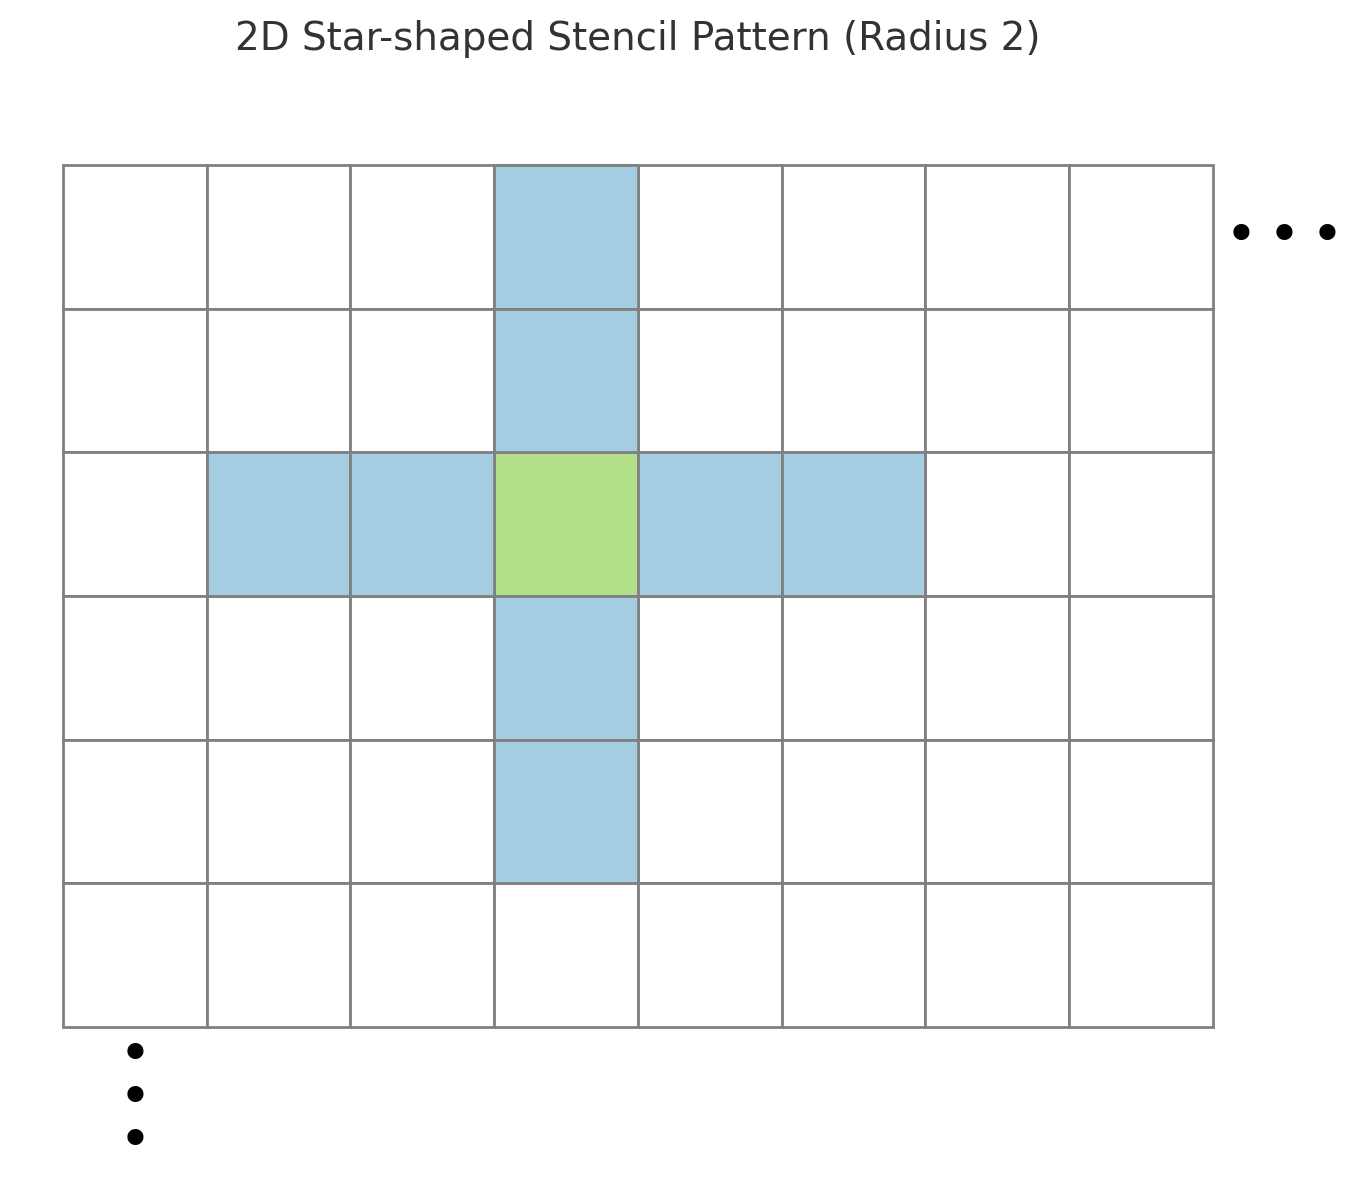
\includegraphics[width=0.5\linewidth]{stencil_visualization.png}
    \caption{A 2D star-shaped stencil pattern with radius 2}
    \label{fig:stencil_visualization}
\end{figure}

\section{The Cerebras Wafer-Scale Engine (\ac{wse})}
The Cerebras \ac{wse} has very distinct characteristics compared to both \acp{cpu} and \acp{gpu}.
Instead of memory that is separate from the compute cores, Cerebras \ac{wse} features several hundred thousand \acp{pe} that each consist of \qty{48}{\kilo\byte} of memory, a router for communication and a \ac{ce}. In contrast to traditional hardware, the memory consist solely of ultra fast \ac{sram} with a bandwidth that allows two \qty{64}{\bit} reads and one \qty{64}{\bit} write per cycle. It is laid out into eight banks with specific restrictions on which banks can be accessed at the same time.

Each fabric router has a bidirectional link to the routers of the four neighboring \acp{pe} as well as to its corresponding\ac{ce}. All of these links have a bidirectional bandwidth of \qty{32}{\bit} per cycle. So-called colors define separate virtual communication channels and can be used to configure the data flow within the \ac{wse}. Specifically, one of 24 colors can be chosen for data leaving the \ac{ce} and for each router and color a set of directions to forward incoming data to can be specified. For the \ac{wse}-2 \numproduct{66 x 154} \acp{pe} form a die and \numproduct{12 x 7} dies reside on one \qty{300}{\mm} wafer forming the \ac{wse}-2 with staggering \num{853104} physical \acp{pe}. Distinct from traditional production processes the dies are not cut, but kept together on the wafer and are linked so that the communication between \acp{pe} not only works within each die but also in between dies.
The data flow between \acp{pe} can be defined through 24 static routes called colors \cite{lie2023cerebras}.
Due to imperfect yield, some \acp{pe} are non functional.
Cerebras solves this problem by routing around these \acp{pe}. 
To make this work, the hardware includes about 1\% spare \acp{pe} so that the number of enabled \acp{pe} is a bit lower. Furthermore the \ac{wse}-2 contains \acp{pe} that are not available for the user, but are reserved for memory movement and other system functions \cite{tramm2024efficient}.
The Cerebras documentation suggests that the usable number of \acp{pe} might even slightly change from system to system \cite{cerebras_gemv_tutorial}. \citeauthor{tramm2024efficient} \cite{tramm2024efficient} find the user programmable number of \acp{pe} for \ac{wse}-2 to be \numproduct{750 x 994}, which is the number we use throughout our work. For \ac{wse}-3 the official documentation states the fabric dimensions to be \numproduct{762 x 1176} and while this does not include the spare cores, it is not clear whether the number of user-programmable \acp{pe} is the same or might be slightly lower. In the absence of official numbers, we use these throughout our work. On the \ac{wse}, each \ac{pe} has its own clock, and while these all operate at the same frequency, they are not synchronized. Although the cores are designed to run at a frequency of \qty{1.1}{\giga\hertz} \cite{lie2023cerebras}, typical deployments run at a lower frequency of \qty{850}{\mega\hertz} for \ac{wse}-2 \cite{tramm2024efficient} and \qty{875}{\mega\hertz} for \ac{wse}-3. Therefore we use these lower numbers for performance analysis throughout this work.

\begin{figure}[h]
    \centering
    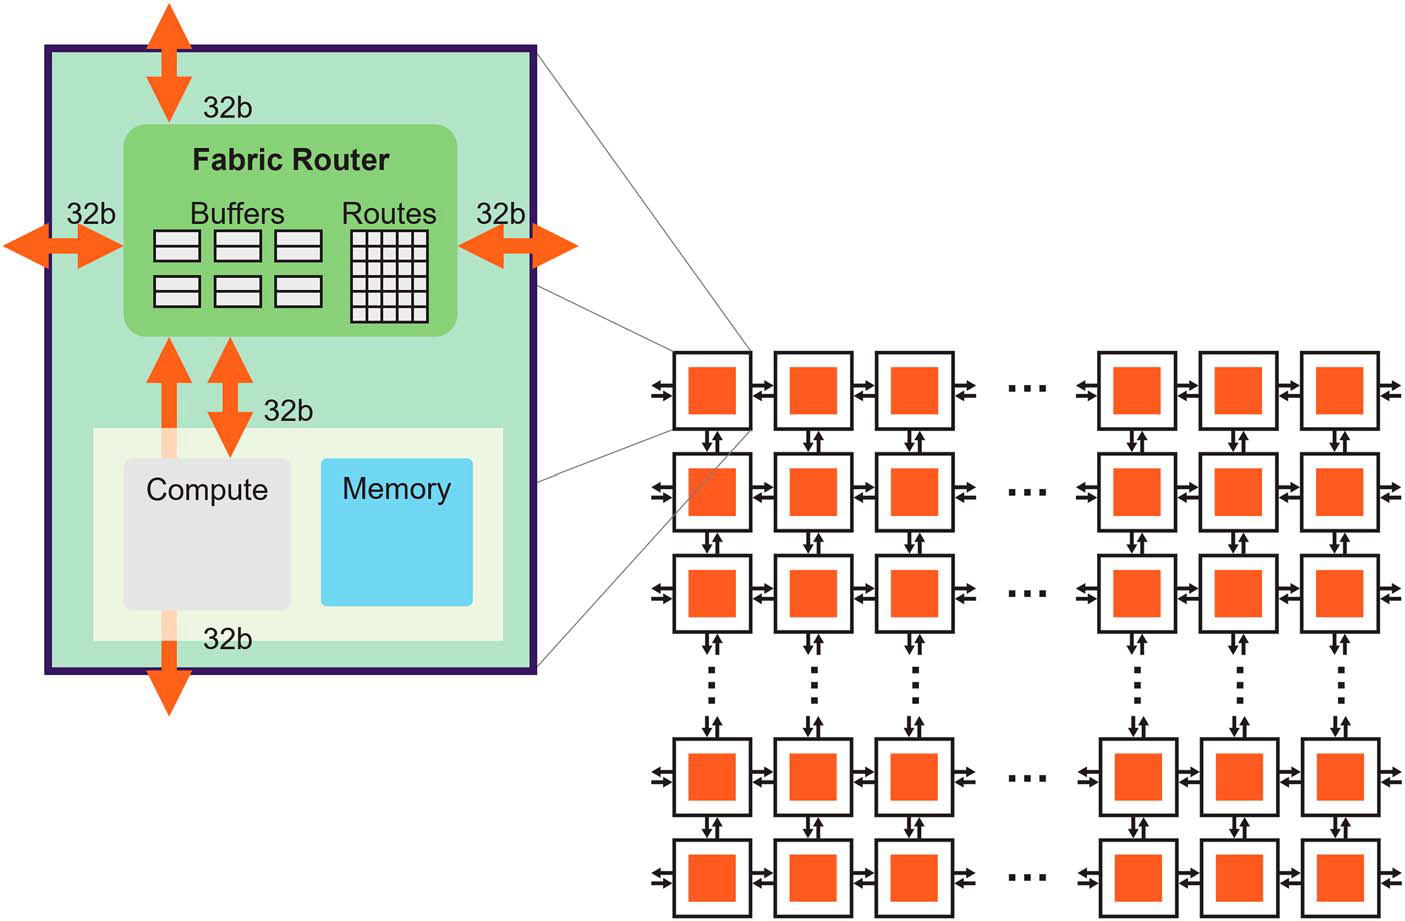
\includegraphics[width=0.5\linewidth]{wse2_pes_router.png}
    \caption{Schematic of \ac{wse}-2 processing elements arranged in a grid with interconnected routers \cite{lie2023cerebras}}
    \label{fig:wse2_pes_router}
\end{figure}

Each \ac{pe} allows to execute certain instructions in parallel with \acp{simd} units. The maximum number of parallel instructions varies between instruction types and \ac{wse} generations. Table \ref{tab:simd_operations} shows the maximum \acp{simd}-width for selected instruction types. As the \ac{wse} was originally designed for \ac{ai} workloads, the \acp{simd} units are optimized for half precision floating point operations, which are not suitable for \ac{hpc} workloads. 

\begin{table}[h]
    \centering
    \caption{Maximum \ac{simd}-width for selected instruction types}
    \label{tab:simd_operations}
    \begin{tabular}{@{}llll@{}}
        \toprule
        Op code & description & \ac{wse}-2 & \ac{wse}-3 \\
        \midrule
        \texttt{@fadds} & 32-bit floating point add & 2 & 4 \\
        \texttt{@fmuls} & 32-bit floating point multiply & 1 & 1 \\
        \texttt{@fmach} & 16-bit floating point multiply-add & 4 & 8 \\
        \texttt{@fmachs} & 16-bit floating point multiply with 32-bit addition & 2 & 4 \\
        \texttt{@fmacs} & 32-bit floating point multiply-add & 1 & 1 \\
        \texttt{@fmovs} & 32-bit floating point move & 2 & 4 \\
        \bottomrule
    \end{tabular}
\end{table}

Custom kernels for the \ac{wse} are written in \ac{csl}, a low-level language based on Zig, extended with hardware-specific features.
One of its core features is the ability to define \acp{dsd} which define data access patterns including a base memory address, an offset, a stride and a length. They can be used for up to four dimensional tensors. Specifically, there are four \ac{dsd} types: \texttt{mem1d\_dsd}, \texttt{mem4d\_dsd}, \texttt{fabin\_dsd} and \texttt{fabout\_dsd}. While \texttt{fabin\_dsd} and \texttt{fabout\_dsd} are used for fabric communication and \texttt{mem1d\_dsd} are used for one dimensional arrays, \texttt{mem4d\_dsd} are somewhat unintuitively used for tensors with two, three, or four dimensions. The \ac{wse}-2 has 44 \acp{dsr} per \ac{pe}, which are hardware registers used to hold \acp{dsd}. These can be used directly as operands for instructions. Loading \acp{dsd} into \acp{dsr} is done automatically by the compiler, but can also be done manually and enables the programmer to optimize the code. Communication between \acp{pe} is handled with special fabin- and fabout-\acp{dsd}, describing data that is sent to or received from a neighboring \ac{pe}.

The routers contain a limited number of input and output queues, small physical buffers for incoming and outgoing data.

\ac{csl} has limited support for concurrency which is enabled by the use of tasks that are activated by events like completion of an asynchronous communication or computation. Due to the single thread of execution, there is no true parallelism within a single \ac{pe}.

\chapter{Related Work}
The inherently low arithmetic intensity of stencil codes made their optimization a long-standing research topic.
Most work for traditional \ac{hpc} architectures like \ac{cpu} and \ac{gpu} focuses on cache optimization by using techniques like tiling, loop transformations or temporal blocking, that increases the effective arithmetic intensity and shift the problem more towards being compute-bound.
Tiling improves the cache utilization by splitting the problem domain spatially into parts, so that cached values can be used for as many updates as possible.
Tiling can be implemented hierarchically for all cache levels.
Temporal blocking takes the concept of tiling a step further by performing multiple iterations on a single tile before moving to the next tile.
Bringing all of these techniques together for a specific application is inherently complex and requires careful tuning, taking into accounst the specific hardware cache sizes, the problem size and stencil layout.
This raised the need for specialized stencil compilers.
One of these is Devito, a python based \ac{dsl} for finite difference stencil codes, that generates code for different \ac{hpc} architectures, incorporating various optimization techniques \cite{lange2016devito}. 
Other systems include Tiramisu, ExaStencils and Pochoir which uses a divide-and-conquer algorithm to make it oblivious to the cache size \cite{baghdadi2019tiramisu,lengauer2014exastencils,tang2011pochoir}.

However, new hardware accelerators like the \ac{wse} feature a vastly different programming model with \acp{pe} representing independent hardware units with a lack of synchronized control, distributed memory and a completly missing cache hierarchy. 
This makes most studied ideas not applicable and left the limiting factors of stencil codes on the \ac{wse} underexplored and too difficult to target for general-purpose stencil compilers.

\citeauthor{rocki2020fast} \cite{rocki2020fast} were the first to use the \ac{wse} architecture for stencil computations and showcased an efficient 7-point 3D stencil for finite differences.
They laid the foundation for how the memory access in stencil patterns can be replaced by communication between \ac{pe}s holding parts of the grid. They do this by mapping the z-dimension of the grid to the \ac{pe}s memory while mapping the x and y dimensions to the \ac{wse}-2's \ac{pe}s, so that each \ac{pe} holds a 1D column of the grid.
Building on this work, \citeauthor{jacquelin2022scalable} \cite{jacquelin2022scalable} implement and analyze a more complex 25-point 3D stencil on the \ac{wse}-2. Different than the work done by \citeauthor{rocki2020fast} \cite{rocki2020fast}, this stencil requires multi-hop communication, which involves complex dynamic routing configurations.
Noticably they show almost perfect weak scaling with an increasing number of \ac{pe}s, meaning that when the number of \ac{pe}s is increased from \numproduct{200 x 200} to the full \ac{wse}-2's maximum dimension of \numproduct{755 x 994} while increasing the problem size by the same factor, the runtime is almost constant with only a 1.5\% increase.

There have also been apporaches working on abstracting away as much complexity as possible and automatically generate \ac{csl} from a higher level \ac{api} or stencil \ac{dsl} as presented by \citeauthor{woo2022disruptive} \cite{woo2022disruptive} and \citeauthor{sai2024automated} \cite{sai2024automated}. However, these approaches focus on 3D stencils and while they might be able to generate code for 2D stencils, they don't explore topics like tiling of the x and y dimensions. While this idea is less practical for most 3D stencil applications, it is a lot more promising for 2D stencils and therefore the focus of our work. We furthermore systematically analyze the performance implications of different tile sizes and radii, directly comparing low-order and high-order stencil patterns on the \ac{wse}.
\chapter{Implementation}
Since communication on Cerebras hardware is limited to the four direct neighbor elements, stencil algorithms that for a single iteration require data from \acp{pe} that are not direct neighbors are far more complex to implement and come with significant communication overhead. For that reason, we limit the scope of this work to update functions that require only communication with the direct neighboring \acp{pe}. This means that the radius of the stencil must be small or equal to the tile size, specifically
\begin{equation}    
\label{eq:radius_constraint}
r \leq \min(t_w, t_h)
\end{equation}

For the simple case where $t_w=t_h=1$, this results in a radius of 1.

Two approaches were implemented:
\begin{itemize}
    \item In specialized version, that restricts the radius to one represents each element of the grid with one \ac{pe} of the \ac{wse}. This specialization allows a heavily optimized implementation, but restricts the maximum problem size to the \ac{wse} hardware dimensions.
    \item A general implementation maps multiple elements of the underlying grid, i.e., a tile size of $t_w, t_h$, to a single \ac{pe} and therefore allows for grid sizes that significantly exceed the \ac{wse} hardware dimensions and a radius greater than one as long as \autoref{eq:radius_constraint} is satisfied. 
\end{itemize}

\section{radius-1, non-tiled}
The computation for each element can be described as follows:
\begin{equation}
    \label{eq:stencil_computation}
    v^{'} = w_0 \cdot v + w_1 \cdot (v_{north} + v_{east} + v_{south} + v_{west})
\end{equation}
Where $v$ is the old value of the element, $v_{north}, v_{east}, v_{south}, v_{west}$ are the values of the four neighbors, $w_0, w_1$ are the stencil coefficients and $v^'$ is the new value of the element.

\subsection{Routing configuration}
Each \ac{pe} must be able to send its data to, and receive data from its four direct neighboring \acp{pe}. Notably it sends the same data to the four neighbors. This allows for increasing communication speed by sending the data only once and forwarding it in the router to all neighbors. We used a pattern containing six distinct colors to map the grid.
The coloring rule can be described as following function $f:\mathbb{N}\times\mathbb{N}\to\{0,1,2,3,4,5\}$:
\begin{equation}
    \label{eq:coloring_function}
    f(x,y) = (x + 2y) \bmod 6
\end{equation}
and visualized in \autoref{fig:r1_stencil_coloring}.
\begin{figure}
    \centering
    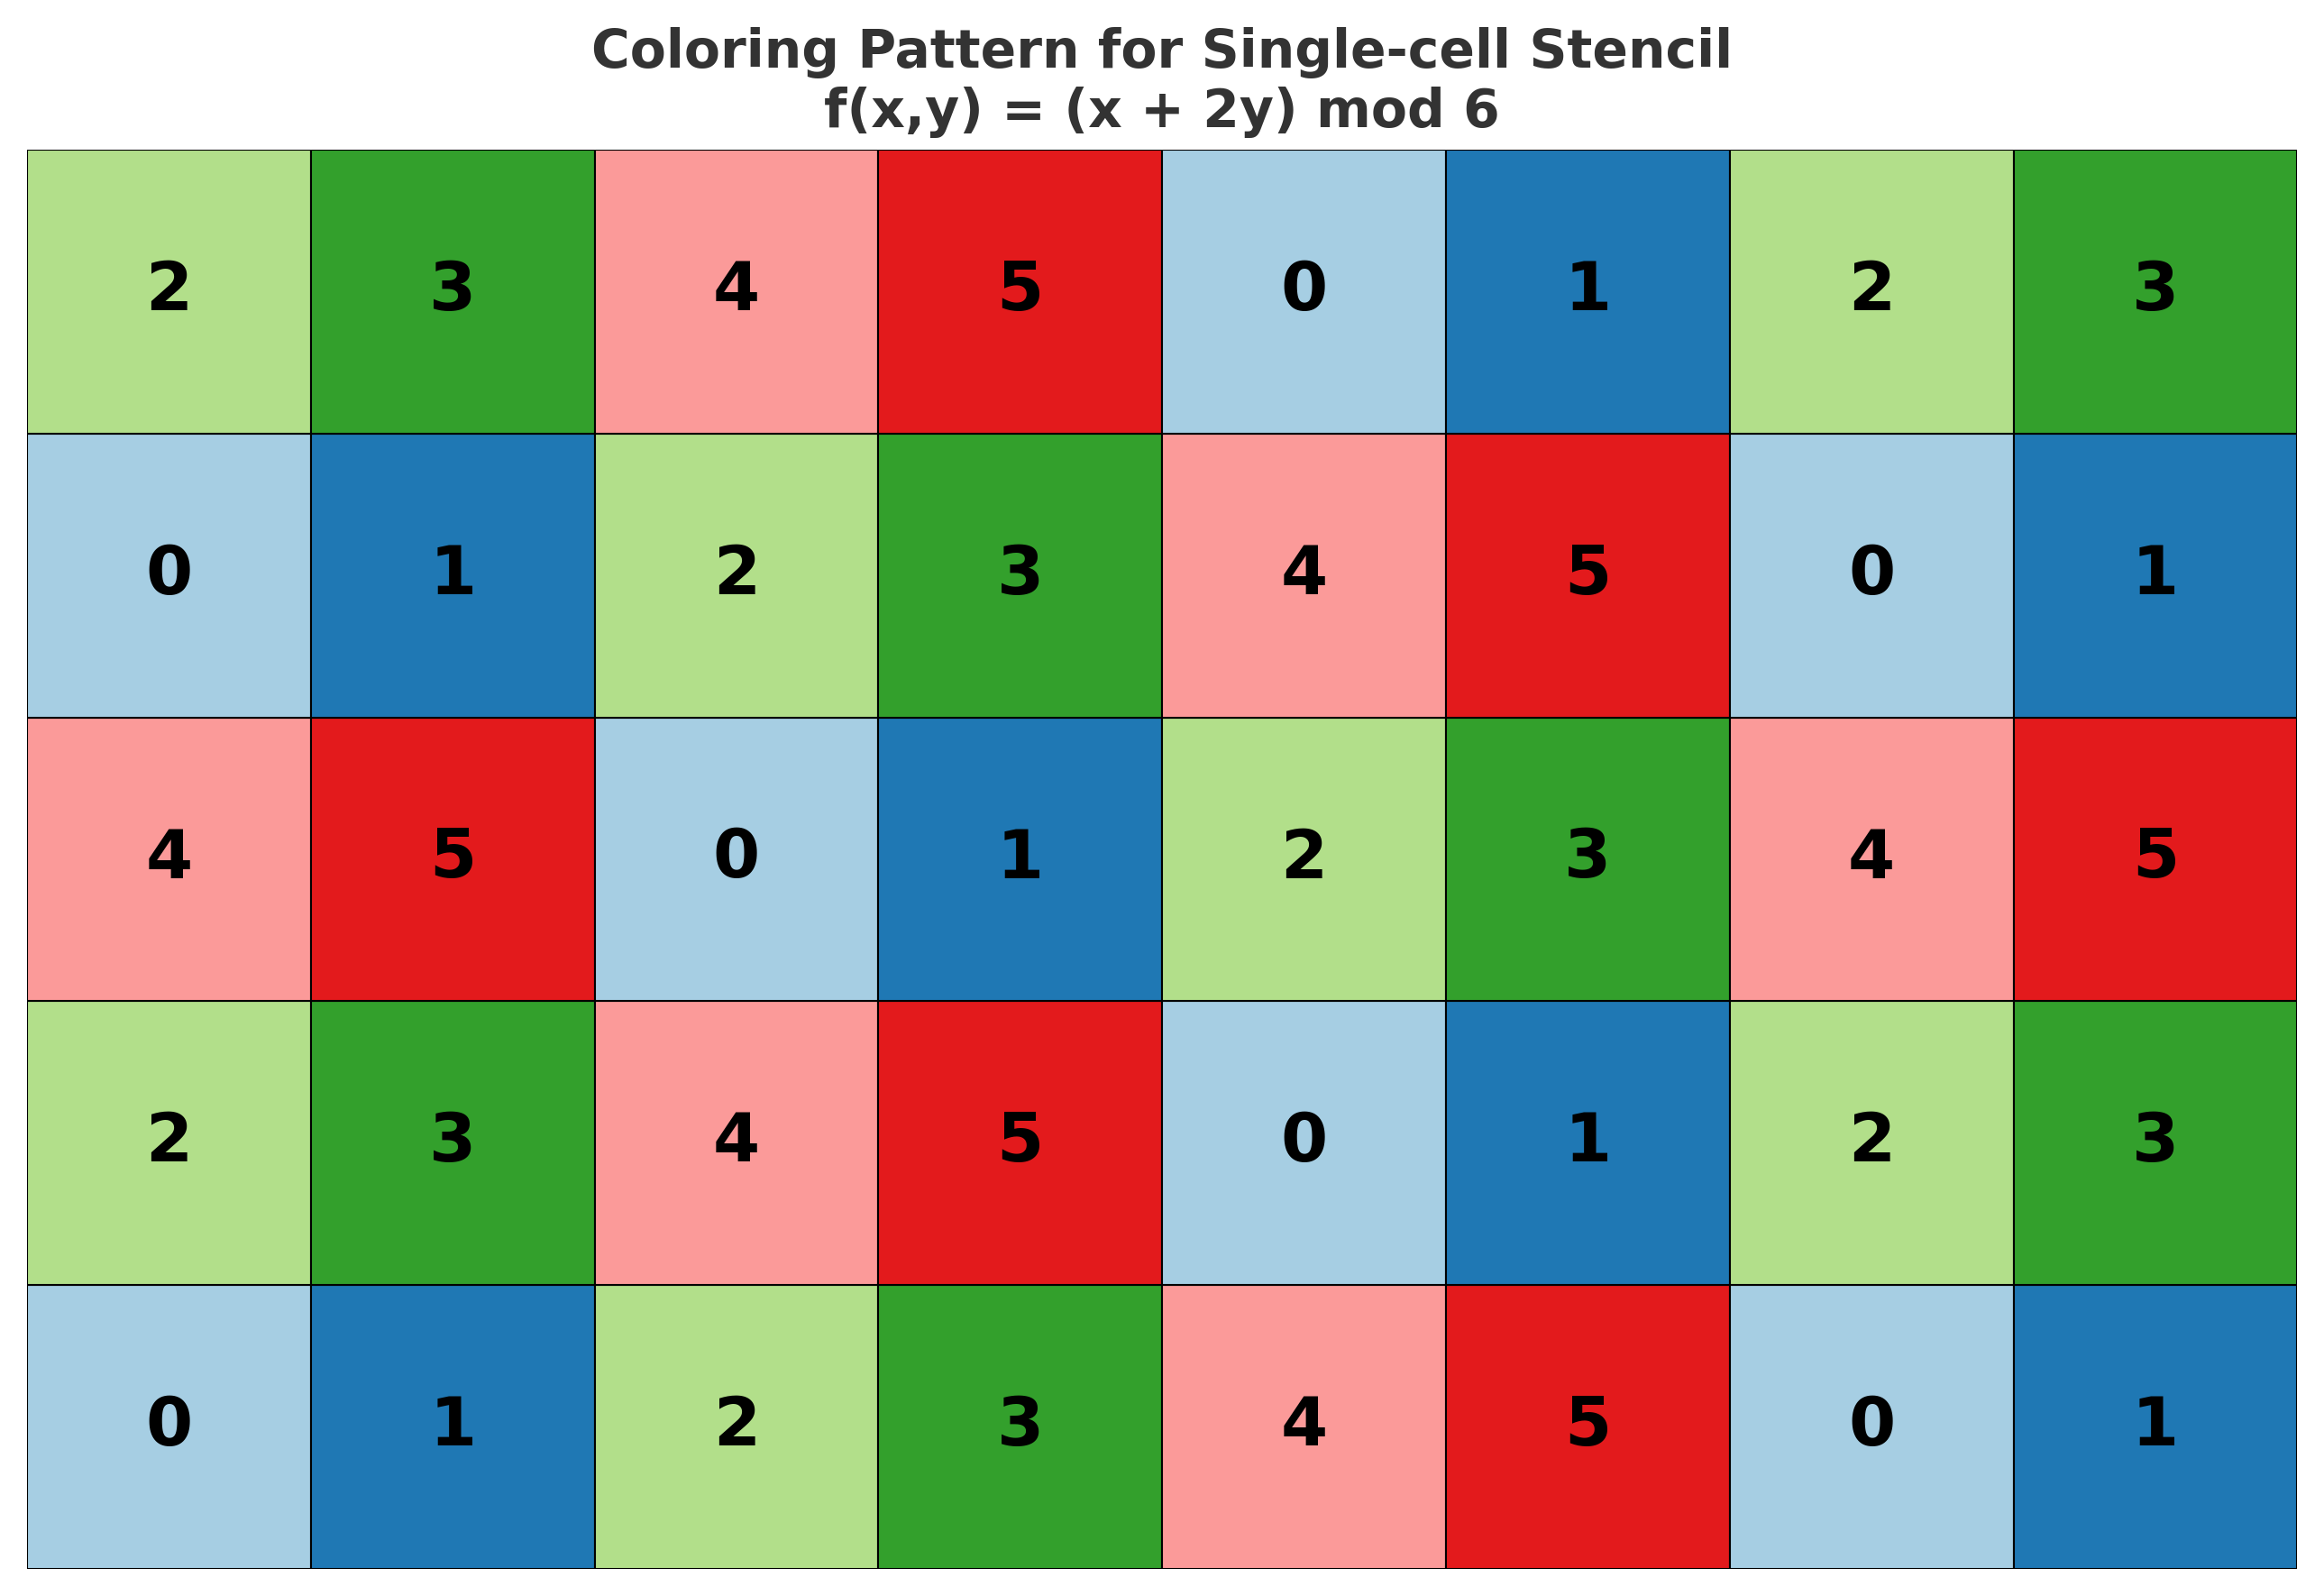
\includegraphics[width=0.5\linewidth]{r1-stencil-coloring.png}
    \caption{Visualization of the coloring pattern for radius-1 non-tiled stencil. Each color represents a distinct routing color (0-5) used for conflict-free communication between \acp{pe}. The numbers in each cell show the color index computed by $f(x,y) = (x + 2y) \bmod 6$.}
    \label{fig:r1_stencil_coloring}
\end{figure}

\subsection{\ac{pe} Program}
The implementation for the radius-1, non-tiled case is relatively simple.
Although only single elements are processed at a time, \acp{dsd} are needed for communication and for performance reasons explicit \ac{dsr} assignment is employed, decreasing the number of cycles per iteration significantly.  
Further, the center multiplication is placed at the beginning of each iteration in a way that it overlaps with the communication delay and does not need an additional cycle.
Because only one fp32 element is received from and send to each neighbour, input- and output- queues never fill up completely and synchronous \ac{dsd} operations can be used instead of asynchronous operations that add significant overhead.
Furthermore, the algorithm multiplies the value which is send to the neighbors with the coefficient $w_1$ while sending, so that the receiving \acp{pe} only add these values to $w_0 \cdot v$ to get the new value.
By computing the intermediate values $intermediate_1$ and $intermediate_2$ before adding them to $value$, the number of cycles for this part of the calculation is reduced from 10 to 7.

\begin{algorithm}[tbh]
    \SetAlgoLined
    \KwData{Received values from neighbors}
    \KwResult{Updated value}
    $intermediate_1 \gets \Call{ReceiveFromNorth}{} + \Call{ReceiveFromEast}{}$\;
    $intermediate_2 \gets \Call{ReceiveFromSouth}{} + \Call{ReceiveFromWest}{}$\;
    $value \gets value + intermediate_1$\;
    $value \gets value + intermediate_2$\;
    \caption{Algorithm with intermediate values}\label{alg:intermediate_values}
\end{algorithm}

While the reason for this performance benefit cannot be explained by the publicly available documentation from Cerebras, speculation from limited testing suggests that values seem to be available to a following operation only three cycles after they were written to.
Our empirical analysis revealed a data dependency stall: an operation using a register as an operand is delayed until at least three cycles have passed since that register was last written to. While this behavior is not detailed in the public documentation, it consistently impacts performance. By reordering the computation to use intermediate variables (as shown in \autoref{alg:intermediate_values}), we mitigate these stalls, reducing the cycle count for this computational segment from 10 to 7 cycles.

Unfortunately, this does not work on WSE-3, since it allows at most one fabric \ac{dsd} arguments per operation.

\begin{table}[h]
    \centering
    \caption{Operations for one grid point and iteration in the radius-1, non-tiled implementation.}
    \label{tab:r1_non_tiled_operations}
    \begin{tabular}{@{}cccc@{}}
        \toprule
        Operation & Cerebras Op Code & Count & Flops \\
        \midrule
        add & \texttt{@fadds} & \num{4} & \num{4} \\
        mul & \texttt{@fmuls} & \num{2} & \num{2} \\
        \midrule
        total & & \num{6} & \num{6} \\
        \bottomrule
    \end{tabular}
\end{table}

\section{tiled any radius star shaped 2d}
For a radius greater than one, the computation can be expressed as follows:
\begin{equation}
    \label{eq:stencil_computation_tiled}
    v^{'} = w_0 \cdot v + \sum_{i=1}^{r} w_i \cdot (v_{north,i} + v_{east,i} + v_{south,i} + v_{west,i})
\end{equation}
Where $v$ is the old value of the element, $v_{north,i}, v_{east,i}, v_{south,i}, v_{west,i}$ are the values of the four neighbors at distance $i$ from the center and $w_0, w_1, \dots, w_r$ are the stencil coefficients.

\subsection{Routing configuration}
\begin{figure}
    \centering
    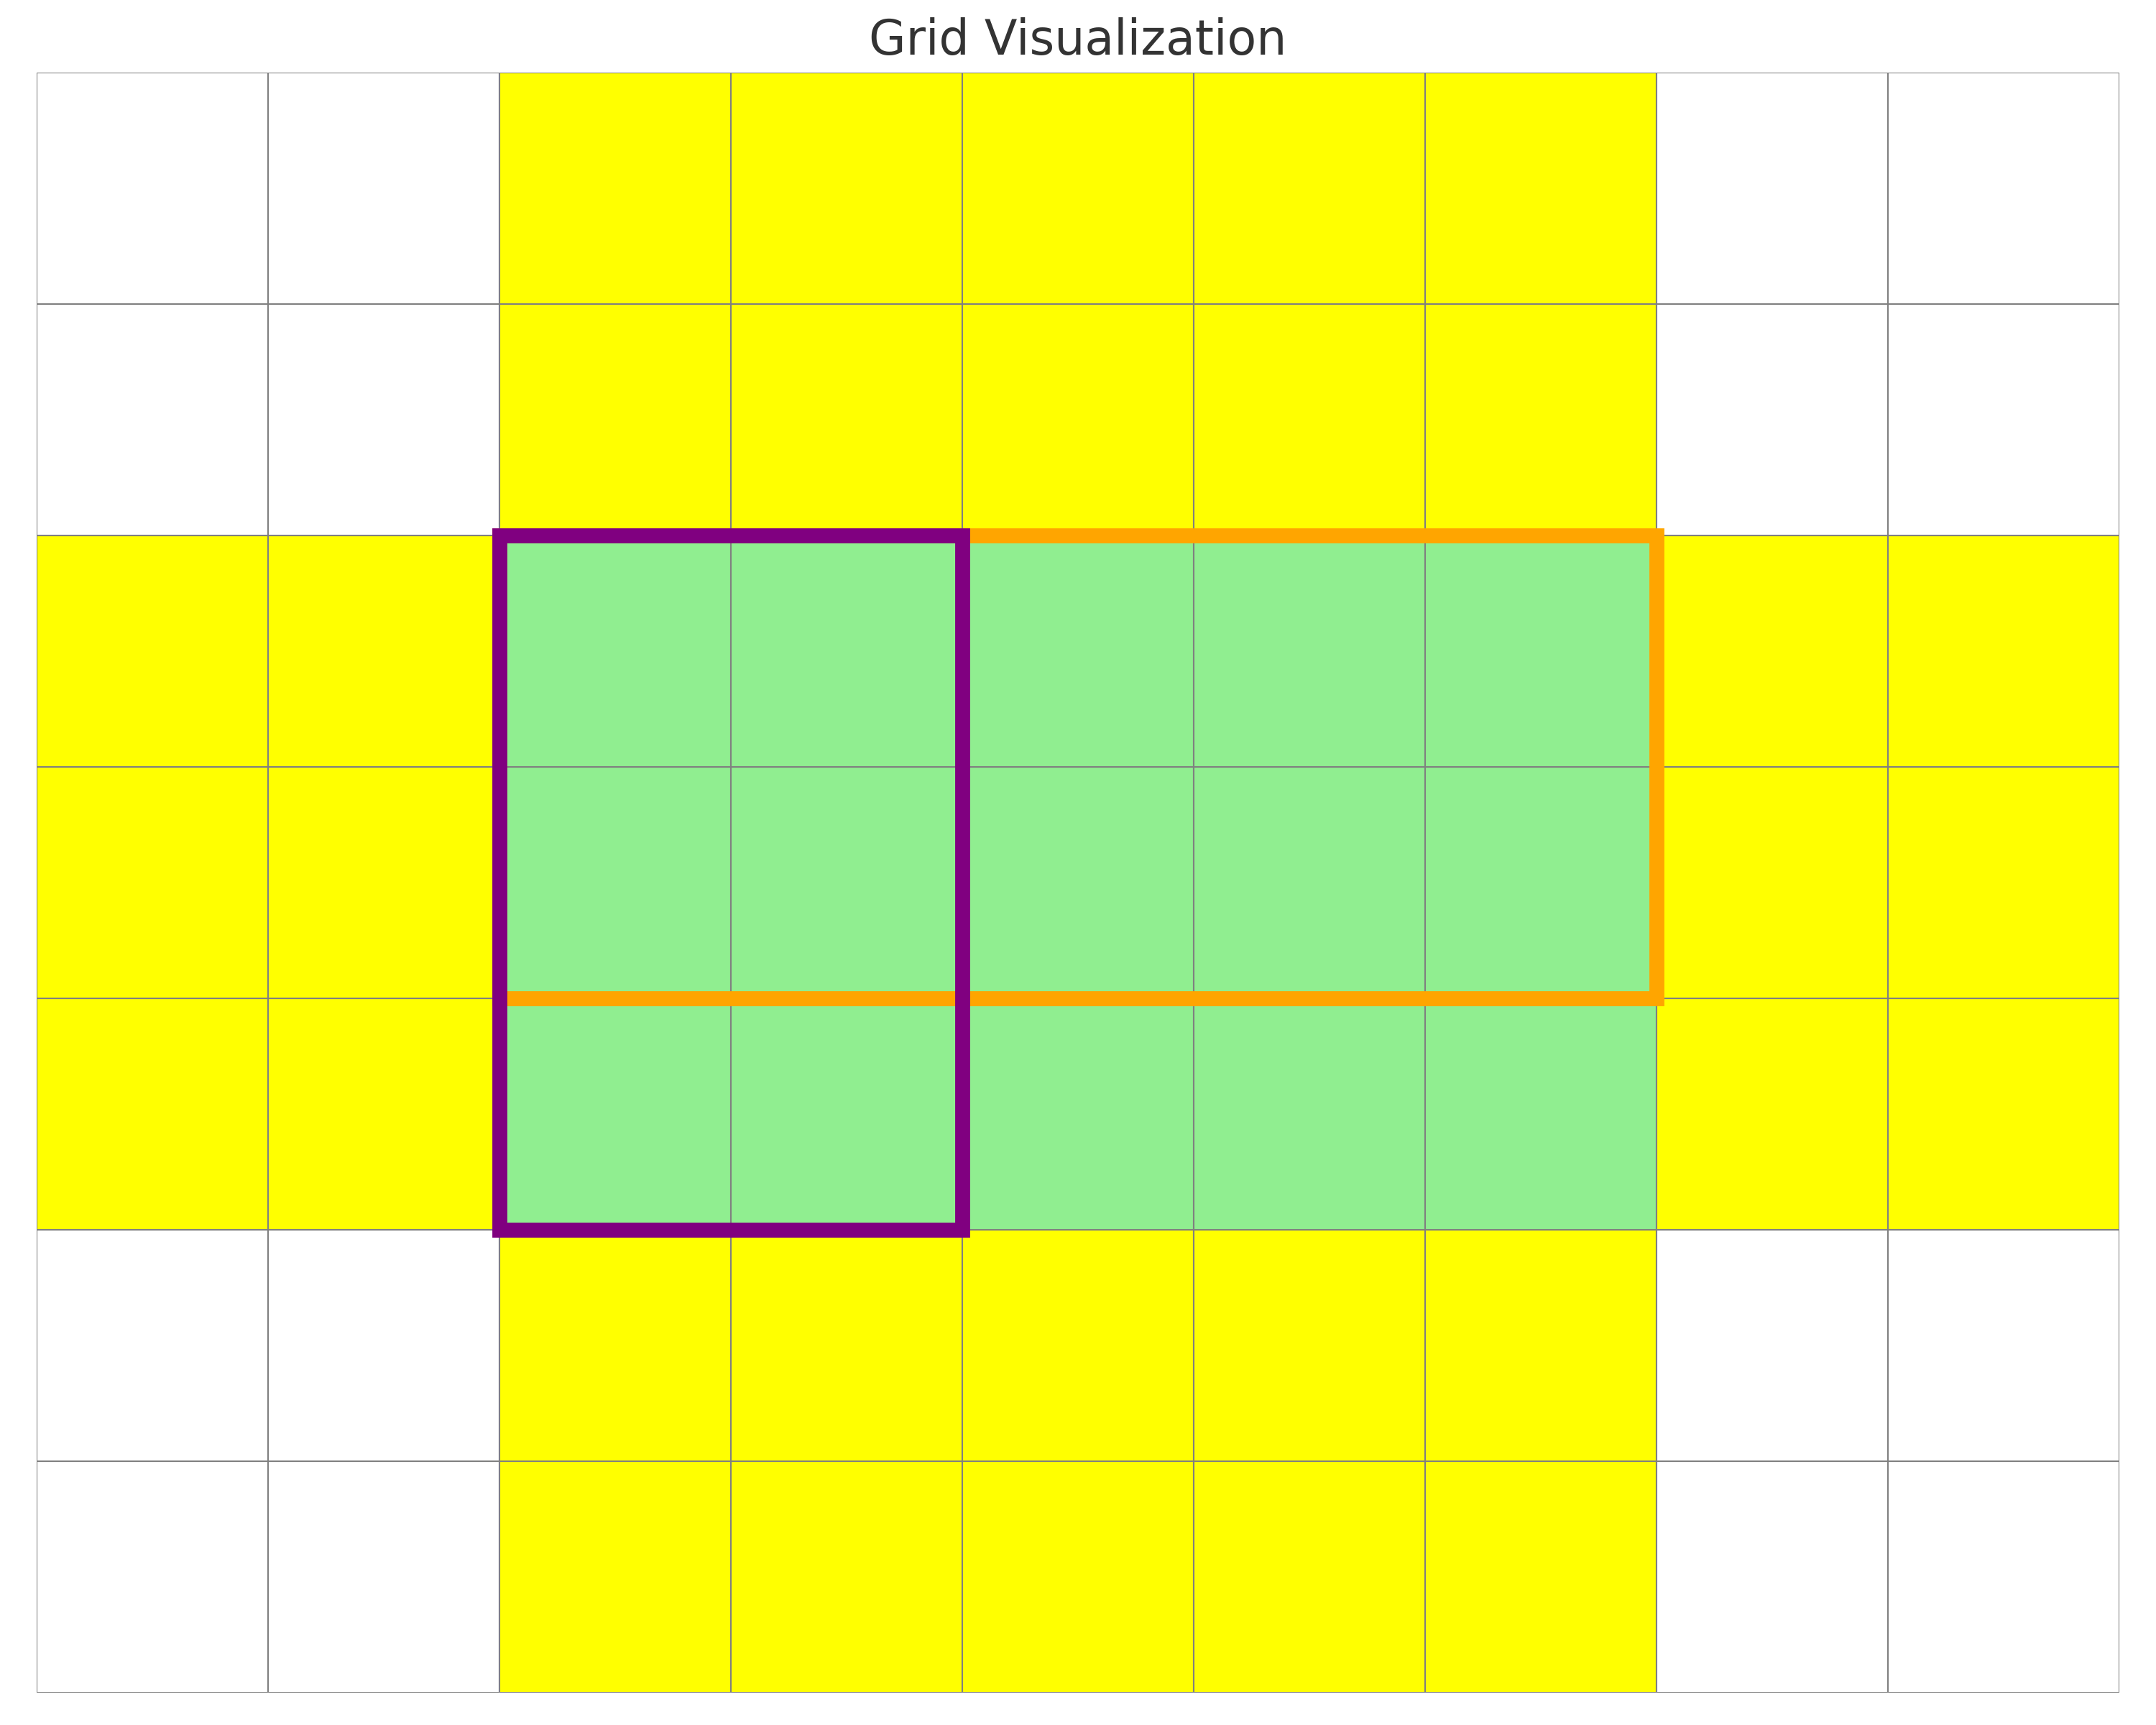
\includegraphics[width=0.5\linewidth]{grid_visualization.png}
    \caption{Data layout within a single PE for a tiled stencil with tile size $t_w=5, t_h=3$ and radius $r=2$. The green area represents the PE's assigned grid tile. The surrounding yellow halo region stores data received from neighbors, while the orange and purple outlines show the data regions sent to the northern and western PEs, respectively.}
    \label{fig:grid_visualization}
\end{figure}
The communication for the variable tile size requires one \ac{pe} to send different data to its neighbors. This is visualized in \autoref{fig:grid_visualization}. This requires four distinct colors for sending to the different neighbors as well as four colors to receive. For each of the four directions, a pair of colors is used and arranged in a checkerboard pattern across the \ac{pe}-grid.
If colors 0 and 1 are used for data transfer from west to east, following function can be used to determine what color is used to send and to receive:
\begin{equation}
    \label{eq:tiled_coloring_function}
    f(row, col)=(row+col) \bmod 2
\end{equation}
Where $f$ determines the color used to send data east and $1-f$ is used to receive from west. The same method is also applied for the other directions.

\subsection{\ac{pe} Program}

\begin{figure}
    \centering
    \animategraphics[autoplay,loop,controls=false,width=\linewidth]{0.5}{stencil_frames/frame_0}{0}{8}
    \caption{Animation of the computational steps for one iteration of the tiled algorithm with radius $r=2$. Each frame highlights the rectangular region of the buffer being accessed and multiplied by a weight, with the result accumulated. The sequence demonstrates how the algorithm iterates through the halo regions as the values for the next iteration are computed. (Note: Animation may require a compatible PDF viewer).}
    \label{fig:stencil_algorithm_animation}
\end{figure}

The tile of the grid, held by single \ac{pe} is stored in the center region of a 2D array of size $(t_h+2r)\times (t_w+2r)$ - the $buffer$. This array is larger than the tile itself to allow for the halo region, which is used to store the data received from the neighbors. Furthermore an accumulator array of the same size is used to store the intermediate values of the stencil computation. In this array, only the center of size $t_h, t_w$ is used. Choosing its size to be the same as the buffer leads to more consistent memory access patterns, which reduces bank conflicts.

Two \texttt{mem4d\_dsd}s per direction are used for communication. One that specifies the location within the buffer of the data to send and one that specifies the location of the data to receive.
Asynchronous \texttt{@fmovs} instructions are used for data exchange. Two counters track the completion of asynchronous send and receive operations. Once all four neighbor data blocks have been sent and all four have been received, the main computation task is triggered. This ensures that the computation only starts once all necessary data is available in the halo regions.

A \ac{dsd} is used to select the center region of the buffer. This \ac{dsd} is subsequently shifted to represent a rectangular area of the buffer that is shifted up, down, left or right by a number of elements up to the radius from the center. \texttt{@fmacs} instructions are used to multiply these values with the respective weight and add the results to the accumulator. The accumulator is then multiplied with the weight $w_0$ and added to the center region of the buffer to complete the iteration. This process is visualized in \autoref{fig:stencil_algorithm_animation}.

If only \texttt{@fmacs} instructions were used, the accumulator would have to be reset to zero after each iteration. To avoid this, a \texttt{@fmuls} instruction is used for the very first operation that writes to the accumulator to overwrite the values of the previous iteration.

\begin{algorithm}[tbh]
    \SetAlgoLined
    \KwData{Buffer with halo regions filled}
    \KwResult{Updated buffer center}
    \For{$i \gets 1$ \KwTo $r$}{
        \eIf{$i == 1$}{
            $accumulator \gets weights[i] \cdot buffer\_center\_dsd_{UP,i}$\;
        }{
            $accumulator \gets accumulator + weights[i] \cdot buffer\_center\_dsd_{UP,i}$\;
        }
        $accumulator \gets accumulator + weights[i] \cdot buffer\_center\_dsd_{DOWN,i}$\;
        $accumulator \gets accumulator + weights[i] \cdot buffer\_center\_dsd_{LEFT,i}$\;
        $accumulator \gets accumulator + weights[i] \cdot buffer\_center\_dsd_{RIGHT,i}$\;
    }
    $buffer\_center\_dsd \gets buffer\_center\_dsd + weights[0] \cdot accumulator$\;
    \caption{Tiled algorithm code}\label{alg:tiled_algorithm}
\end{algorithm}

The dicrilet border is implemented by using a ring of \acp{pe} that only send and receive data from their neighbors and do not participate in the computation. If $r<t_w$ or $r<t_h$ the border \acp{pe} values are padded with zeros to fill their buffer. Re refer to the \acp{pe} that only send and receive data from their neighbors as border \acp{pe}, the ones that participate in the computation as inner \acp{pe} and the set of both of these as active \acp{pe}.

\begin{table}[h]
    \centering
    \caption{Operations for one grid point and iteration, tiled implementation with radius $r$.}
    \label{tab:tiled_operations}
    \begin{tabular}{@{}cccc@{}}
        \toprule
        Operation & Cerebras Op Code & Count & Flops \\
        \midrule
        fmac & \texttt{@fmacs} & $5r-1$ & $10r-2$ \\
        mul & \texttt{@fmuls} & \num{1} & \num{1} \\
        \midrule
        total & & $5r$ & $10r-1$ \\
        \bottomrule
    \end{tabular}
\end{table}

As a special case of the tiled algorithm, the radius-1 problem was further optimized by using \texttt{mem1d\_dsd}s instead of \texttt{mem4d\_dsd}s for the halo regions where the neighbors data is received as well as the data to send. Furthermore the shifted \acp{dsd} are precomputed and all \acp{dsd} are explicitly assigned to distinct \acp{dsr}. There are enough \acp{dsr} available so that each \ac{dsr} is used for at most one \ac{dsd}. This allows for a significant reduction in the number of cycles per iteration, since loading the \acp{dsd} into \acp{dsr} only needs to be done once, independent of the number of iterations. We still find that the \acp{dsd} used for reading the parts of the buffer that are send to the neighbors and the ones describing the halo regions for receiving need to be reloaded to the \acp{dsr} for each iteration. The load to \ac{dsr} for these \acp{dsd} acts as a kind of reset and if not done, it leads to buffer overflows. The documentation doesn't specify this requirement and interestingly, it is not necessary for all \acp{dsd}. 
As another optimization, \texttt{@fadds} are used instead of \texttt{@fmacs} and the multiplication is handled separately. This reduces the flop number from $9$ to $6$ per element and results in a performance improvement because the simd width for \texttt{@fadds} is 2/4 on wse-2/3 while it is only 1 for \texttt{@fmacs}. Note that the shifted \acp{dsd} $buffer\_center\_dsd_{DIR,i}$ in the general version need to be created for each iteration of the loop while pre-computed \acp{dsd} are used in this optimized version.

We refer to this as the r1 optimized version of the tiled algorithm.
The tiled algorithm is implemented so that it automatically selects the r1 optimized version if the radius is 1.
For all experiments in this work, the r1 optimized version is used whenever applicable, except when explicitly stated otherwise.

\begin{algorithm}[tbh]
    \SetAlgoLined
    \KwData{Buffer with halo regions filled}
    \KwResult{Updated buffer center}
    $accumulator \gets buffer\_center\_dsd \cdot weights[0]/weights[1]$\;
    $accumulator \gets accumulator + buffer\_center\_dsd_{UP,1}$\;
    $accumulator \gets accumulator + buffer\_center\_dsd_{DOWN,1}$\;
    $accumulator \gets accumulator + buffer\_center\_dsd_{LEFT,1}$\;
    $accumulator \gets accumulator + buffer\_center\_dsd_{RIGHT,1}$\;
    $buffer\_center\_dsd \gets buffer\_center\_dsd + accumulator \cdot weights[1]$\;
    \caption{Radius-1, tiled algorithm code}\label{alg:r1_tiled_algorithm}
\end{algorithm}

\begin{table}[h]
    \centering
    \caption{Operations for one grid point and iteration, r1 optimized tiled implementation.}
    \label{tab:tiled_operations_r1_optimized}
    \begin{tabular}{@{}cccc@{}}
        \toprule
        Operation & Cerebras Op Code & Count & Flops \\
        \midrule
        add & \texttt{@fadds} & \num{4} & \num{4} \\
        mul & \texttt{@fmuls} & \num{2} & \num{2} \\
        \midrule
        total & & \num{6} & \num{6} \\
        \bottomrule
    \end{tabular}
\end{table}

With a larger tile size, the explicit starting mechanism of the computation task can be skipped so that the computation task can be activated while the data is send and received. Explicitly specified task priorities lead to the computation task only being executed after all data is send and received. However, this only works for WSE-3. 
\chapter{Theoretical Performance Evaluation and Comparison against Roofline Model}
\label{sec:theory_performance}
actual roofline plot 

In this section the theoretical best performance of the implemented algorithms given the Cerebras hardware constraints is analyzed.
We assume the data type to be float32.
The cycle count for one iteration of the stencil is limited by following factors:
\begin{itemize}
    \item Communication time, i.e. total amount of data send and received per iteration divided by link throughput
    \item Computation time, i.e. total amount of computation per iteration divided by computation throughput
    \item Communication delay, i.e. total amount of time spent waiting for data while no computation can be done
\end{itemize}

\section{Radius 1, no tiling}
The \ac{ce} must receive the values from its four neighbors. Since the link capacity between the router and \ac{ce} is 32 bit per cycle, this will take four cycles in the best case.

The received data can immediately be used for computation as the \texttt{@fadds} and \texttt{@fmacs} commands can use dsds of type \texttt{fabin\_dsd} as an input. This means most of the computation can be done during the receiving of the data. Only one extra cycle is necessary to take into account the old $value$. With a clever implementation this extra computation could be executed during the communication delay idle time so that it doesn't affect the overall cycle count.

Sending takes one cycle from \ac{ce} to its router, another cycle from the router to its neighbors routers and a third cycle from these routers to the neighbors \acp{ce}. This results in three cycles for the communication delay.

In total this results in seven cycles per stencil operation that could be archived in theory.
Note that this is independent of the actual grid size (as long as it fits onto the \ac{wse}).

\section{Any radius and tiling}
Similarly to before the total computation for one iteration can be split up into the same three fundamental steps. We now need to take the radius $r$, tile width $t_w$ and tile height $t_h$ into account.

Each \ac{pe} needs data from its four neighbors. $r\cdot t_w$ elements from the northern and southern neighbors and $r\cdot t_h$ elements from the western and eastern neighbors. This results in $2r(t_w+t_h)$ total elements and cycles for data receiving.

During the computation $4r+1$ multiply-add operations per grid element are required which results in $t_wt_h(4r+1)$ multiply-add operations per \ac{pe}. With SIMD execution we can parallelize this and divide it by the SIMD width for \texttt{@famcs} which is 4 on wse-2 and 8 on wse-3. This results in $\left\lceil\frac{t_wt_h(4r+1)}{s}\right\rceil$. This term exceeds the communication term for most parameter combinations of $t_w,\ t_h$ and $r$. Assuming the first part of the computation could still be done during communication, we can drop the communication term completely. Note that this is a rather optimistic assumption and likely not achievable with the hardware.

The communication delay is in this case negligible and could be overlapped with the computation in a way that it doesn't affect the cycle count. 

This results in a total cycle count of $\left\lceil\frac{t_wt_h(4r+1)}{s}\right\rceil$ which is just the computation time and assuming we can fully overlap the communication time as an optimistic estimate. As a slightly pessimistic estimate we get $\left\lceil\frac{t_wt_h(4r+1)}{s}\right\rceil+2r(t_w+t_h)$ which assumes no possible overlap between communication and computation. 

It becomes clear that for radius 1 the tiled stencil gets significantly slower than the non-tiled implementation. 
\begin{figure}
    \centering
    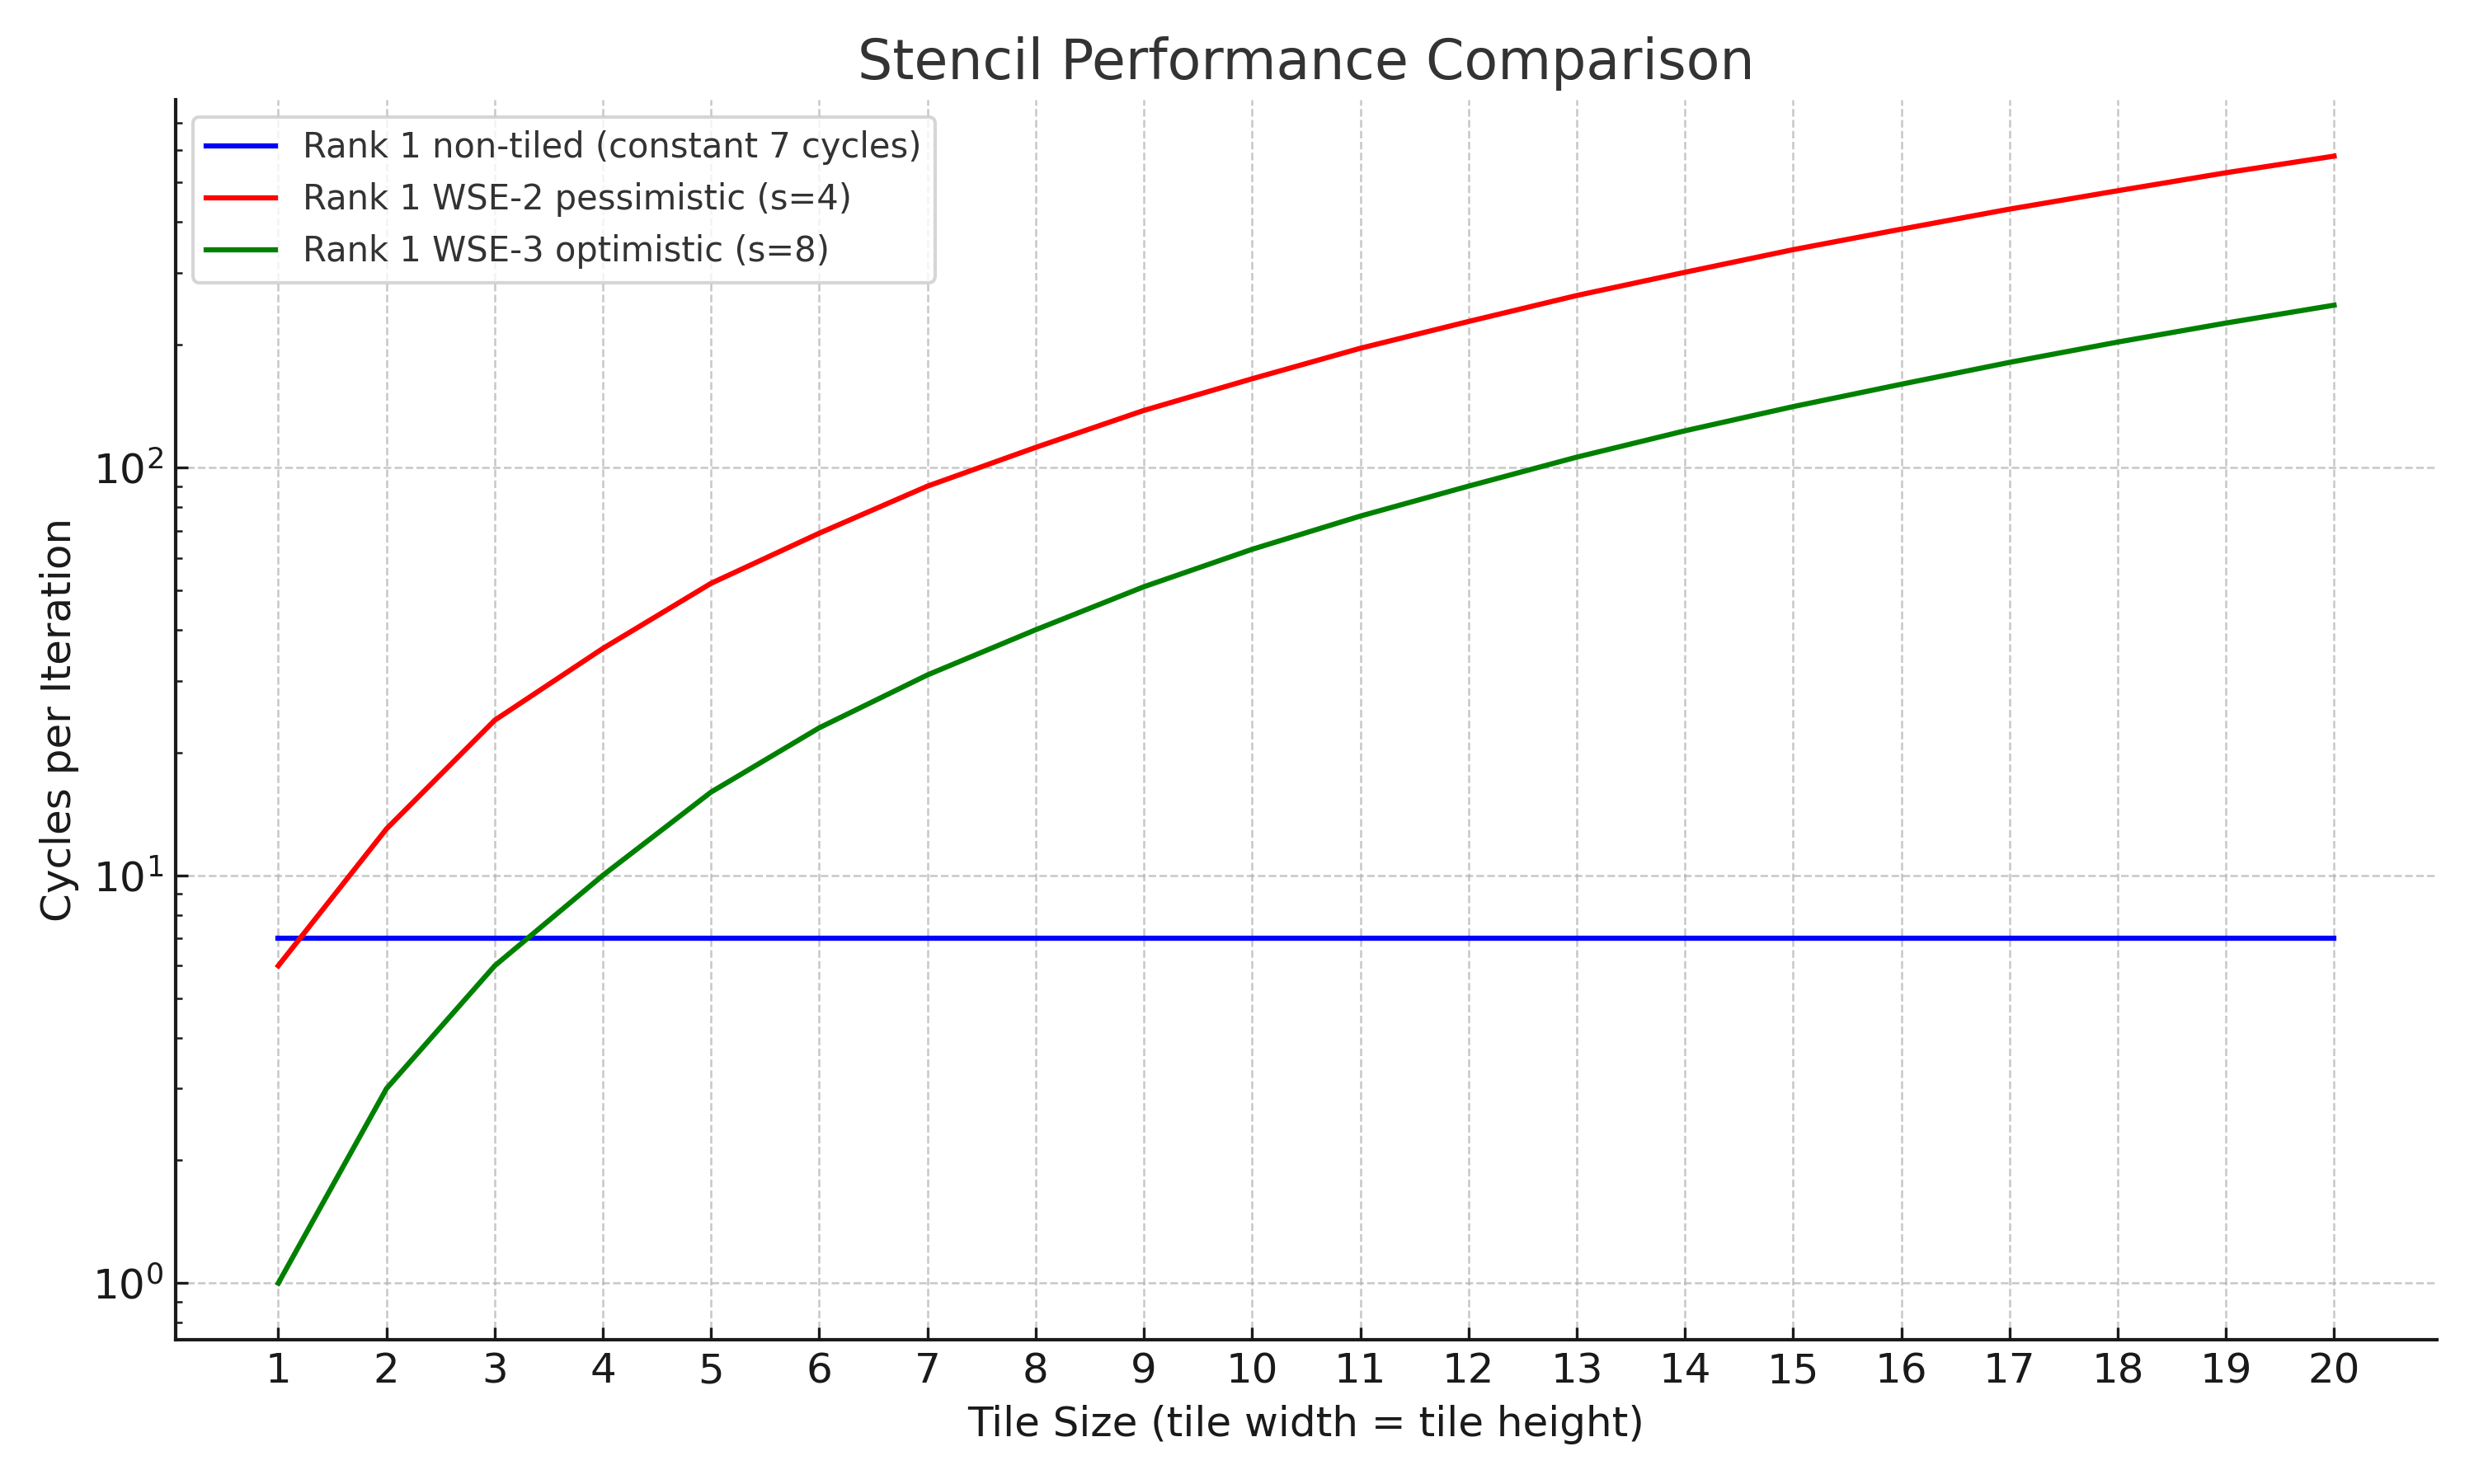
\includegraphics[width=0.5\linewidth]{stencil_performance_comparison.png}
    \caption{Cycles per iteration for tiled and non-tiled stencils theoretical performance with radius 1 }
    \label{fig:enter-label}
\end{figure} 
\chapter{Experiments}
\label{sec:experiments}
We did several experiments to answer the following questions:
\begin{enumerate}
    \item How stable is the cycle count per iteration?
    \item Is there any overhead for more \acp{pe}?
    \item When using a fixed grid size, how does the performance of using more \acp{pe} compare to using larger tiles on fewer \acp{pe}?
    \item What is the maximum tiling size that fits into the memory of a \ac{pe}?
    \item How does the performance of the generalized algorithm compare to the specialized algorithm for radius 1?
    \item How does the Cerebras implementation compare to highly optimized implementations on traditional \ac{hpc}-Arcitectures (\ac{cpu}, \ac{gpu})?
    \item What percentage of the peak performance is achieved for different tile sizes and radii?
    % \item What contributes to the cycle count?
\end{enumerate}

All experiments are performed on the cycle accurate simulator that is part of the Cerebras \ac{sdk} of which we used the version 1.3.0.
Using the simulator limits the number of \acp{pe} and number of iterations so that the data needs to be extrapolated to the whole grid.
We examine to what extend extrapolation is possible in the first two experiments.

We count the cycles used per iteration in the simulator and use this together with the clock speed of the \ac{wse} to calculate the time per iteration.

One difference between the simulator and the real hardware is that the simulator does use a single clock for all cores, while the real hardware has a separate clock for each core. (verify this!!!) Because these clocks are not perfectly synchronized, especially experiments with a large number of \acp{pe} could differ in the cycle count. Although this is not guaranteed for our algorithm, (source) find that in practice the slighly desynchronized clocks improve overall performance compared to the simulator. 

\section{Stability of cycle count per iteration}
For this experiment, we fix the grid size, tile size and radius and run the simulation for different number of iterations.
After two iterations of varying cycle count, the cycle is mostly stable.
For a grid size of 10x10, the cycle count per iteration is $16\pm1$ on \ac{wse}-2 and $23\pm1$ on \ac{wse}-3.

For a grid of 10x10, and a tile size of 1x1 and radius 1, the tiled algorithm achives $127\pm0$ cycles per iteration on \ac{wse}-2 and $156\pm1$ cycles per iteration on \ac{wse}-3.

A larger problem size with a grid of 100x100, tile size of 10x10 and radius 5, results in a cycle count per iteration of $3353\pm20$ on \ac{wse}-2 and $3377\pm5$ on \ac{wse}-3.

Because of the high flucuations in the cycle count in the first two iterations, we measure the cycle count in the following experiments as an average of the 3rd and 4th iteration.

\begin{figure}[h]
    \centering
    \begin{subfigure}[b]{0.48\textwidth}
        \centering
        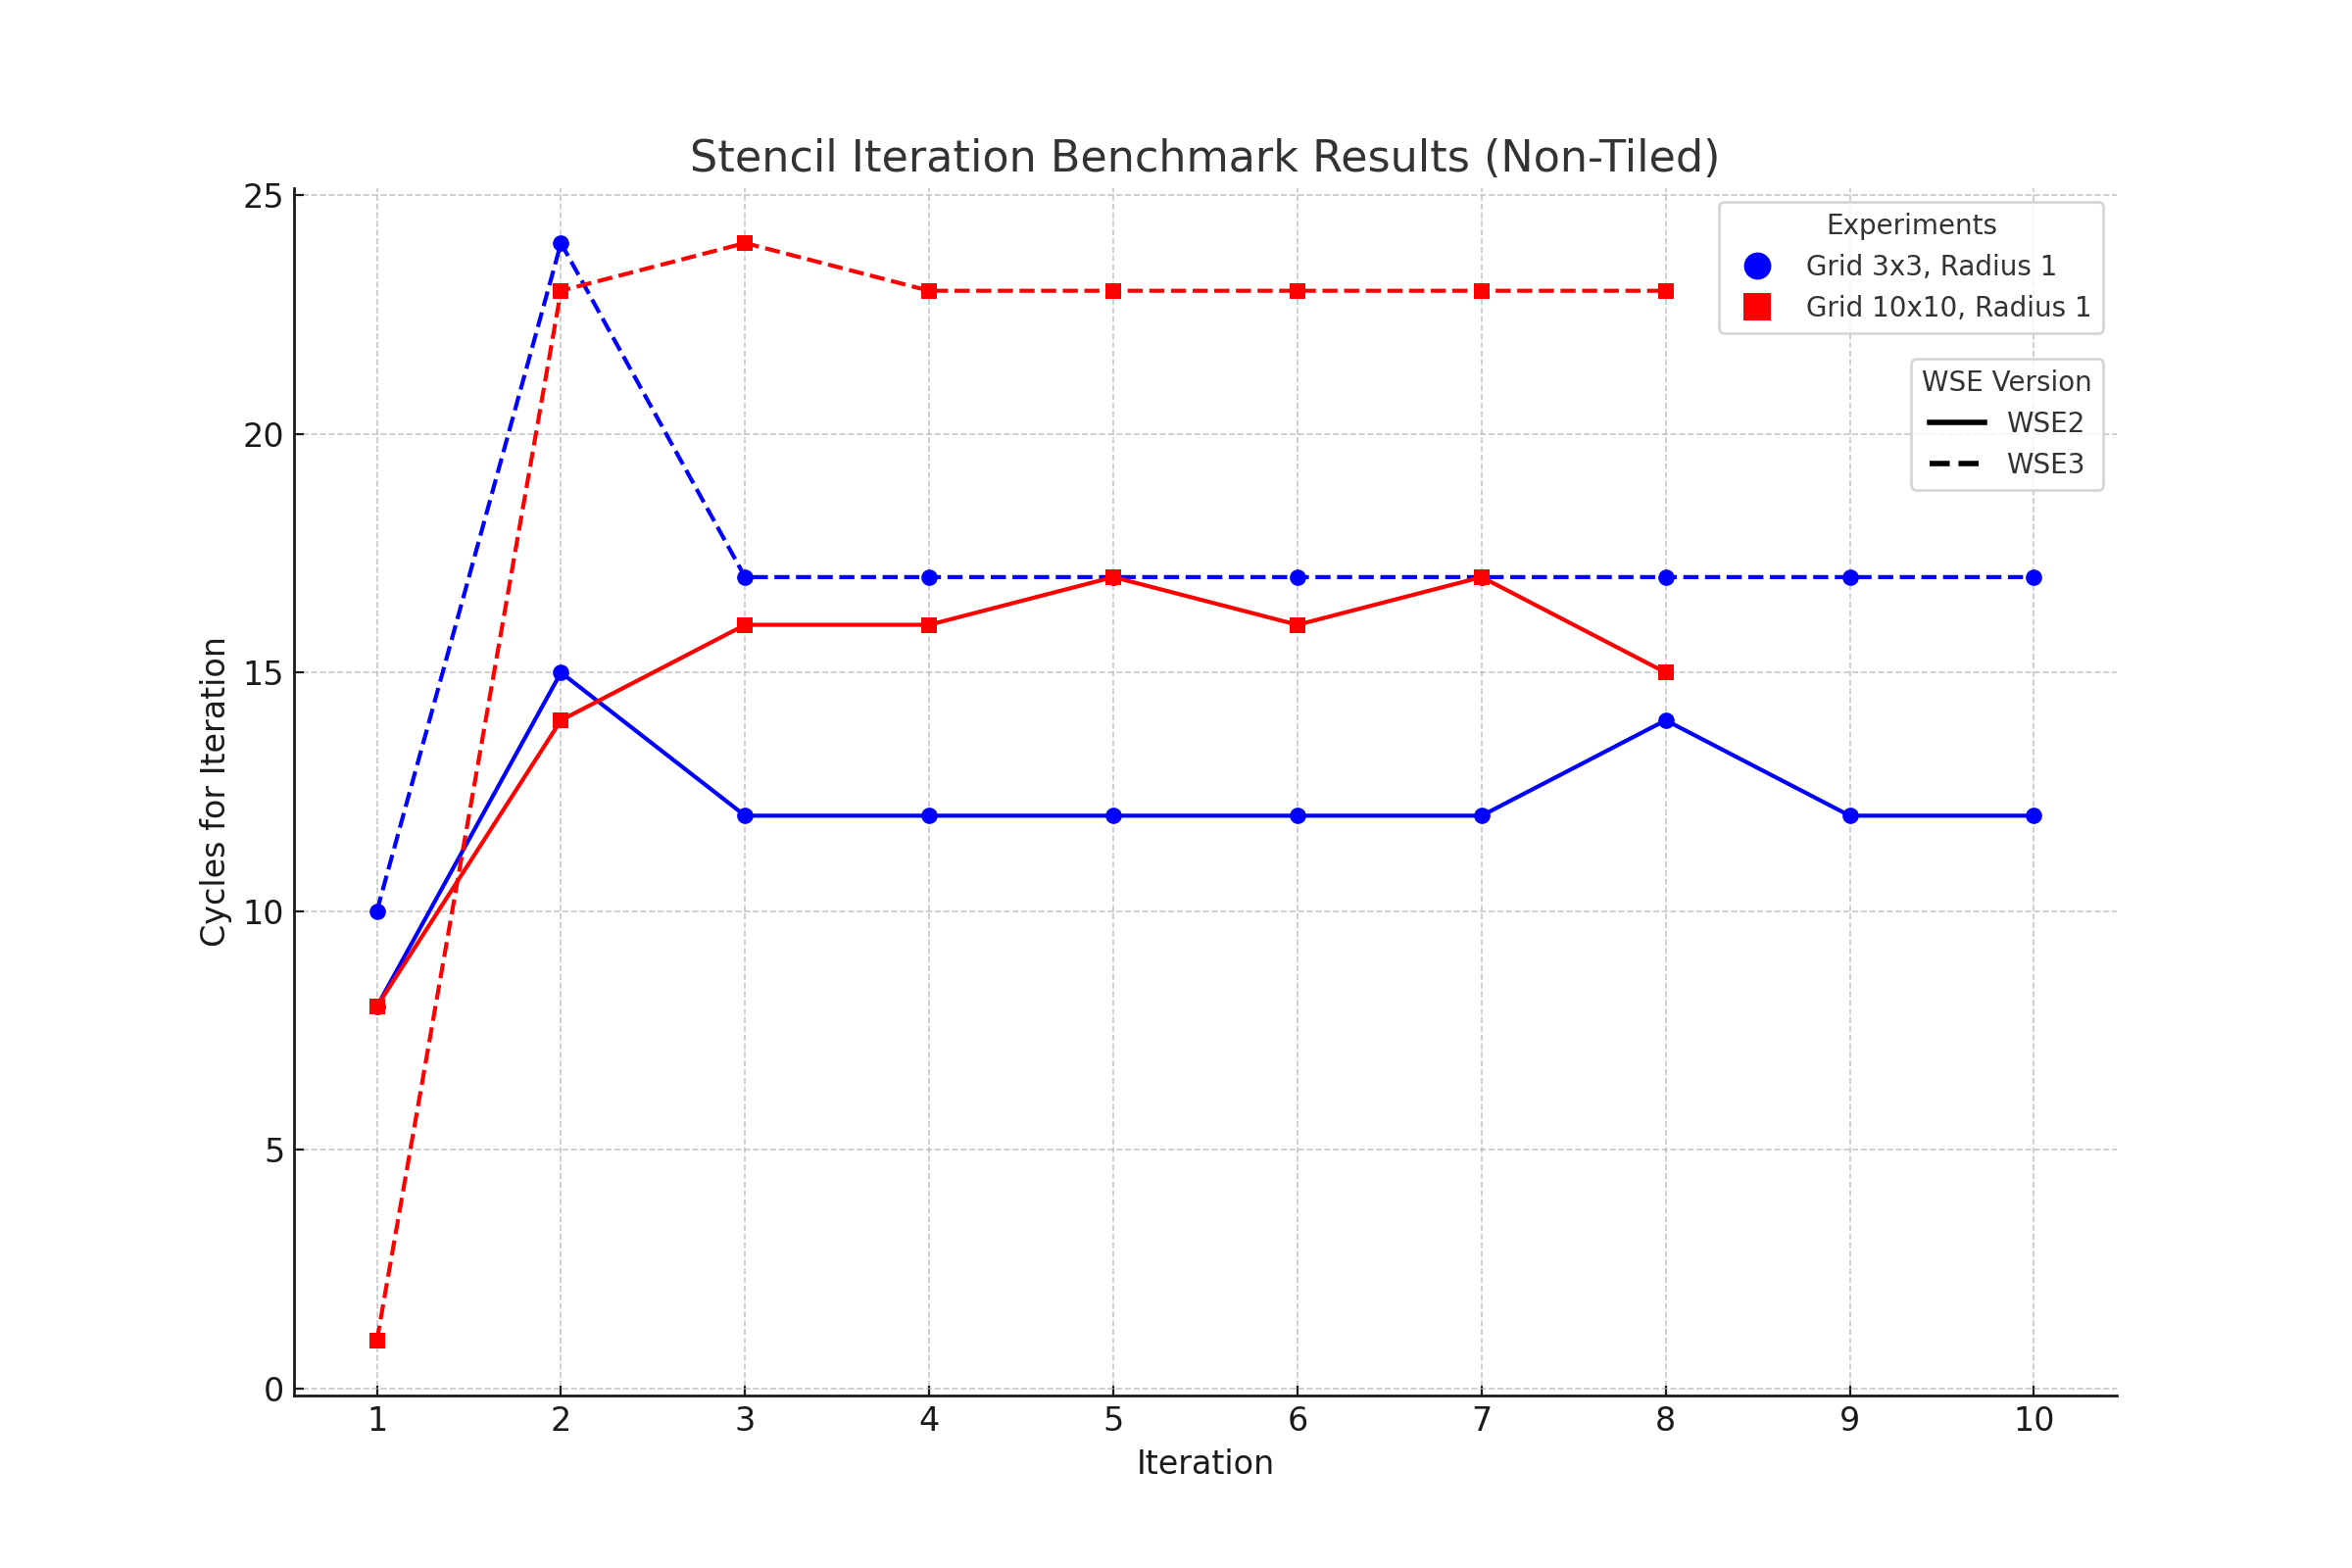
\includegraphics[width=\textwidth]{non_tiled_iteration_stability.png}
        \caption{Non-tiled algorithm}
        \label{fig:non_tiled_iteration_stability}
    \end{subfigure}
    \hfill
    \begin{subfigure}[b]{0.48\textwidth}
        \centering
        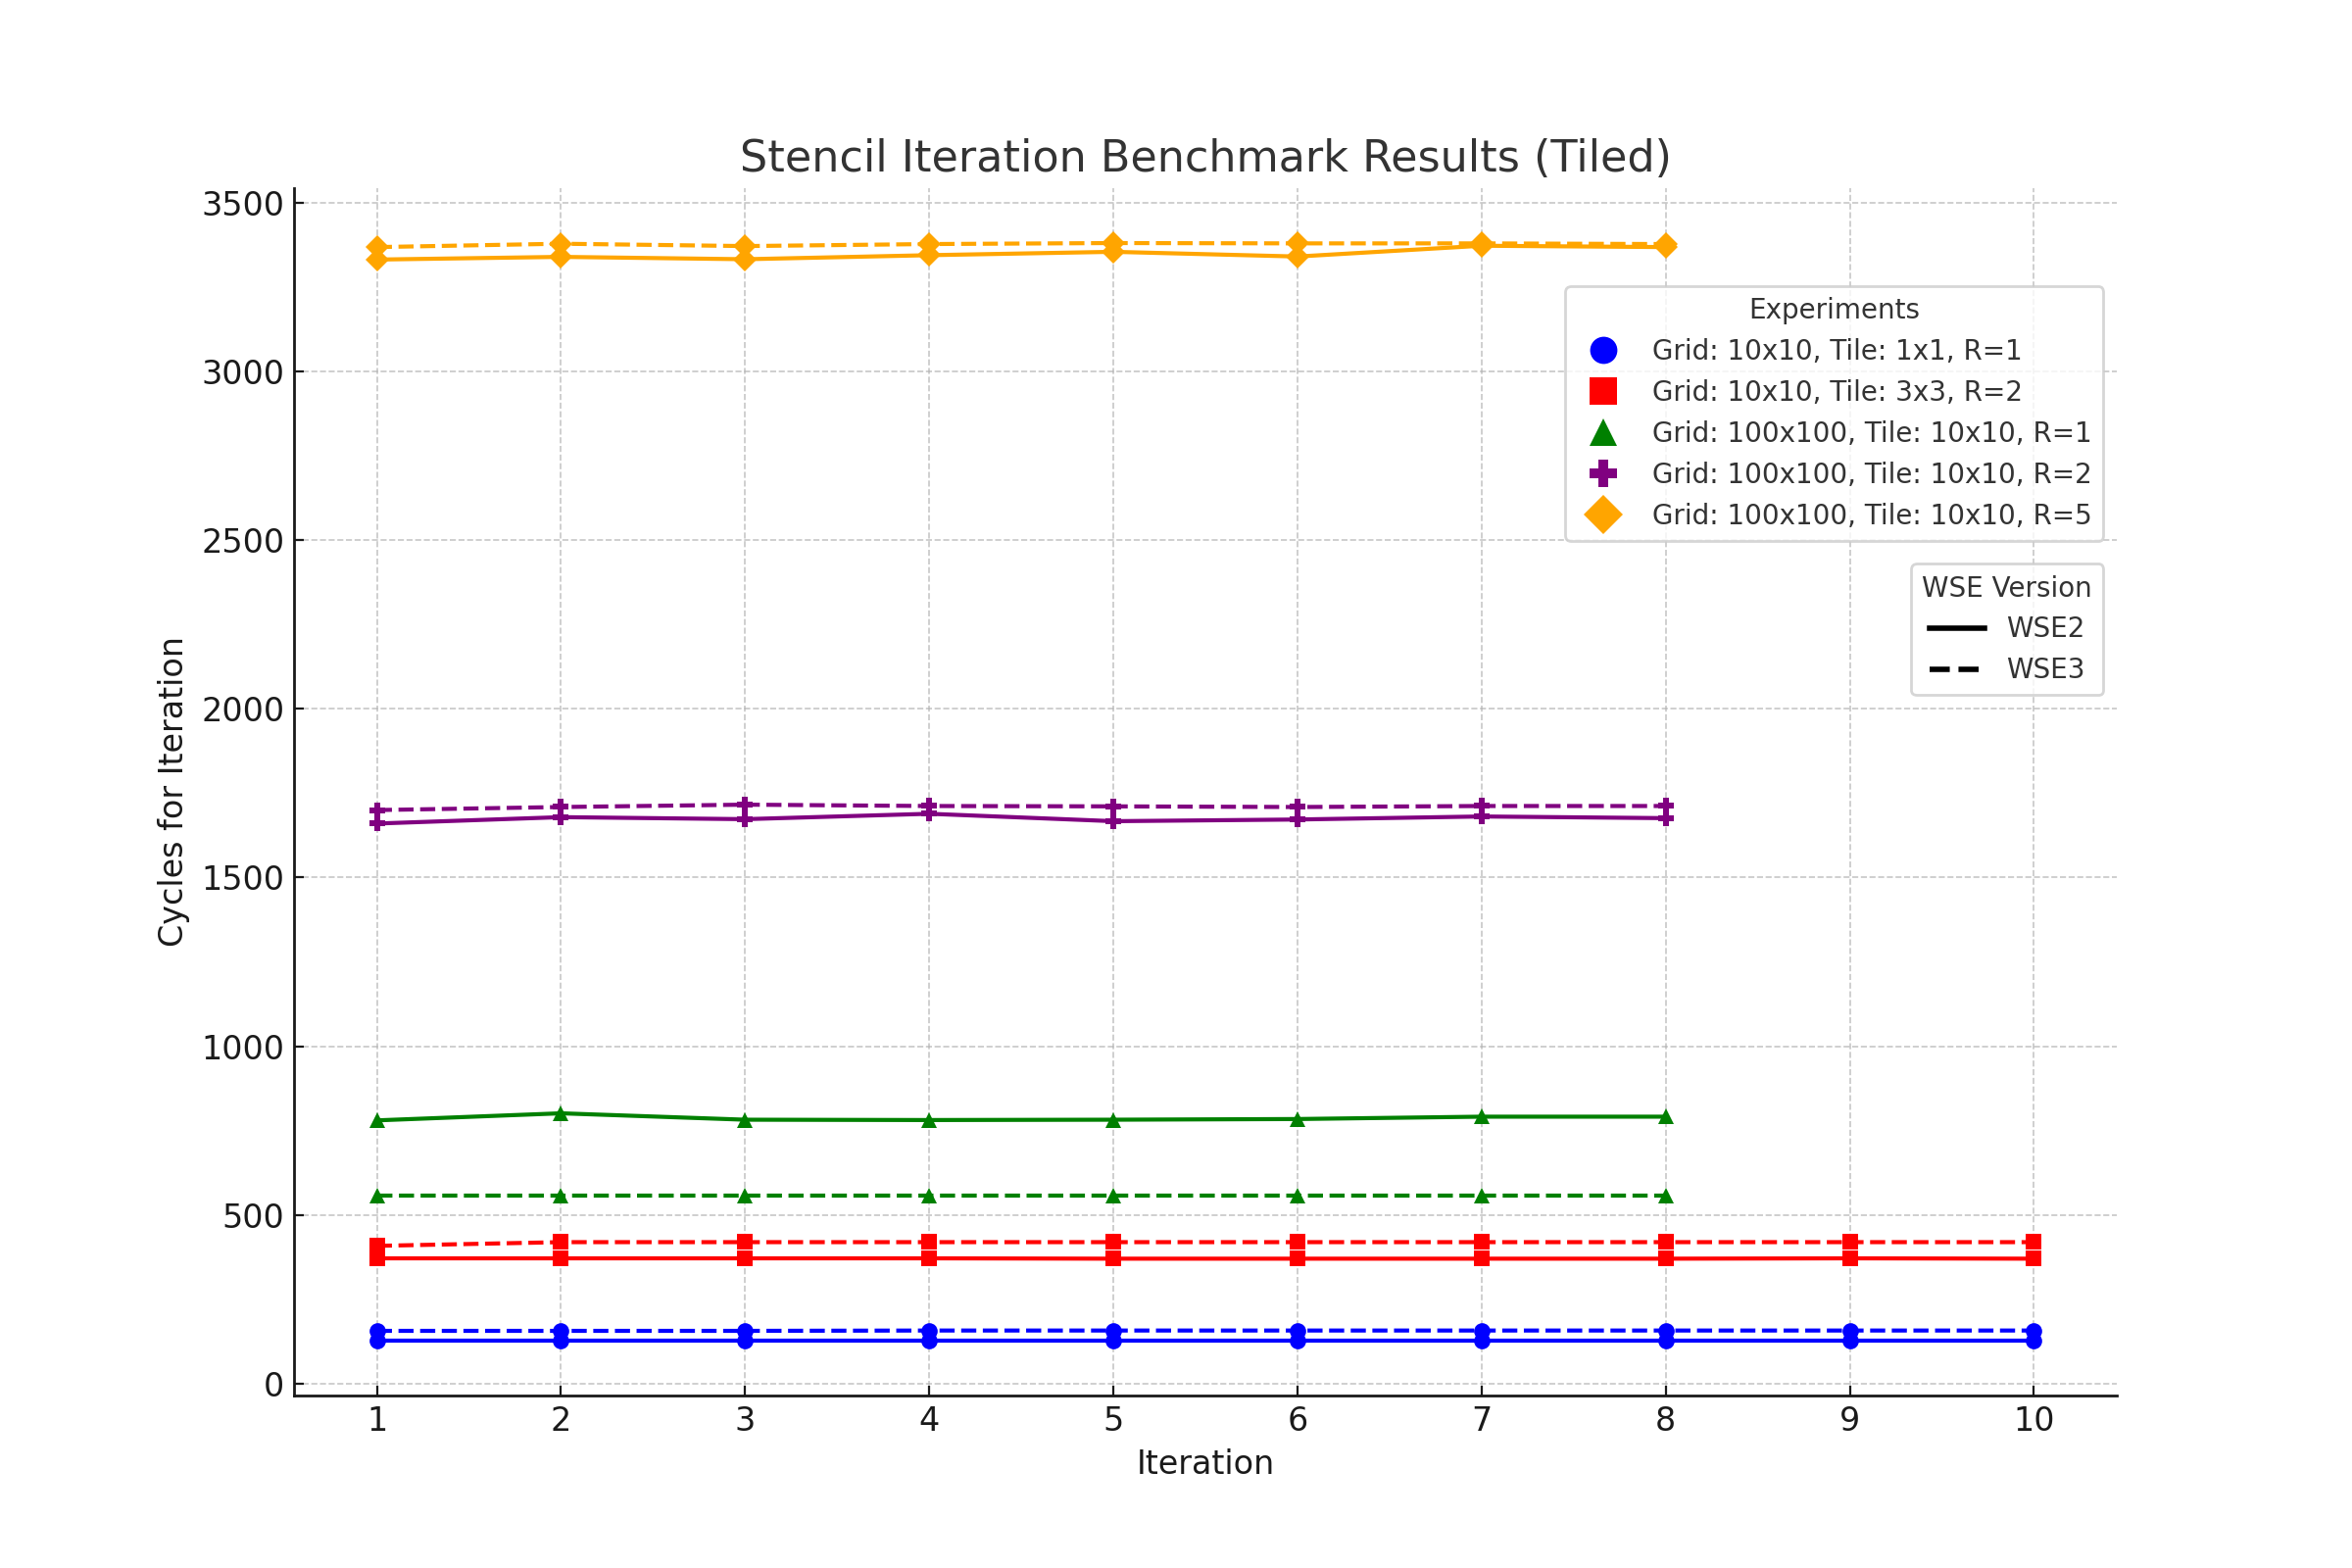
\includegraphics[width=\textwidth]{tiled_iteration_stability.png}
        \caption{Tiled algorithm}
        \label{fig:tiled_iteration_stability}
    \end{subfigure}
    \caption{Cycle count per iteration for non-tiled and tiled algorithm}
    \label{fig:iteration_stability}
\end{figure}



\section{Overhead for more \acp{pe}}
\label{sec:pe_overhead}
A very interesting question is how the performance scales with the number of \acp{pe}.
As each \ac{pe} is independent from the others, the time per iteration should be independent from the number of \acp{pe}.
This can be confirmed by the tests on the simulator up to a \ac{pe} count of \num{2500} (\numproduct{50 x 50}) for the non-tiled algorithm and \num{625} (\numproduct{25 x 25}) for the tiled algorithm.

\begin{figure}[h]
    \centering
    \begin{subfigure}[b]{0.48\textwidth}
        \centering
        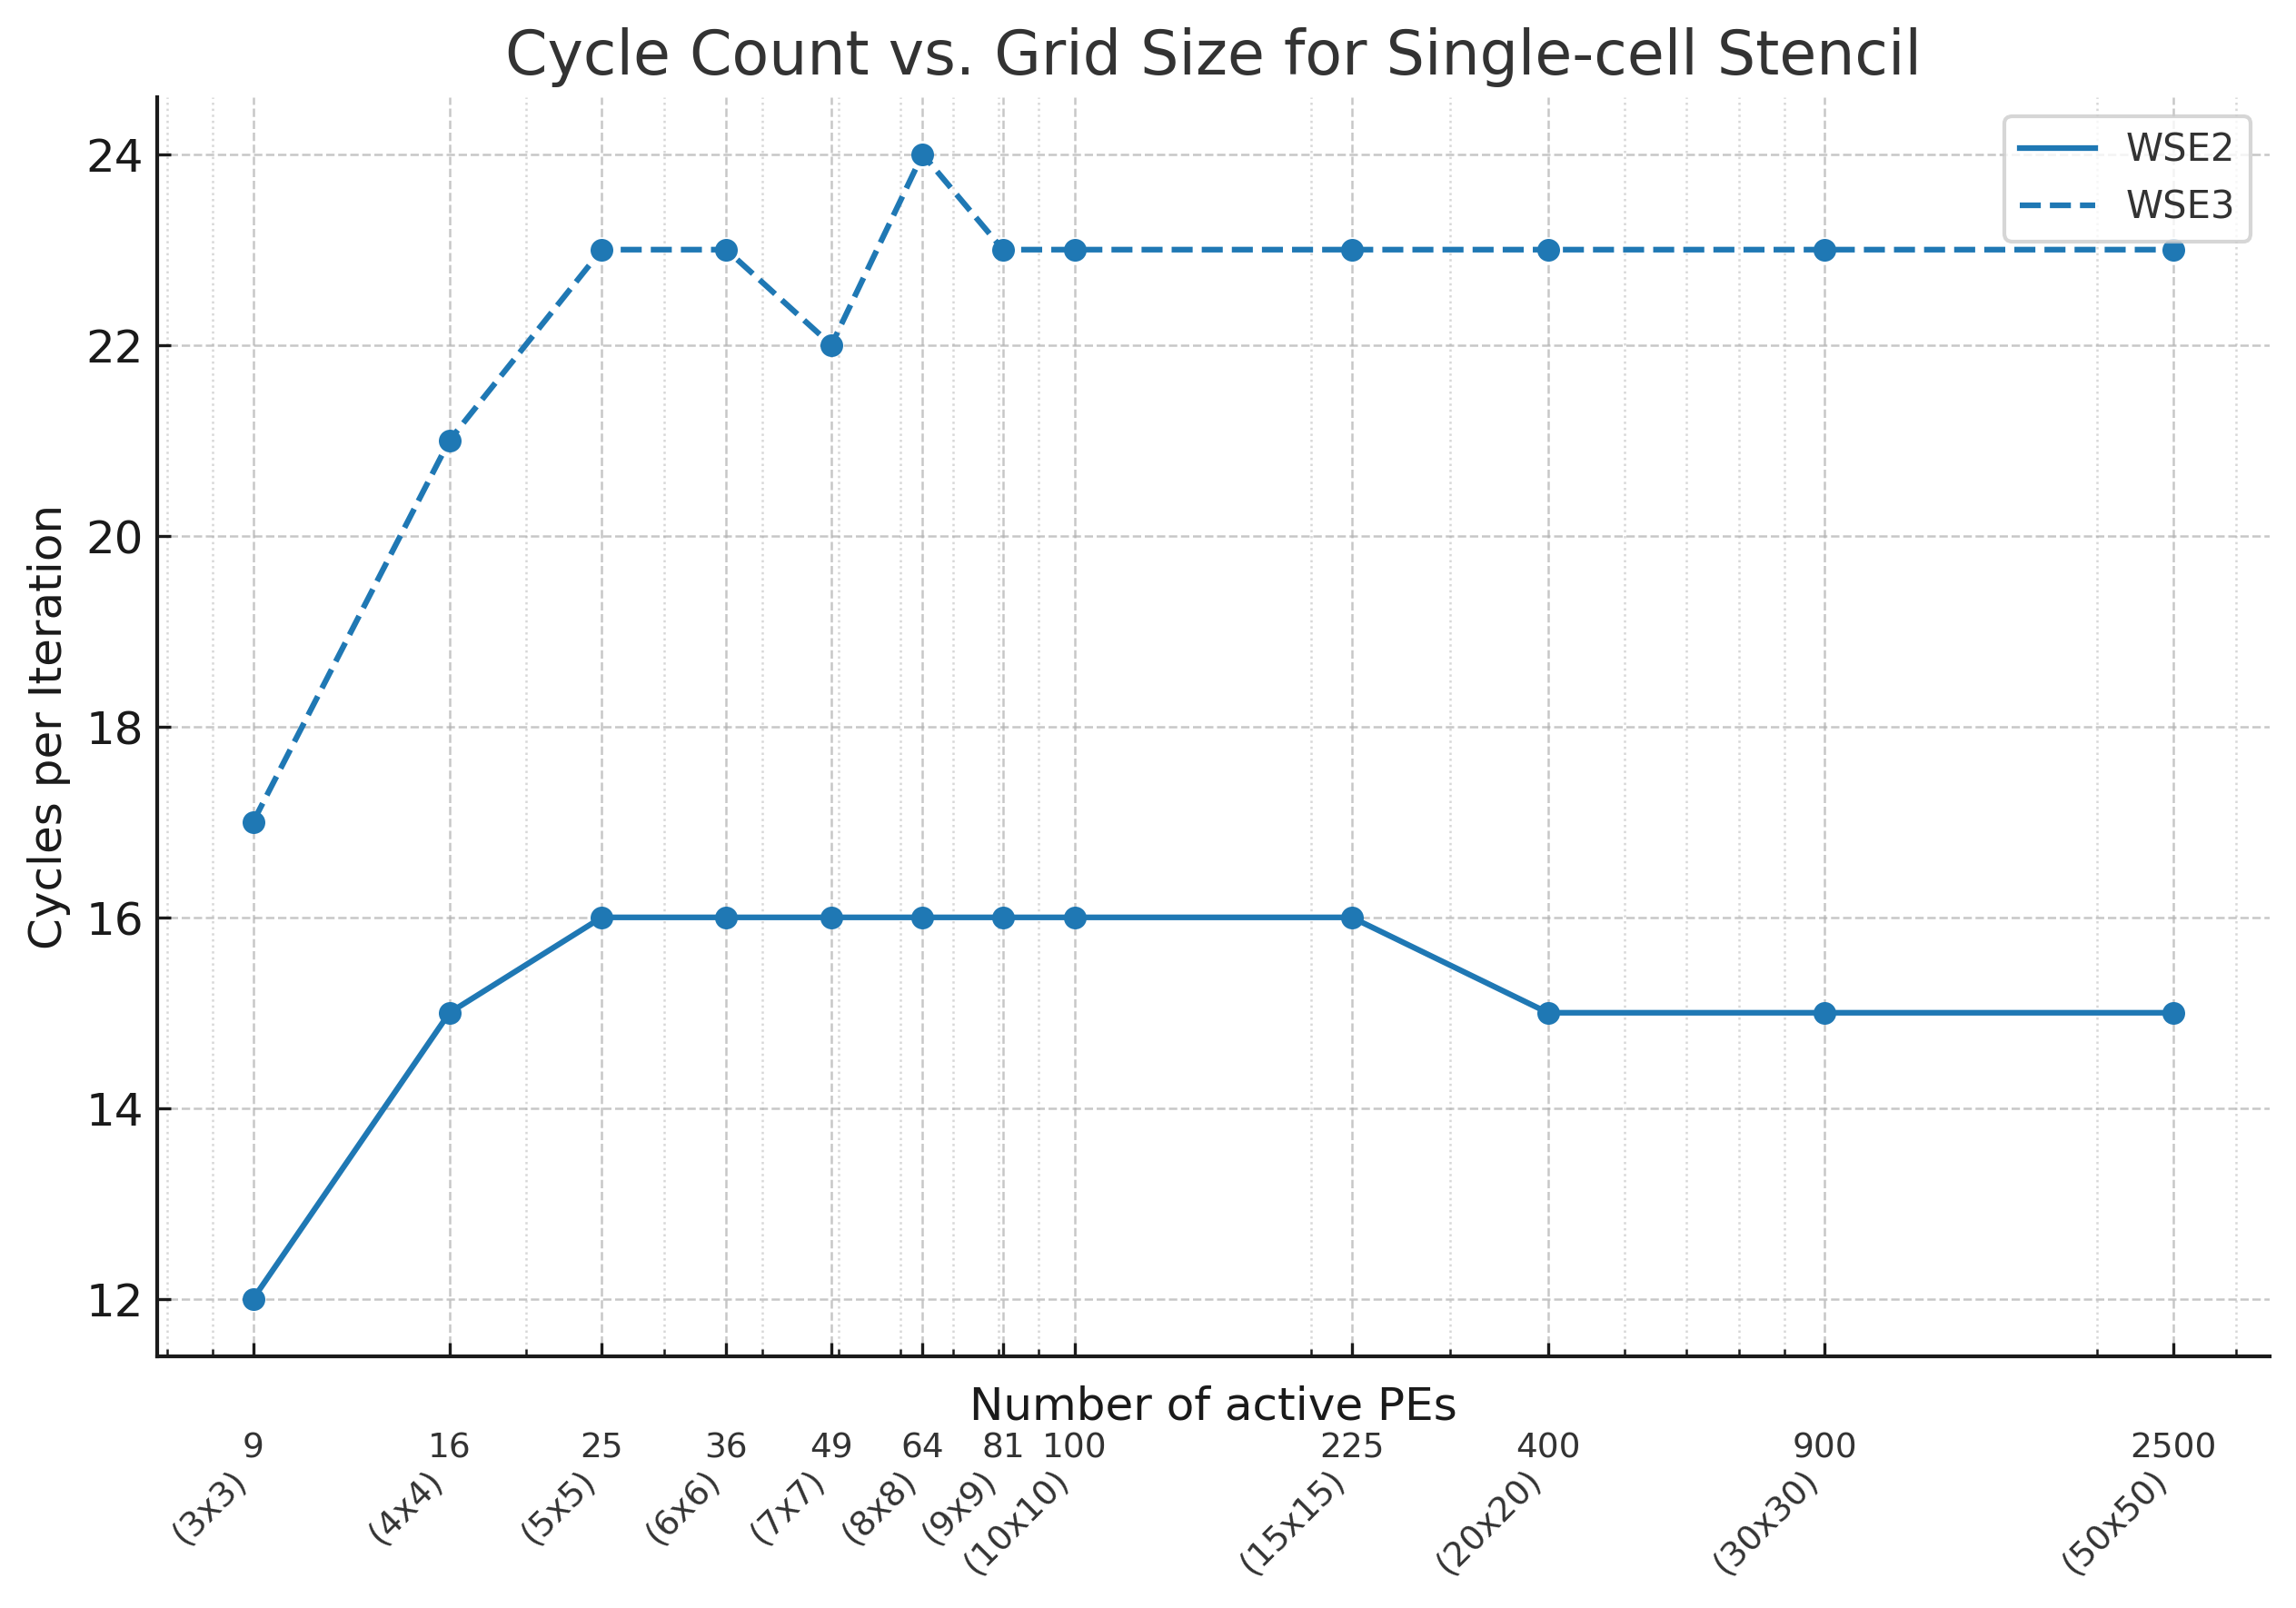
\includegraphics[width=\textwidth]{pe_overhead_non_tiled.png}
        \caption{Non-tiled algorithm}
        \label{fig:pe_overhead_non_tiled}
    \end{subfigure}
    \hfill
    \begin{subfigure}[b]{0.48\textwidth}
        \centering
        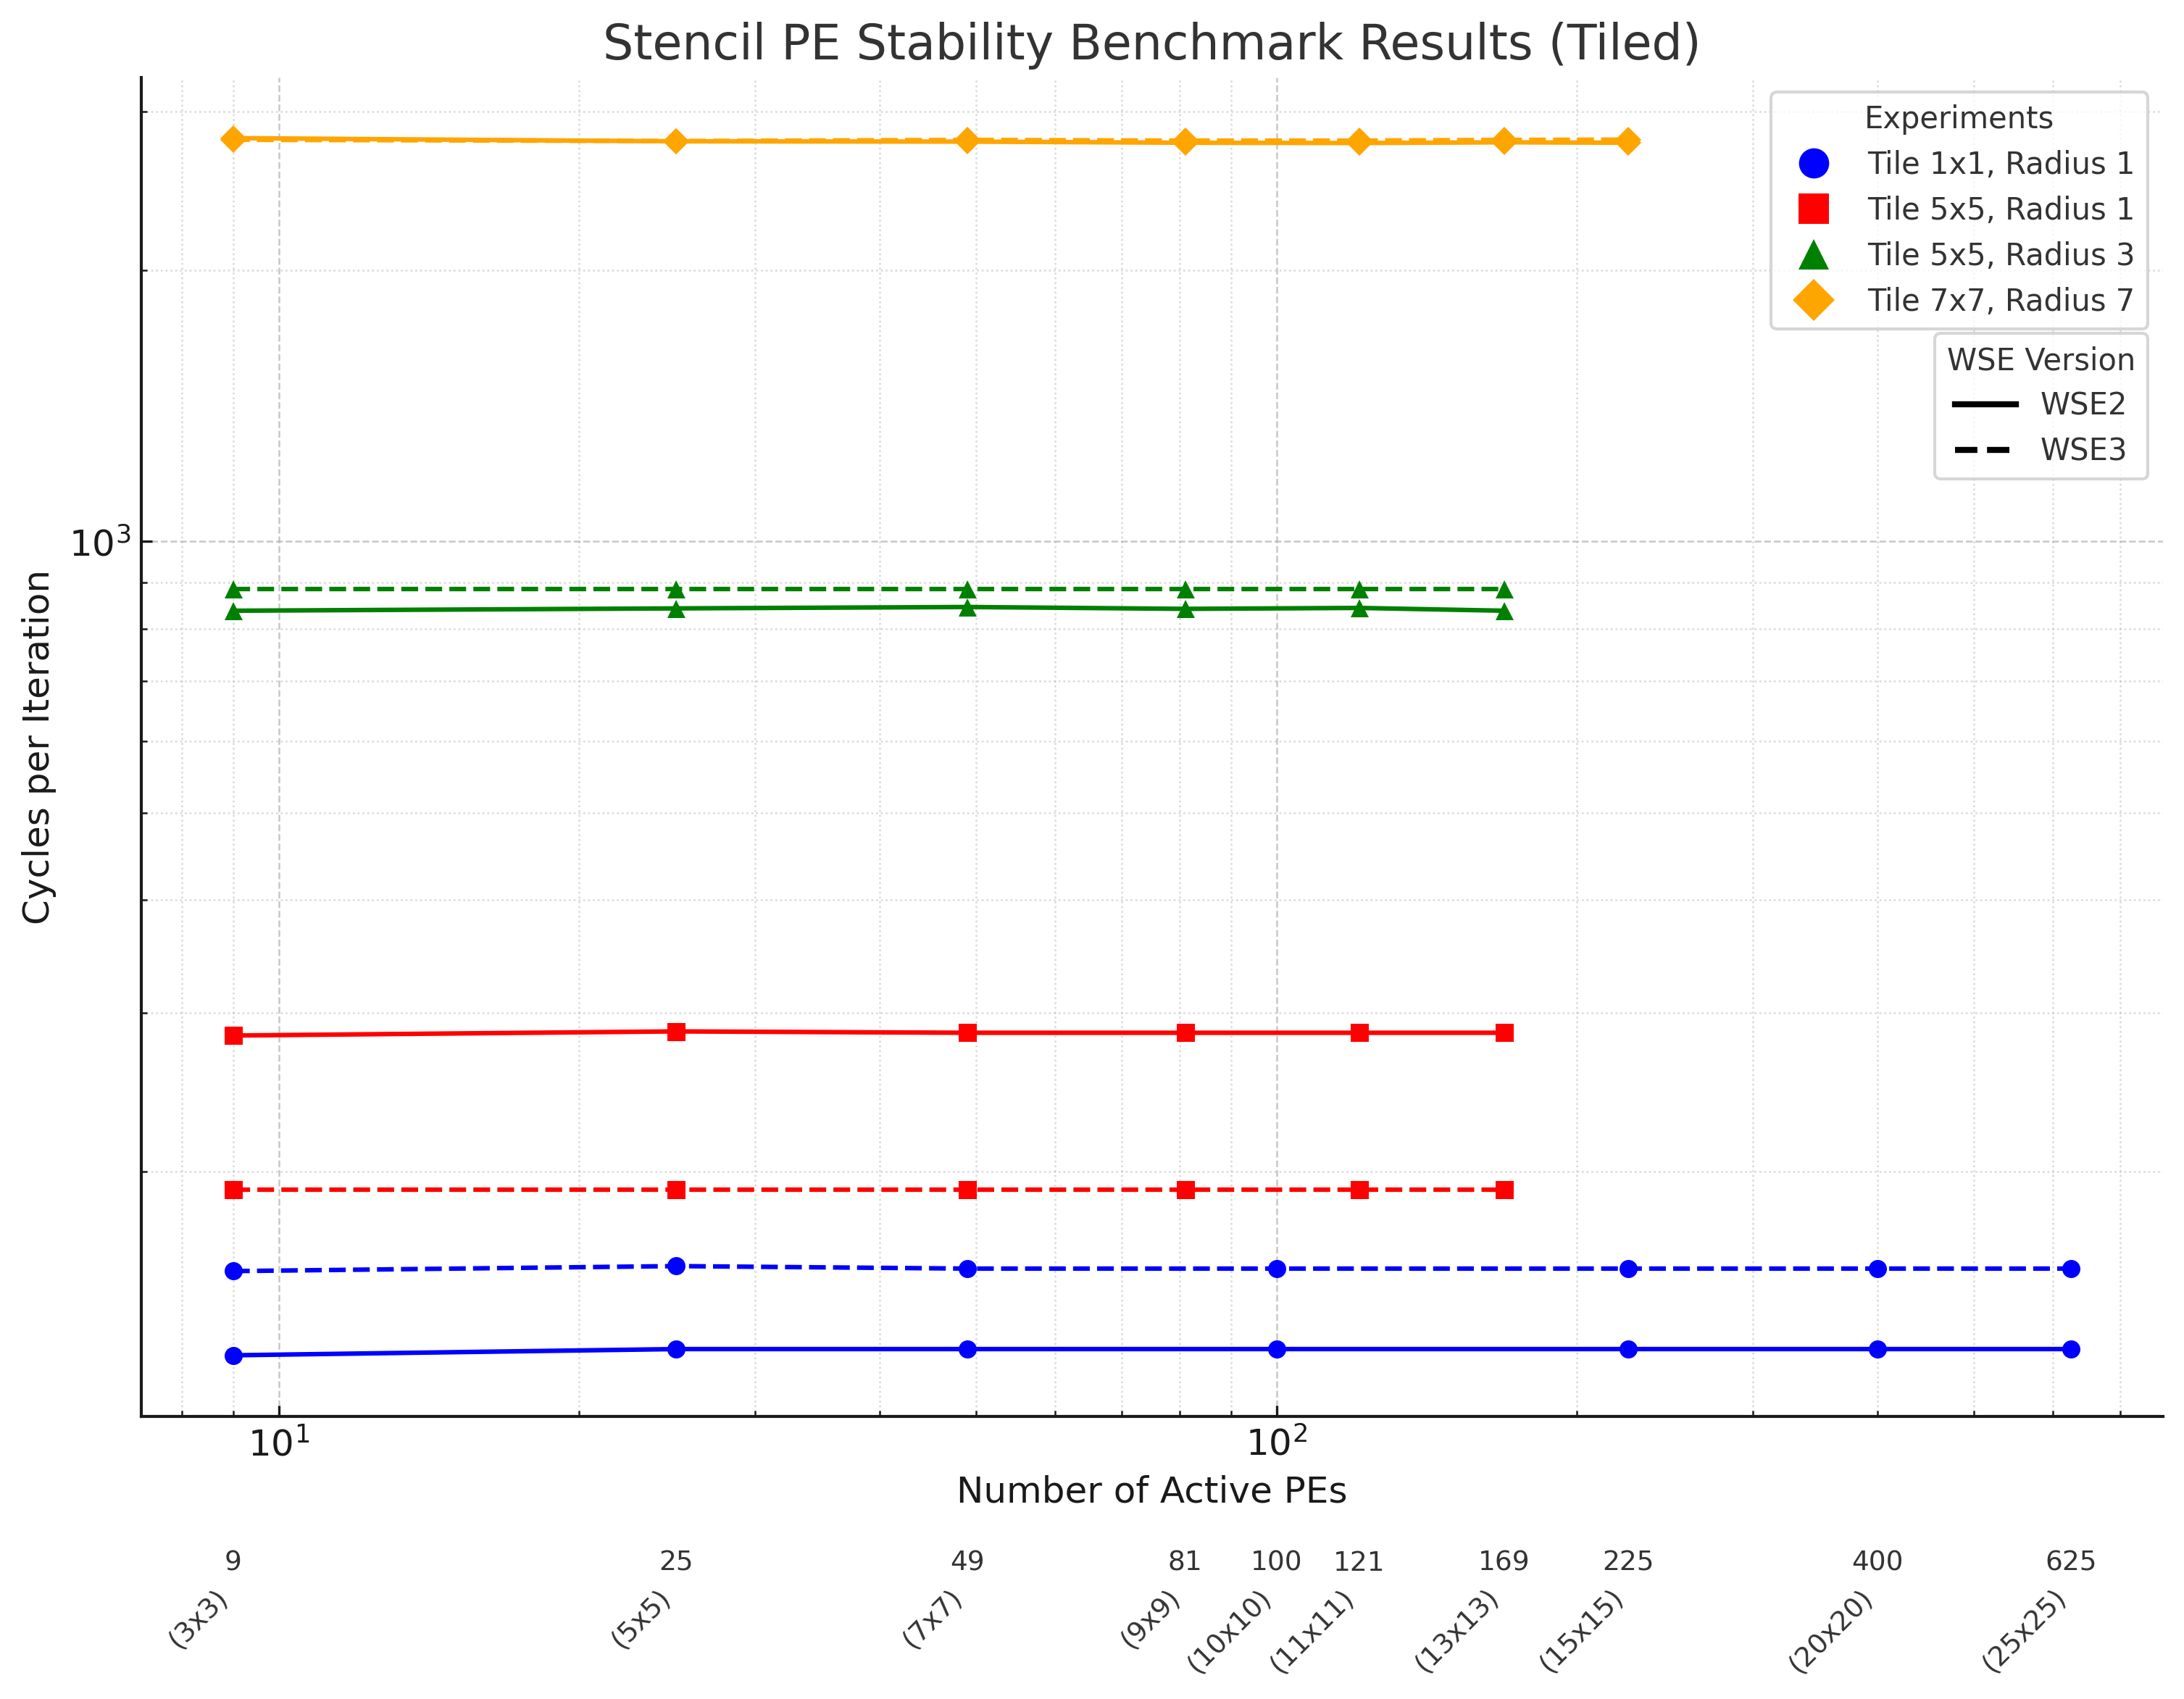
\includegraphics[width=\textwidth]{tiled_pe_stability.png}
        \caption{Tiled algorithm}
        \label{fig:tiled_pe_stability}
    \end{subfigure}
    \caption{Cycle count per iteration versus the number of active PEs for (a) the non-tiled algorithm and (b) the tiled algorithm. For the non-tiled implementation, the performance is stable for grids larger than 4x4, with the 3x3 grid showing a notably lower cycle count. The tiled implementation also demonstrates a consistent cycle count for a given configuration, independent of the number of active PEs.}
    \label{fig:pe_overhead}
\end{figure}

As shown in \autoref{fig:pe_overhead_non_tiled}, the performance of the non-tiled algorithm scales almost perfectly, with the cycle count remaining constant with minimal fluctuations regardless of the grid size. The one exception is the 3x3 grid, which is significantly faster. We hypothesize this is an artifact of the experimental setup where only the single, inner \ac{pe} is performing computation and does not need to synchronize with other computing neighbors, effectively eliminating the communication latency discussed in \autoref{sec:theoretical_performance_evaluation_and_comparison_against_roofline_model}. For all subsequent experiments, we ensure at least \numproduct{5 x 5} active \acp{pe} - which results in at least \numproduct{3 x 3} \acp{pe} inner \acp{pe} - to provide representative results.

Jacquelin et al. \cite{jacquelin2022massively} show that for a 3d stencil that is tested on real hardware, the cycle count scales almost perfectly with the number of \acp{pe} up to the whole \ac{wse} dimensions.
We therefore expect that our implementation also scales nearly perfectly on the real hardware and calculate with this assumption in the following experiments.

\section{Maximum tiling size}
The maximum tiling size that fits into the memory of a \ac{pe} is limited by the number of memory banks and the size of the data structure registers.
We test this by increasing the tile size to the maximum that still compiles for (test wse2 and wse3 independently!!! currently same number for both (smaller one))

We find that the maximum tiling size  is 64x64=4096 elements.
A non-quadratical tile size, that results in 4096 elements, is likely also possible, but not tested.
Tile size of 64x64 was tested up to radius 3. It is likely to decrease for larger radius.

This results in a maximum grid size containing \num{3101280000} elements on wse-2 and \num{3670474752} elements on wse-3.
Note that due to hardware limitations of the \ac{wse}, the maximum stride for \acp{dsd} is \num{127} which makes very uneven distributions between tile width and tile height not possible.


\section{Comparison of non-tiled and tiled algorithm}

The non-tiled algorithm is implemented in a completely different way than the tiled algorithm.
This allows for a very optimized implementation, that doesn't require any runtime \ac{dsd} to \ac{dsr} transfers, asynchronous operations and task activation.
It is therefore significantly faster than the tiled algorithm for radius 1.
However, the non-tiled algorithm is naturally limited to a radius of 1 and a grid size not larger than the \ac{wse} dimensions.

\begin{figure}[h]
    \centering
    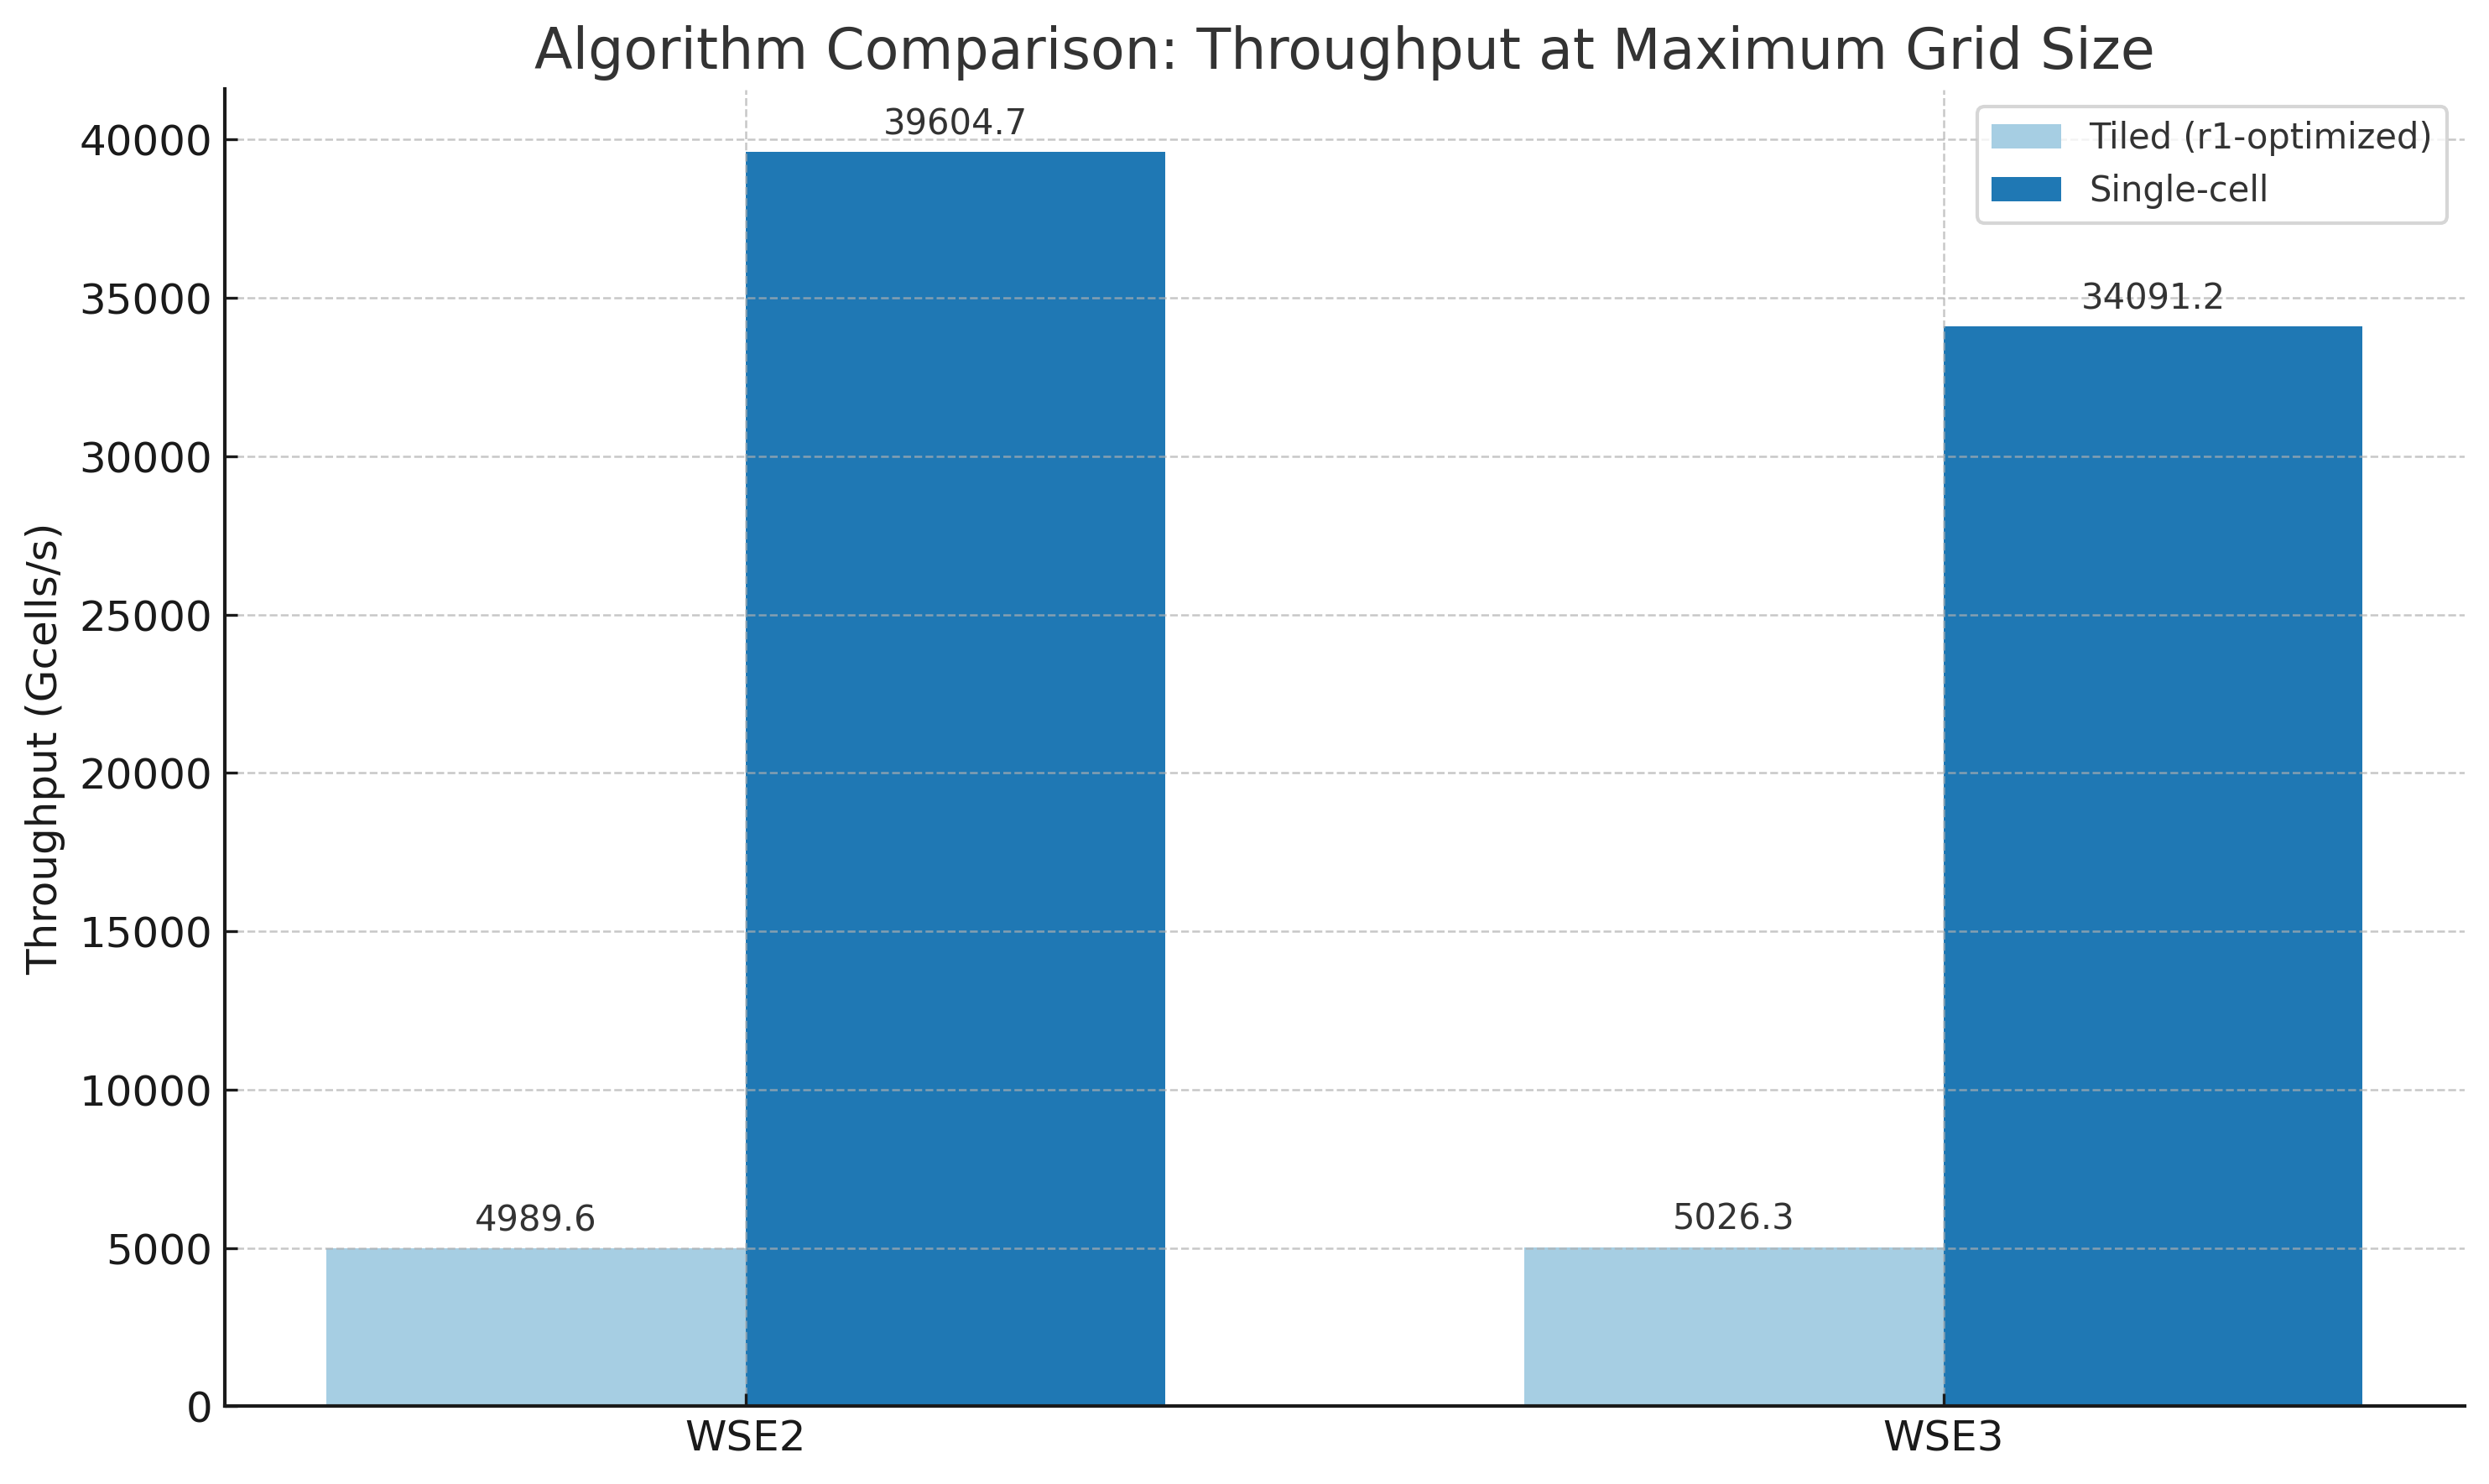
\includegraphics[width=0.5\linewidth]{algo_comparison.png}
    \caption{Performance comparison of the specialized non-tiled and the r1-optimized tiled implementations for a radius-1 stencil. The specialized, non-tiled algorithm is significantly faster, achieving an 8x speedup on \ac{wse}-2 and a 7x speedup on \ac{wse}-3 due to its simpler communication and execution model.}
    \label{fig:algo_comparison}
\end{figure}

\section{Comparison of Cerebras and traditional \ac{hpc}-Arcitectures}
We conducted two more experiments to compare the performance of the implemented stencil on the Cerebras \ac{wse} with highly optimized Devito implementations for \ac{cpu} and \ac{gpu}. The experiments were conducted using the Vast.ai cloud.
For the \ac{cpu} experiments we used a system with two AMD EPYC 9554 64-Core processors. The system has a total of \qty{128}{\mega\byte} of L2 cache and \qty{512}{\mega\byte} of L3 cache. It is equipped with \qty{1511}{\giga\byte} of DDR5 memory.
The system is furthermore equipped with a NVIDIA H100 SXM 80GB, which was used for the \ac{gpu} experiments. The system had CUDA 12.8 installed and we used python 3.12.11, Devito 4.8.19, Cupy 13.4.1 and the nvc compiler in version 25.5.

For each benchmark we fixed the total work load, i.e., $width\times height\times N$, so that every configuration performs the same number of stencil updates while varying only the memory footprint. Steady-state performance was obtained by first running an untimed warm-up of $N$ iterations (triggering JIT compilation, allocations and data transfers) and then timing a second run of the same $N$ iterations with all data already resident on the \ac{cpu} or \ac{gpu}. This was done for grids with a total size of $10^x$ for $x \in \{4..9\}$ and radii in \numrange{1}{6}.
The compute work, while in this experiment constant for different grid sizes, rises linearly with the radius, which on the other hand has no significant effect on memory footprint.
Furthermore, we calculated the neccessary tile size to fit the same grid sizes on the \ac{wse}-3 and ran an experiment with this tile size for radii \numrange{1}{6} and a total grid size that results in \numproduct{5 x 5} active \acp{pe} in the simulator for four iterations and took the average cycle count of the last two iterations.
Assuming perfect scaling accross the WSE as suggested by the results from \autoref{sec:pe_overhead}, we used this cycle count together with the \ac{wse}s clock frequency to calculate the theoretical throughput when using the entire \ac{wse} dimensions.
We also added the throughput, the non-tiled algorithm would achieve on the \ac{wse}-3 where the \ac{wse}-3s hardware dimensions allow for the grid size.
As the $width$ and $height$, we strictly used powers of 10, resulting in rectangular grids for odd $x$.
To have all experiments use \numproduct{5 x 5} active \acp{pe} in the simulator, we used a grid size of $\roundbrack{3\times t_w + 2r, 3\times t_h + 2r}$.

To ensure the entire problem grid fits onto the available number of \acp{pe}, the tile size ($t_w$, $t_h$) for a given grid of size ($G_w$, $G_h$) on a \ac{wse} with physical dimensions ($P_w$, $P_h$) is determined by:
\begin{equation}
    t_w = \left\lceil \frac{G_w}{P_w} \right\rceil, \quad t_h = \left\lceil \frac{G_h}{P_h} \right\rceil
\end{equation}

For example, to map the \numproduct{10e3 x 10e4} grid onto the \ac{wse}-3 with its \numproduct{762 x 1176} \acp{pe} array, we calculate the tile size. Mapping the grid's width to the \acp{pe} array's width results in a tile width of $\left\lceil \frac{1000}{762} \right\rceil = 2$ and a tile height of $\left\lceil \frac{10000}{1176} \right\rceil = 9$. However, mapping the grid's width to the \acp{pe} array's height is more efficient, yielding a tile width of $\left\lceil \frac{1000}{1176} \right\rceil = 1$ and a tile height of $\left\lceil \frac{10000}{762} \right\rceil = 14$. To minimize the total tile area and therefore the per-\ac{pe} workload, we chose the smaller configuration of $1 \times 14$. It is important to note that due to the radius constraint from \autoref{eq:radius_constraint}, the shorter dimension of the tile must be at least as large as the radius, so the effective tile size was adjusted accordingly if necessary.

\begin{table}[h]
    \centering
    \caption{Final parameters for the experiment in the simulator for a grid size of \num{1e7}}
    \begin{tabular}{ll}
        \hline
        Parameter & Value \\
        \hline
        Grid size & \numproduct{5 x 44} \\
        Tile size & \numproduct{1 x 14} \\
        Radius & \num{1} \\
        Number of iterations & \num{2} and \num{4} \\
        \hline
    \end{tabular}
    \label{tab:sim_params}
\end{table}

\begin{figure}[h]
    \centering
    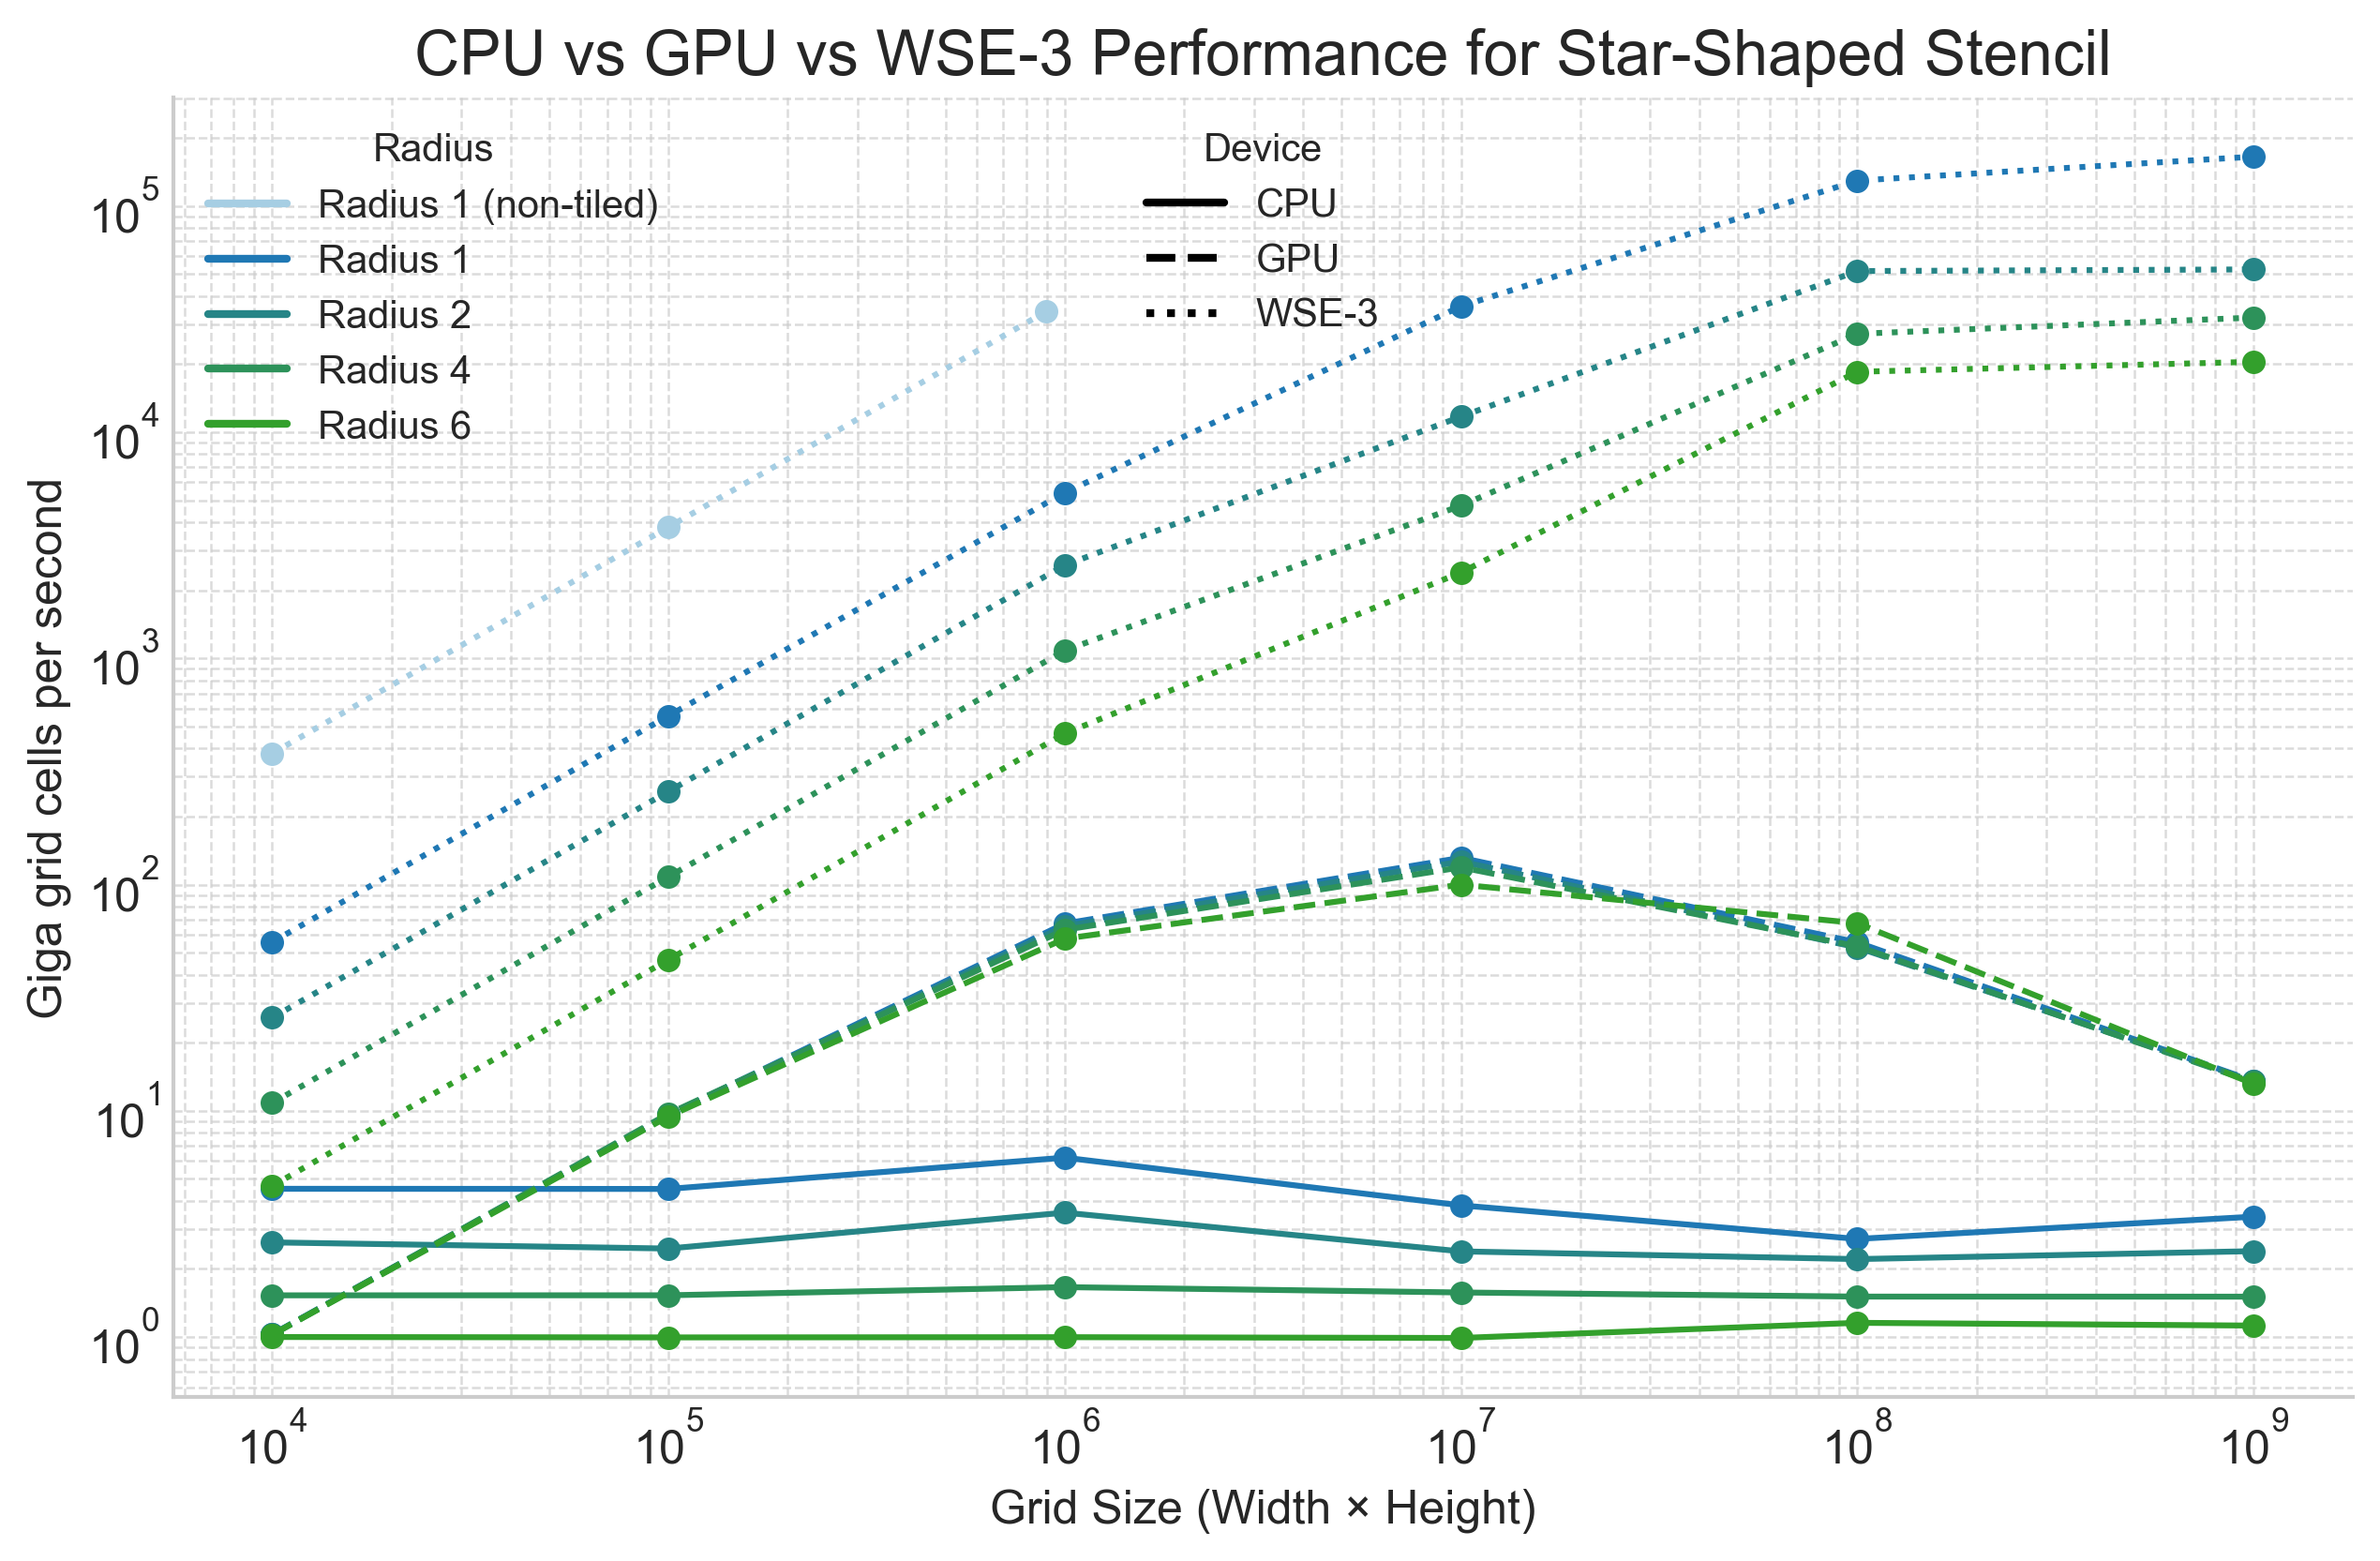
\includegraphics[width=1\linewidth]{gpu_cpu_wse3_constant_product_gcells.png}
    \caption{Comparison of \ac{cpu}, \ac{gpu} and \ac{wse}-3 performance in Giga-cells per second (Gcells/s) for different grid sizes and radii.}
    \label{fig:gpu_cpu_constant_product}
\end{figure}

The results, shown in \autoref{fig:gpu_cpu_constant_product}, show that the \ac{cpu}'s throughput is very insensitive to the work allocation and differs only by a factor of \num{2.3} between its most efficient grid size of \num{1e6} and its least efficient grid size of \num{1e8} at a radius of 1. For the largest tested radius of \num{6} this effect is even smaller at a factor of \num{1.2}.

The \ac{cpu}s insensitivity to the work allocation suggests that it is compute limited.
This gets confirmed by the fact that the \ac{cpu} throughput scales almost inversely with the radius. For the \ac{cpu} and its optimal grid size of $\num{1e6}$, the throughput for the radius-1 stencil is \num{6.2} times higher than for the radius-6 stencil, which is \num{6} times as computationally expensive.

Furthermore we observe that \ac{gpu} performance differs significantly depending on work allocation, with a peak throughput of \qty{131.4}{Gcells/s} for the optimal grid size of $\num{1e7}$ and a 128x lower throughput for the least efficient grid size of $\num{1e4}$. Interstingly a very large grid size of $\num{1e9}$ also results in a 9.7x lower throughput than the optimal grid size. While looking for a possible explanation for the pronounced optimum at a grid size of \num{1e7}, we find that the required memory of $\num{1e7}\times\qty{4}{\byte}=\qty{40}{\mega\byte}$ fits perfectly into \qty{50}{\mega\byte} L2 cache of the H100.
Other than the \ac{cpu}, the \ac{gpu} is very insensitive to the radius. So much that all differences in performance for different radii are more likely attributed to measurement errors than to a real difference in the runtime.
This strongly suggests that the \ac{gpu} is memory limited through all the different tested grid sizes.

The results show that for most tested configurations, the \ac{gpu} achieves higher throughput than the \ac{cpu}.
However for very small grid sizes of \numproduct{100 x 100}, the \ac{cpu} is more efficient.

The \ac{wse}-3 is very sensitive to both the work allocation and the radius. The sensitivity to radius is significant accross all grid sizes with a factor of \num{12.0} between radius \num{1} and \num{6} for a grid of \num{1e4} and factor of \num{8.1} between radius \num{1} and \num{6} for a grid of \num{1e9}.
The more than linear scaling for small grid sizes can be explained by the fact that these problems use a tile size of \numproduct{1 x 1} for radius \num{1} and \numproduct{6 x 6} for radius \num{6} which results in $r^2(10r-1)$ flops per \ac{pe}. This number rises with the cube of $r$. The 12x now appears relatively low and is caused by communication also playing a major role in the overall time for these small grid sizes. For a grid size of \num{1e9} on the other hand, the tile size is constant for all radii and the scaling is closer to linear with an outlier for radius \num{1}, because this uses the $r1$ optimized tiled algorithm. The factor between radius \num{2} and \num{6} is \num{2.6}.

Analyzing the \ac{wse}-3s performance, we find that the iterations per second is constant for grids of size \numrange{1e4}{1e6}. This leads to higher Gcells/s throughput for larger grid sizes in this range. This is because grid sizes smaller than \num{1e6} do not use the whole \ac{wse} dimensions and the scaling to more \acp{pe} comes without performance degradation. Grid sizes from \num{1e6} to \num{1e8} use the whole \ac{wse} and show slower iteration times as the grid size increases, but sublinear. For radius \num{1} the slowdown of time per iteration between grid sizes of \num{1e6} and \num{1e7} is only \num{1.5} and from \num{1e7} to \num{1e8} only \num{2.8}. However, starting from \num{1e8} the slowdown is almost linear with a factor of \num{7.8} between \num{1e8} and \num{1e9} for radius \num{1} and \num{9.8} for radius \num{2}. We assume this is because constant overheads are getting less significant relative to the computation at these grid sizes.

The \ac{wse}-3 implementation outperforms the \ac{cpu} and \ac{gpu} for all tested grid sizes and radii with the most significant increase in throughput for the largest grid size of \num{1e9} and radius \num{1} with a factor of \num{1.5e4} compared to the \ac{gpu} and \num{6.1e4} compared to the \ac{cpu}. Because the throughput for the stencil is independent from the radius on the \ac{gpu}, but not on the \ac{wse}-3, the performance increase from \ac{wse}-3 to \ac{gpu} for the same grid size of \num{1e9} and radius \num{6} is significantly smaller at \num{2.0e3}.


% As a second experiment, we compared our implementation for a grid size of the \ac{gpu}-optimal $\num{1e7}$ to the optimized \ac{gpu} and \ac{cpu} implementation. To fit a size of $\num{1e3}\times\num{1e4}$ on the \ac{wse}-2 with dimensions of $750\times994$, we need a tile size of at least $2x11$ and on \ac{wse}-3 with dimensions of $762\times1176$ a tile size of at least $14x1$. As shown in the earlier experiments, degrade larger tile sizes always the performance so we used these minimum tile sizes. Because of the radius constraint from \autoref{eq:radius_constraint}, we need to increase the shorter dimension of the tile to the respective radius.

% \begin{figure}[h]
%     \centering
%     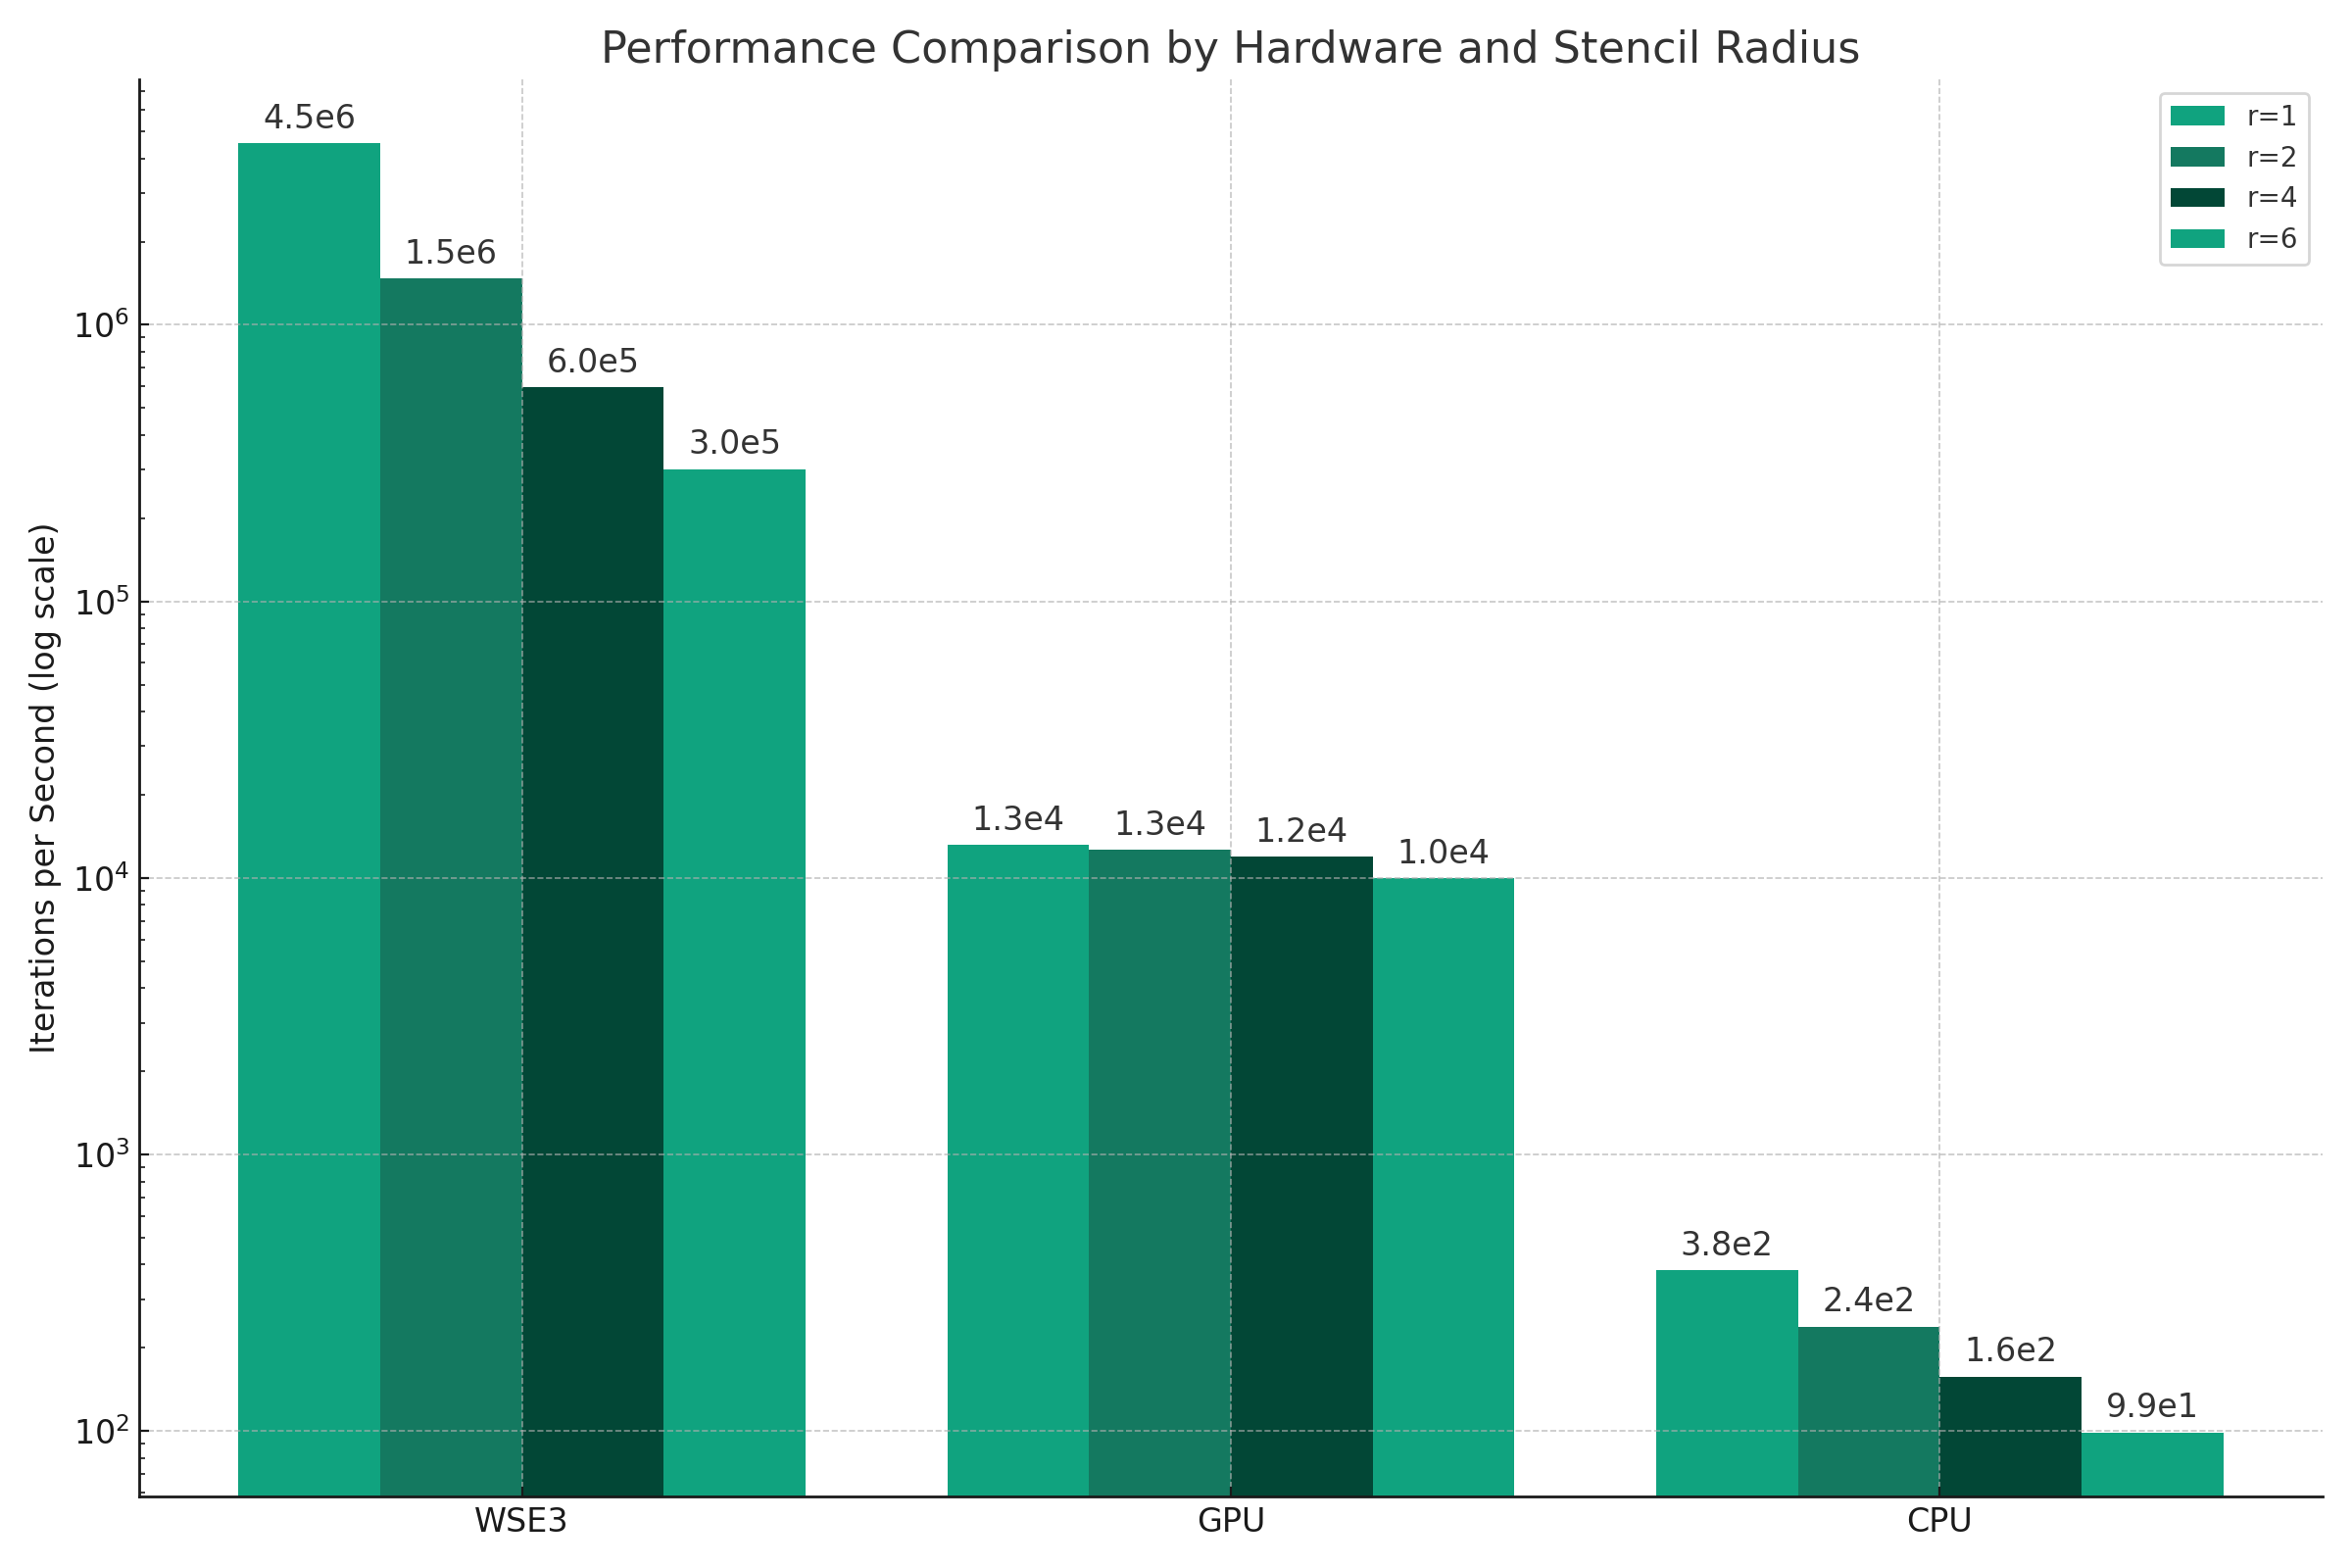
\includegraphics[width=0.5\linewidth]{cpu_gpu_cerebras_comparison.png}
%     \caption{Performance comparison across architectures for a $10^3 \times 10^4$ grid. The Cerebras \ac{wse}-3 implementation significantly outperforms the \ac{gpu} (NVIDIA H100) and \ac{cpu} (AMD EPYC 9554) across all radii. While the \ac{gpu} performance is largely insensitive to the stencil radius, indicating a memory-bound workload, the \ac{cpu} and \ac{wse}-3 performance degrades as the computational cost increases.}
%     \label{fig:cpu_gpu_cerebras_comparison}
% \end{figure}

% While the times for the \ac{gpu} and \ac{cpu} for this experiment where directly measured, we used the cycle count per iteration from the simulator for a significantly smaller grid size and a small iteration count, assumed perfect scaling to the full \ac{wse} dimensions as suggested from \autoref{sec:pe_overhead}, a constant cycle count per iteration and the clock speed of the \ac{wse} to calculate the time per iteration.

% The speedup for radius 1 from \ac{cpu} to \ac{gpu} is about 40x. From \ac{gpu} to \ac{wse}-3 we observe an even larger speedup of about 358x. As the problem is compute bound on cerebras while it is memory bound on \ac{gpu}, the speedup for radius 4 from \ac{gpu} to \ac{wse}-3 is significantly smaller at about 53x


To evaluate the performance advantage of the specialized non-tiled algorithm, we compare it directly with highly optimized implementations on traditional \ac{hpc} architectures using grid sizes that match the \ac{wse} dimensions. This comparison uses the actual \ac{wse} grid dimensions as the problem size, which represents the maximum grid size achievable with the non-tiled algorithm.

For \ac{wse}-2 with dimensions \numproduct{750 x 994} and \ac{wse}-3 with dimensions \numproduct{762 x 1176}, we measured the performance of the same radius-1 stencil on all three architectures.

\begin{figure}[h]
    \centering
    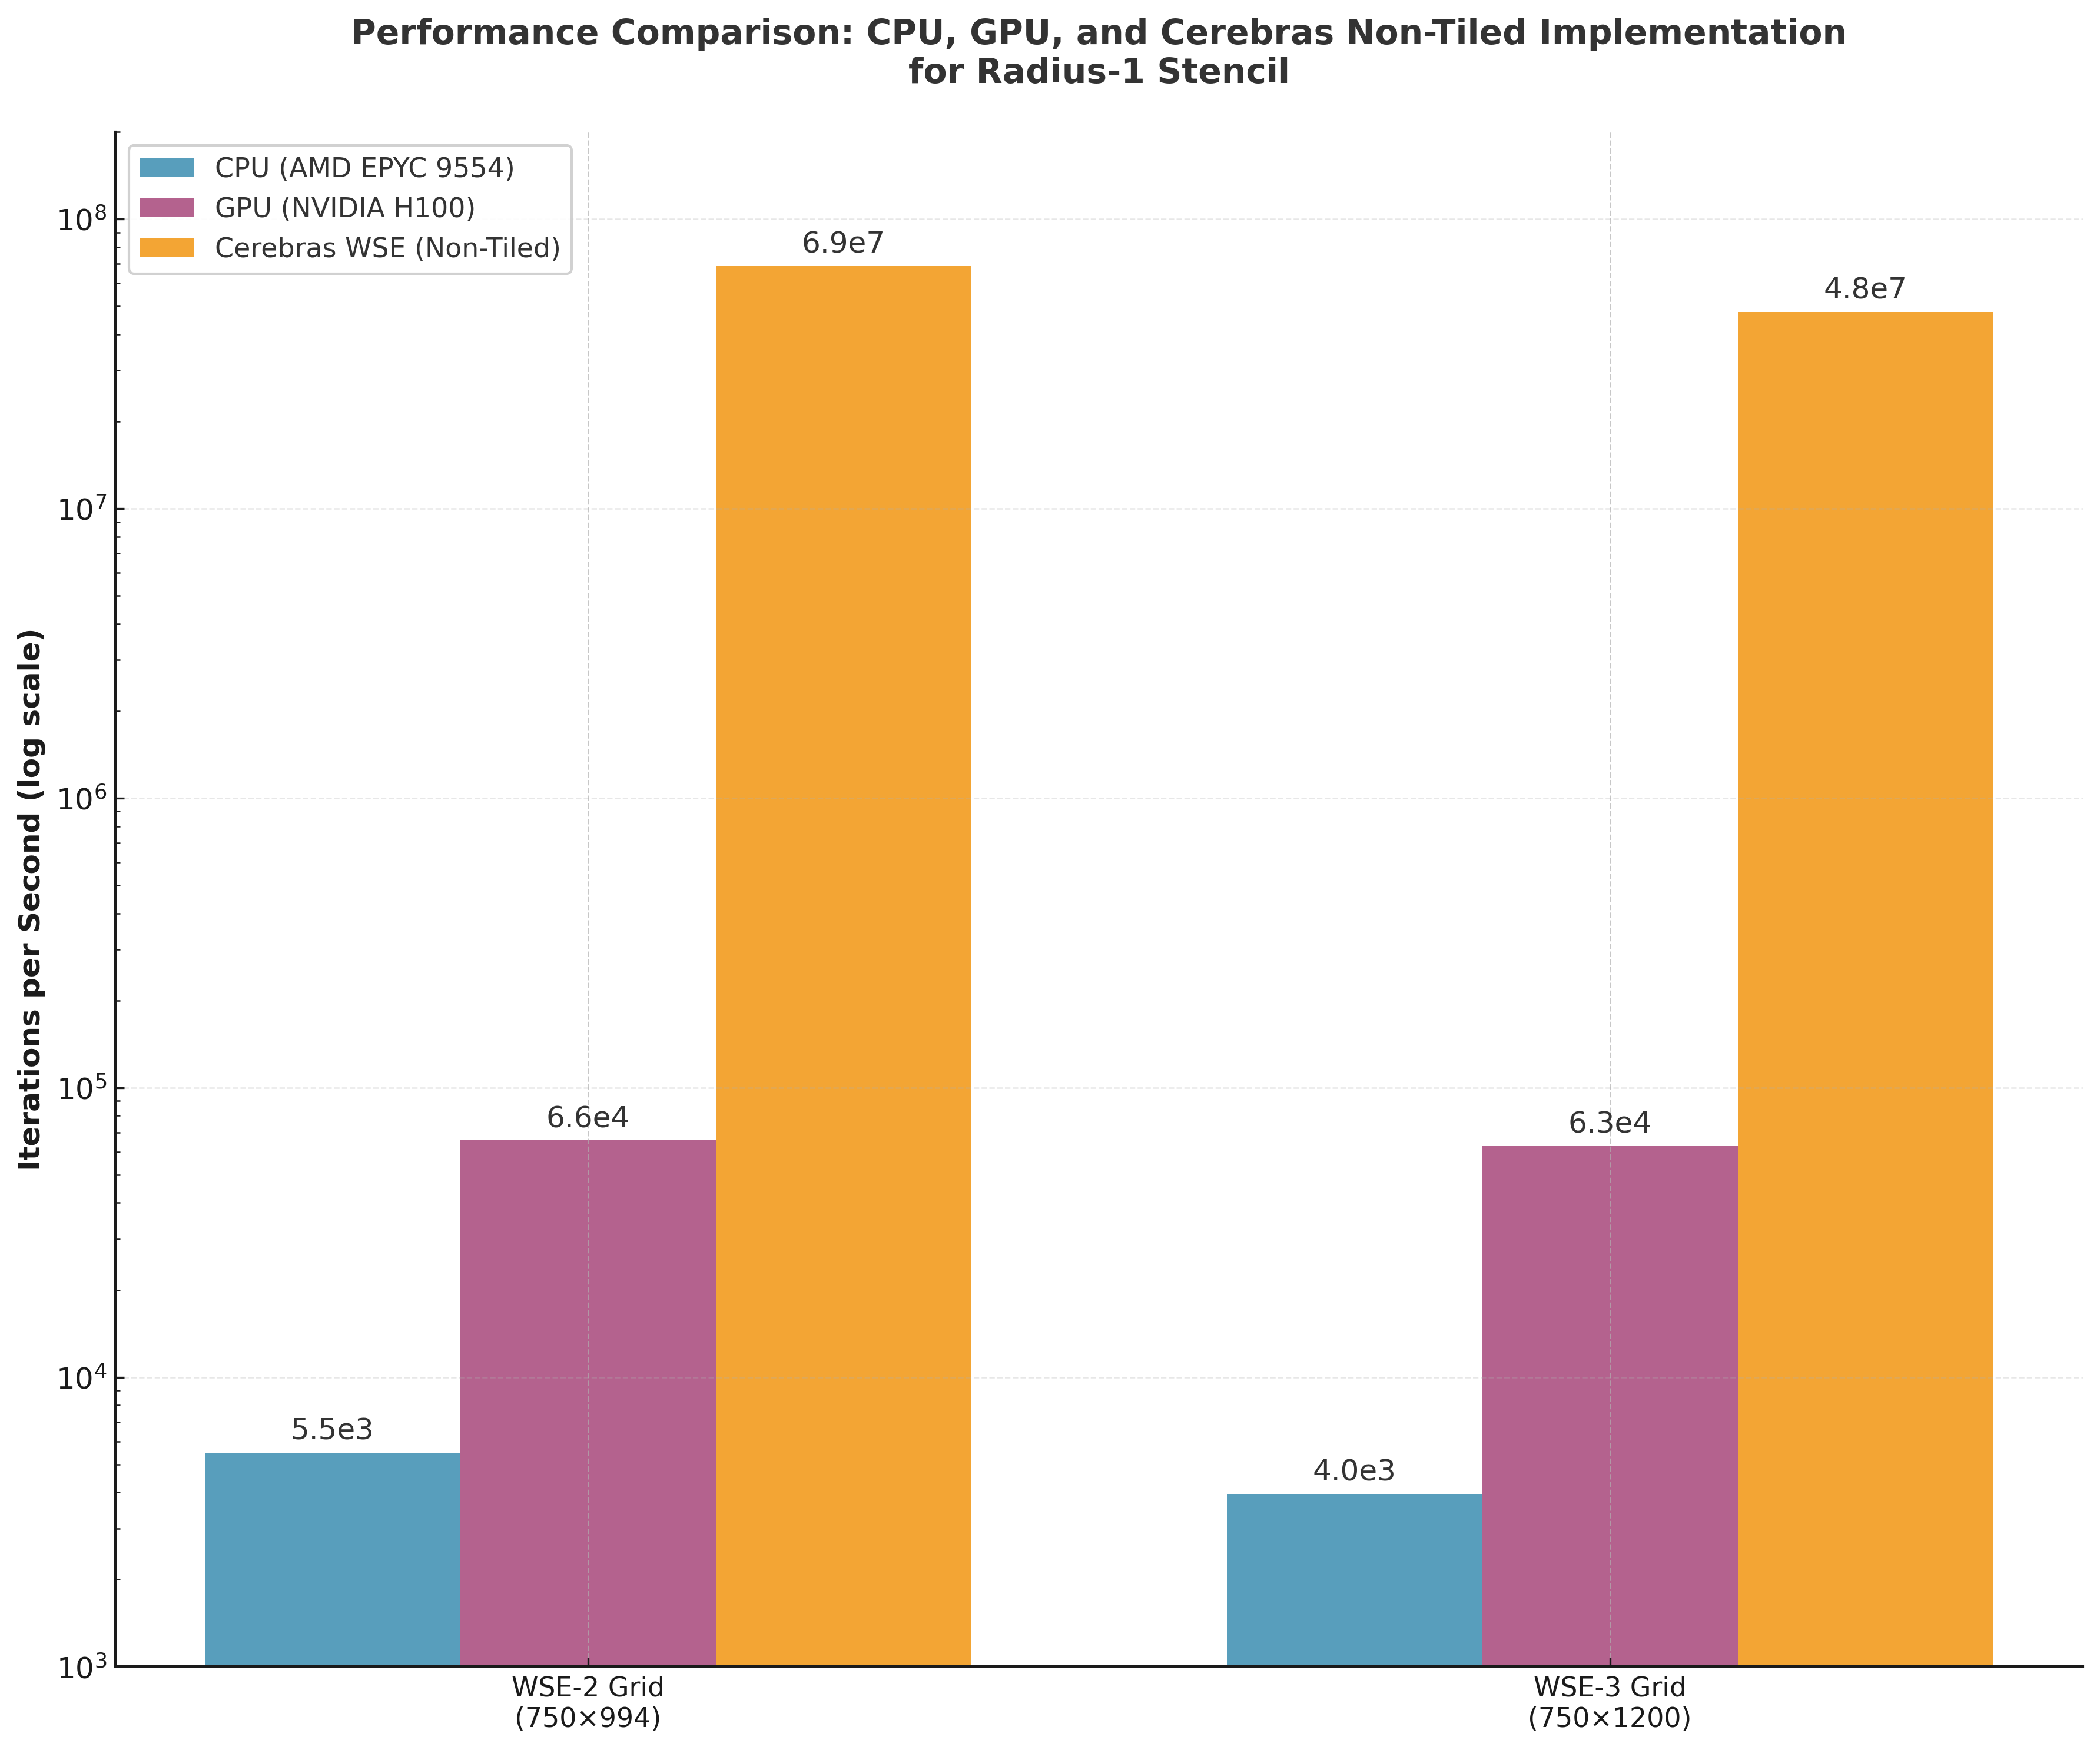
\includegraphics[width=0.7\linewidth]{cpu_gpu_cerebras_non_tiled_comparison.png}
    \caption{Performance comparison of the non-tiled Cerebras implementation against traditional \ac{hpc} architectures for radius-1 stencils. Results show iterations per second for grid sizes matching the \ac{wse} dimensions. The non-tiled algorithm achieves speedups of over 1000x compared to \ac{gpu} and over 12,000x compared to \ac{cpu}.}
    \label{fig:cpu_gpu_cerebras_non_tiled_comparison}
\end{figure}

The results demonstrate the exceptional performance of the non-tiled algorithm. For the \ac{wse}-2 grid size (\numproduct{750 x 994}), the Cerebras implementation achieves \num{68750000} iterations per second, compared to \num{65707} for the \ac{gpu}. This represents a speedup of 1046x.
For the \ac{wse}-3 grid size (\numproduct{762 x 1176}), the Cerebras implementation achieves \num{47826087} iterations per second, compared to \num{62743} for the \ac{gpu} with a speedup of 762x.

The performance advantage stems from the direct mapping of grid elements to \acp{pe}, enabling defacto in-memory computation with a memory that is significantly faster than the \ac{gpu} memory. While this approach is limited to grid sizes not exceeding the \ac{wse} dimensions, it provides unparalleled performance for problems that fit within these constraints.

\section{Percentage of peak performance}
Using the cycle counts per iteration from the simulator, we calculated the percentage of the \ac{wse}-2 and \ac{wse}-3 peak fp32 performance for different tile sizes and radii.
As described in \autoref{sec:implementation}, the non-tiled implementation and the r1-optimized implementation use \num{6} flops per grid element and iteration while the general tiled implementation uses \num{9} flops per grid element and iteration. From the respectively used tiled sizes in the different experiments, we first calculate the total number of flops per iteration and \ac{pe} and then divide by the measured cycle count per iteration to get an average flops per cycle and \ac{pe}. We find that the maximum number of fp32 operations per cycle and \ac{pe} can be obtained with \texttt{@fadds} instructions, which support a simd width of 2 in \ac{wse}-2 and 4 in \ac{wse}-3, while \texttt{@fmacs} is not supported in simd mode. Using the calculated average flops per cycle and \ac{pe} and the maximum flops per cycle and \ac{pe}, we calculate the percentage of the peak performance \autoref{fig:percent_pflops}.

\begin{figure}[h]
    \centering
    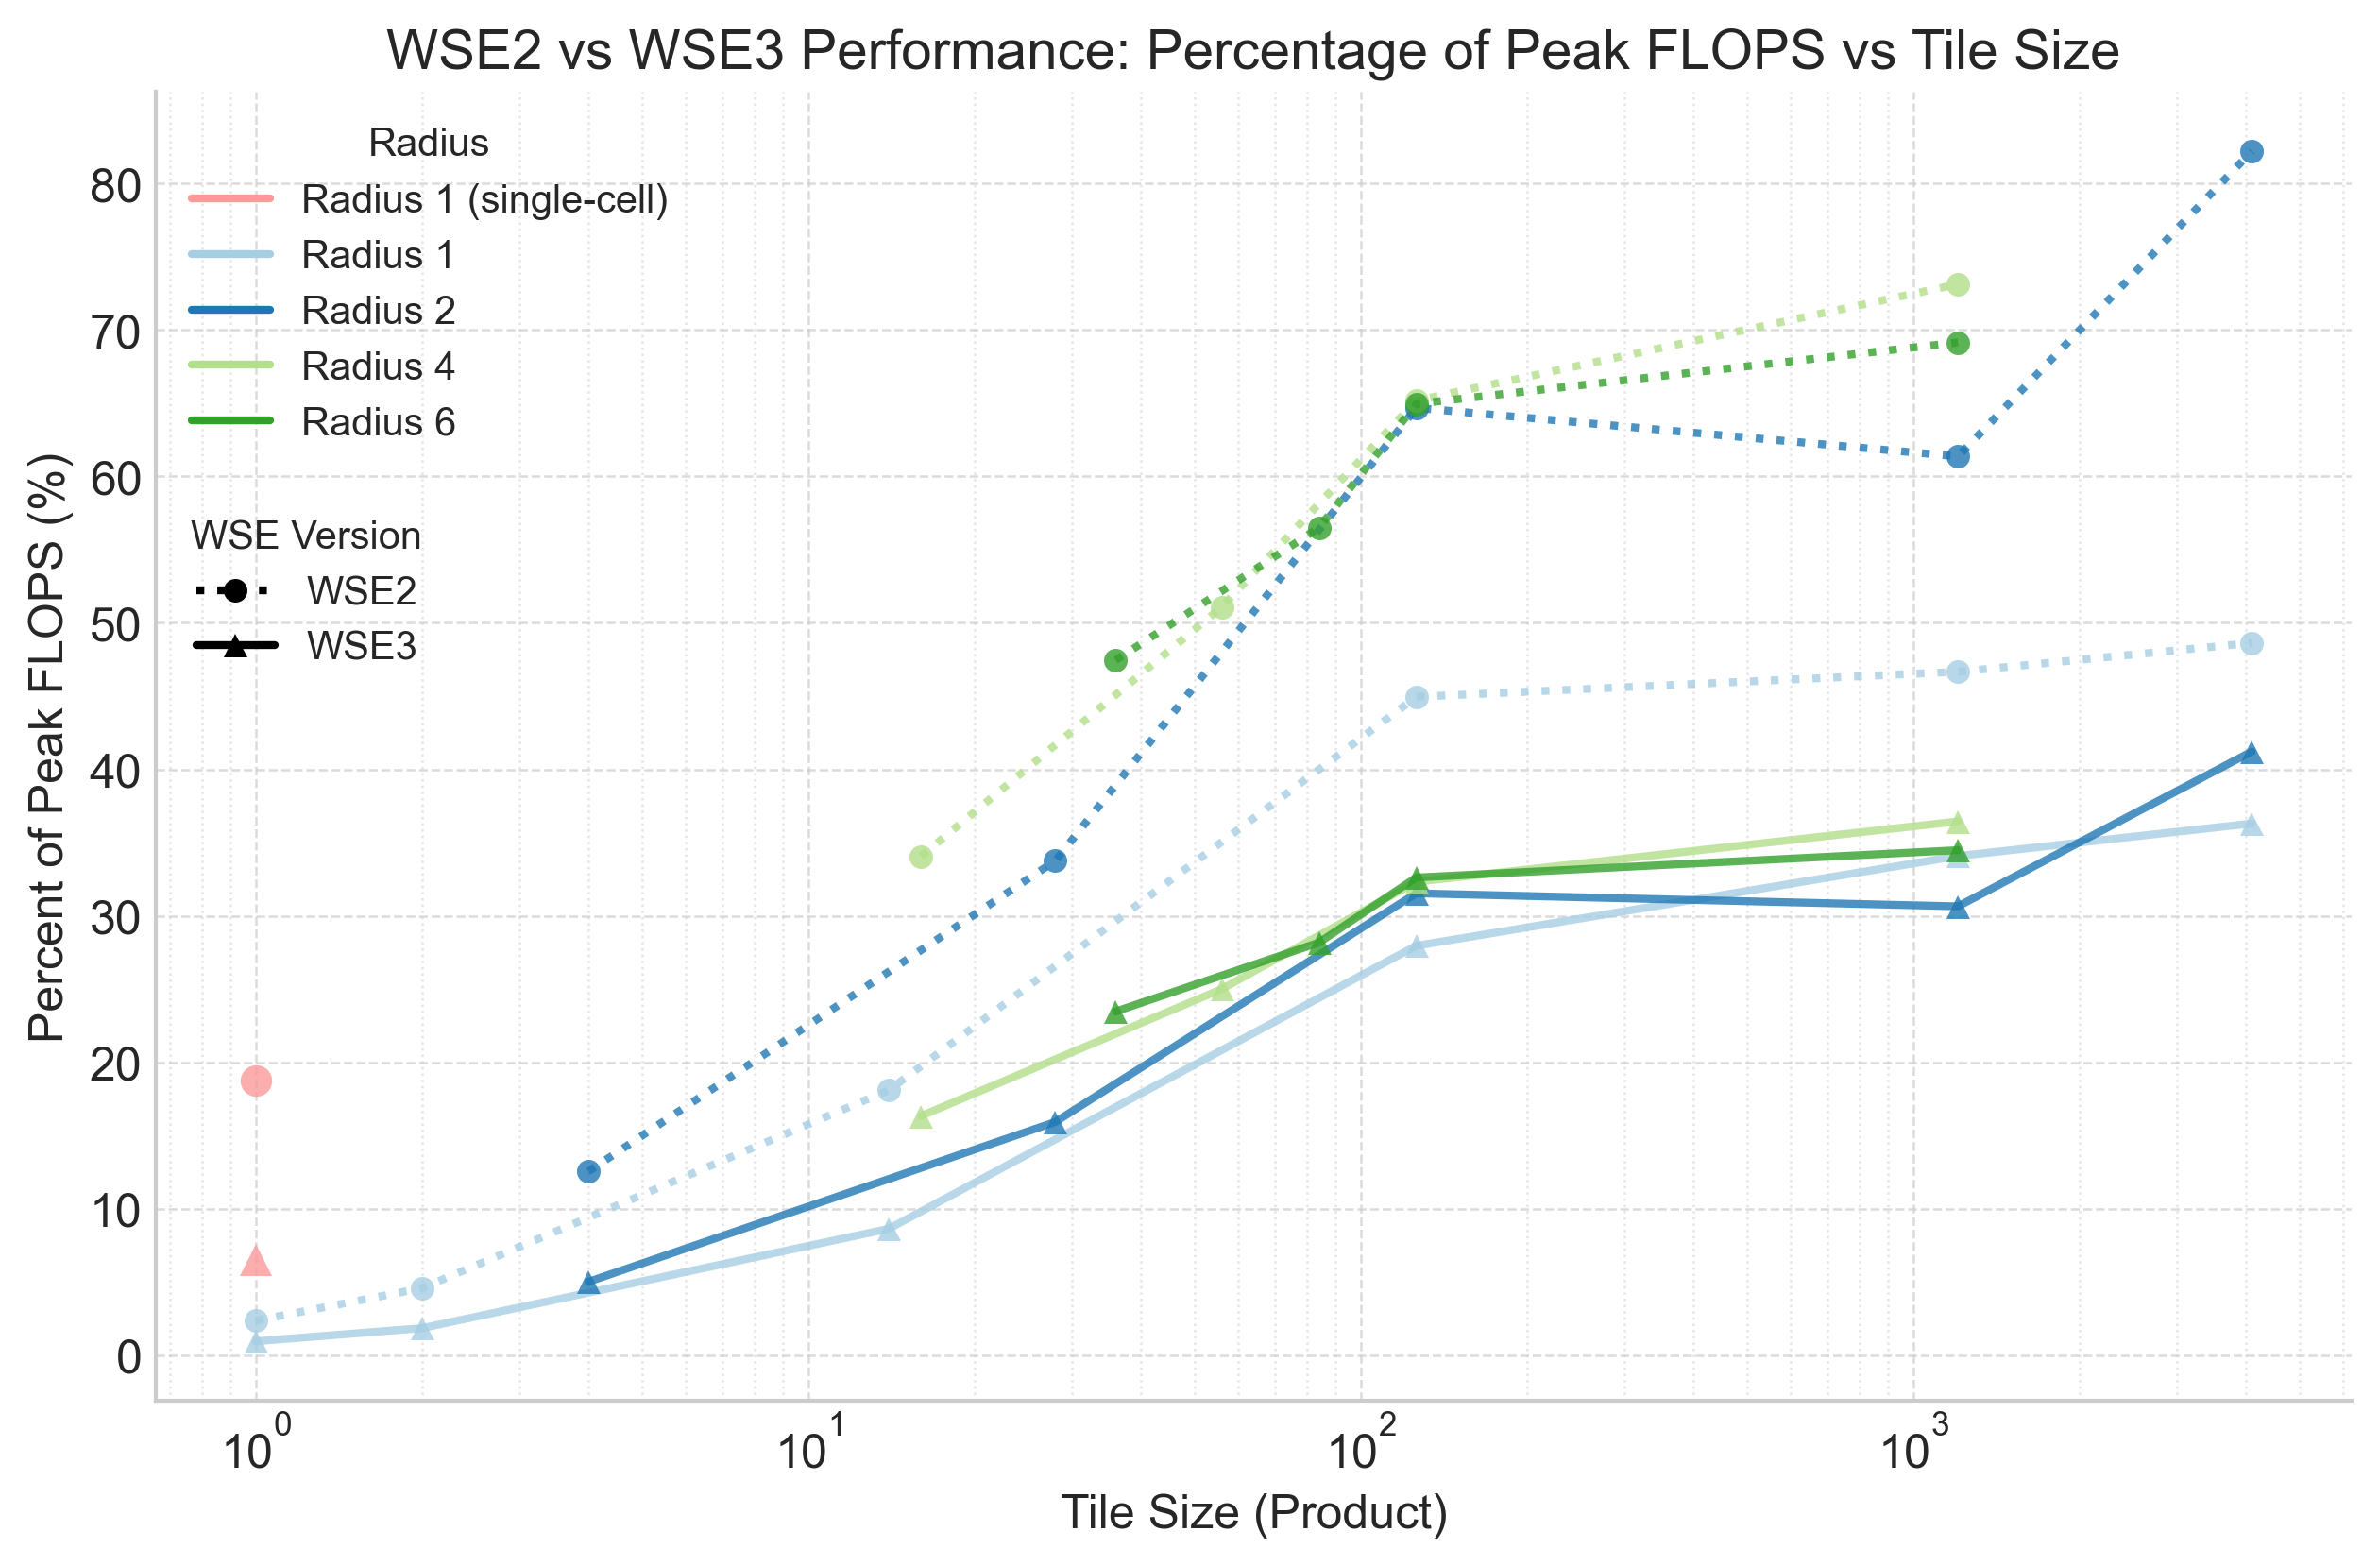
\includegraphics[width=0.7\linewidth]{percent_pflops.png}
    \caption{Percentage of peak performance for different tile sizes and radii for \ac{wse}-2 and \ac{wse}-3.}
    \label{fig:percent_pflops}
\end{figure}

For radius 1, and the maximum tile size of \numproduct{64 x 64} we reach \num{48}\% of the peak performance for \ac{wse}-2 and \num{36}\% for \ac{wse}-3.
While these numbers are per \ac{pe}, they also hold for the entire system, if the problem size is large enough to use the whole \ac{wse} dimensions.
In general, the archived percentage of peak performance mostly increases with the tile size and decreases with the radius.

In the optimal configuraion, our implementation reaches a sustained performance of 800 (797,6) TFLOP/s for \ac{wse}-2 and 1430 (1431,3) TFLOP/s for \ac{wse}-3.

\section{What contributes to the cycle count?}
We analyze the the instruction traces the simulator can record for what contributes to the the measured cycle counts.
We find that the effective simd width for some instructions in our implementation is lower than the theoretical maximum.
For \texttt{@fadds} it is 1.25 on wse-2 and 1.5 on wse-3.
The \texttt{@fmuls} instruction only have a simd width of 1 and we find that we measure exactly one cycle per instruction.

Here is a table that lists the different number of cycles per program segment. 
% \chapter{Discussion}
- why not full simd width?
- answer research questions from introduction
- why is wse3 slower than wse2? 
\chapter{Future Work}
\begin{itemize}
    \item 
    \item More optimization: use border \acp{pe} in a smarter way, use explicit \ac{dsr} assignment,try to overlap communication and computation in the general algorithm
    \item try achieving full simd width (lower precision data types??)
    \item JOR, Gauss-Seidel / Red-Black implentation and SOR method or multigrid methods
    \item automatic convergence detection
\end{itemize} 


variable coefficients accross the grid. while not implemented in this work, should be easy and without performance overhead.

asymetric coefficients. Not that hard to extend to. should have no performance overhead for tiled implementation except r1 optimized implementation that uses pv1+pv2+pv3+pv4=p(v1+v2+v3+v4) as optimization strategy, which is not applicable for asymetric coefficients.

non-linear stencils would invole more work to implement and potentially optimize.

extend to box shaped stencils,

% % Bibliography is handled automatically by the template 
\clearpage
%------------------------------
% REFERENCES
%------------------------------
\printbibliography[category=inbib,resetnumbers]
%------------------------------
% APPENDIX
%------------------------------
\appendix
\chapter{Appendix}
\section{Usage of \ac{ai}}
Throughout this thesis, we used generative \ac{ai} systems for various tasks.
Below is an explanation of each type of task and how we used \ac{ai} to assist us.

\subsection{Code Generation}
The core of this thesis, the kernel code in \ac{csl}, was manually written by the author. Current \ac{ai} systems are not capable of generating correct code for \ac{csl} due to its novelty and very limited number of open-source implementations. They also lack a deep understanding of the different programming paradigms enabled by the architecture of the \ac{wse}. Still, within the code editor Cursor, code completion at the level of "advanced copy and paste" was used to assist in the process. For other parts of the code, however, different \ac{ai} systems were used heavily to completely implement or help with implementing tasks, including setting up, running, and gathering the results for experiments and the implementation of the stencil in Devito. Most plots were generated with Matplotlib, with code mostly written by \ac{ai}.

\subsection{Systematic Research}
Deep-research \ac{ai} systems were used to help with systematic research. This included the search for relevant literature and determining the exact contributions of specific papers. Furthermore, they were used to gain a broad understanding of stencil computations, their applications, and how stencils can be categorized.

\subsection{Writing}
To improve the quality of the writing, \ac{ai} systems were used to proofread the text, double-check calculations, correct grammar and spelling mistakes, gather high-level feedback about the correctness and understandability of the text, and improve the structure of the text and provide suggestions for improvements. \ac{ai} was also used to translate the abstract.

\subsection{List of \ac{ai} Systems Used}
The following is a list of the \ac{ai} systems used, the organization they were developed by, and their purpose:

\begin{table}[H]
    \centering
    \begin{tabular}{>{\raggedright\arraybackslash}p{4cm}>{\raggedright\arraybackslash}p{2cm}>{\raggedright\arraybackslash}p{2cm}>{\raggedright\arraybackslash}p{4cm}}
        \toprule
        Product name & Manufacturer & Version & Purpose \\
        \midrule
        Cursor & Anysphere & 1.0.0 & Code completion \\
        Gemini & Google & 2.5 Pro & Writing, systematic research, code generation \\
        Deep Research powered by Gemini 2.5 Pro & Google & - & Systematic research \\
        Claude & Anthropic &  3.7 Sonnet & Code generation \\
        GPT & OpenAI & 4.1 & Code generation \\
        o3 & OpenAI & - & Code generation, Writing (especially for checking math) \\
        Deep Research powered by o3-mini & OpenAI & - & Systematic research \\
    \end{tabular}
\end{table}	% include appendices
\clearpage
%------------------------------
% INDEX
%------------------------------
% \printindex
%------------------------------
% END DOCUMENT
%------------------------------
\end{document}